% --------------------------------------------------------------------
\section{Energy Conservation (First Law) for Open Systems}
% --------------------------------------------------------------------
In this course we consider three types of {\bf open systems} - steam power plants, refrigeration systems, and aircraft jet engines. These are complex systems, but we will break them down into components, then separately analyze each component. Figure \ref{fig:ch4_controlVolume} shows a representative component with mass flow, shaft work, and heat transfer.

\begin{figure}[H]
\centering
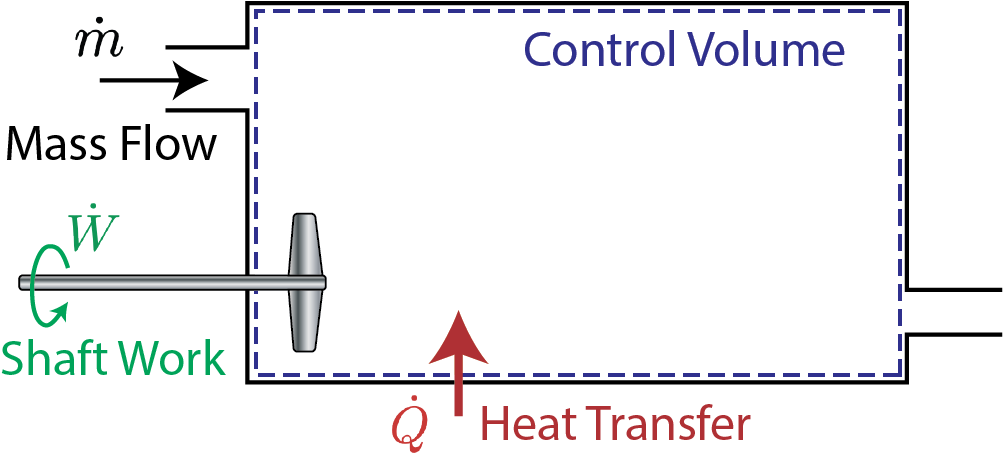
\includegraphics[width=0.75\textwidth]{ControlVolume}
\caption{Diagram of a control volume (open system).}
\label{fig:ch4_controlVolume}
\end{figure}

For every component we analyze in this class, we will assume that there will be no change over time inside the component.  This is a very reasonable assumption as long as the component has be running for a while without any changes to its conditions.  This is commonly known as the {\bf steady-state} assumption.

For open systems, the consistent mass flow rate means that our components operate continuously, rather than through cycles.  While we calculated the amount of energy in one cycle of operation for closed systems, we will calculate the amount of energy in one second of operation for open systems.  Thus, it is typically more convenient to use power [kW] rather than energy [kJ].  The mass specific energy [kJ/kg] will still be useful in our analyses.

% --------------------------------------------------------------------
\subsection{Mass Flow}

%Consider a differential mass $dm$ flowing through an inlet or outlet port of a control volume, having an area $A$, volume $dV$, length $dx$, and an average steady velocity $\vec{V}$, as follows.

%\begin{figure}[H]
%\centering
%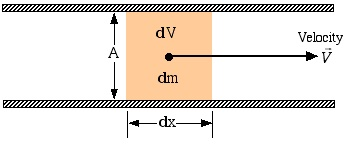
\includegraphics[width=0.75\textwidth]{massFlow}
%\caption{The movement of a differential mass element through a control volume.}
%\label{fig:ch3_massFlow}
%\end{figure}

Looking again at Figure \ref{fig:ch4_controlVolume}, let's start by saying the change of mass inside the control volume, $m_{cv}$ is equal to the mass entering, $\dot{m}_{in}$, minus the mass leaving, $\dot{m}_{out}$.  The sums in Equation \ref{eq:ch4_massAccounting} are there to indicate that we may have multiple inlets and outlets in our problem.
\begin{equation} \label{eq:ch4_massAccounting}
  \frac{\partial m_{cv}}{\partial t} = \sum \dot{m}_{in} - \sum \dot{m}_{out}
\end{equation}

Assuming steady-state flow allows us to remove $\frac{\partial m_{cv}}{\partial t}$, as there should not be any change with respect to time:
\begin{equation} \label{eq:ch4_mdot}
  \sum \dot{m}_{in} = \sum \dot{m}_{out} = \dot{m}
\end{equation}



%Even if we assume steady-state flow (meaning no change in time), we can still have a {\bf mass flow rate}, represented by $\dot{m}$.  We can rewrite $\dot{m}$ by integrating across the boundary of the control volume:
%\begin{align*}
%  \dot{m}_{in} &= \int_{inlet} \rho \vec{V} dA \\
%  \dot{m}_{out} &= \int_{outlet} \rho \vec{V} dA
%\end{align*}

%Assuming that the density and velocity are constant across the inlet/outlet allows us to build a much simpler form.
%\begin{align*}
%  \dot{m}_{in} &= \rho_{in}\vec{V}_{in}A_{in} \\
%  \dot{m}_{out} &= \rho_{out}\vec{V}_{out}A_{out}
%\end{align*}

For a steady-state control volume with a single exit and outlet, we can simplify to the following:
\begin{equation*}
  \dot{m}_{in} = \dot{m}_{out} = \dot{m}
\end{equation*}

In other words, the mass flow must be a constant value through each component for a steady-state problem.

%We can create several alternate forms for the mass flow rate:
%\begin{equation}\label{eq:ch4_massFlow}
%  \dot{m} = \rho A \vec{V} = \frac{A\vec{V}}{v} = \frac{Q}{v}
%\end{equation}

%$Q$ is known as the {\bf volumetric flow rate}.

% --------------------------------------------------------------------
\subsection{Flow Work}

The fluid mass flows through the inlet and exit ports of the control volume.  As it flows in, it performs pressure work on the fluid inside the control volume.  This {\bf flow work} is equivalent to the amount of work it would take to move a piston at the pressure of the incoming fluid.

\begin{figure}[H]
\centering
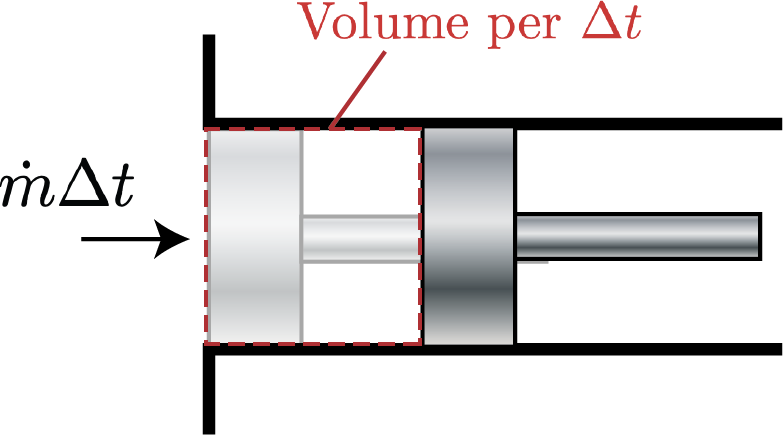
\includegraphics[width=0.6\textwidth]{FlowWork}
\caption{Fluid entering a control volume performs work just as if it were moving a piston.}
\label{fig:ch3_flowWork}
\end{figure}

Let us calculate the amount of work done by the flow coming in over a time $\Delta t$.
\begin{equation} \label{eq:ch4_flowWork}
  W_{flow} = \int F\,dx = \int_0^V p\, dV = pV = mpv
\end{equation}

In other words, the amount of work done in $\Delta t$ is equal to the pressure of the incoming flow times the amount of volume of fluid coming in over the same time period.

Considering the time that the operation takes, we rearrange Equation \ref{eq:ch4_flowWork} as follows:
\begin{equation*}
  \frac{W_{flow}}{\Delta t} = \frac{mpv}{\Delta t} \qquad \rightarrow \qquad
  \dot{W}_{flow} = \dot{m}pv
\end{equation*}

The dotted values simply represent the quantity of work or mass {\bf per unit time}.  Thus, we can say that $m = \dot{m}\Delta t$.

We can define specific values in a similar manner to closed systems by using $\dot{m}$ instead of $m$:
\begin{equation} \label{eq:ch4_specificFlowWork}
  w_{flow} = \frac{\dot{W}_{flow}}{\dot{m}} = pv
\end{equation}

This result will be useful as we develop the complete energy equation in the next section.

% --------------------------------------------------------------------
\subsection{Conservation of Energy for an Open System}
Let's look again at a sample control volume, but this time we will consider energy flow instead of mass flow.

\begin{figure}[H]
\centering
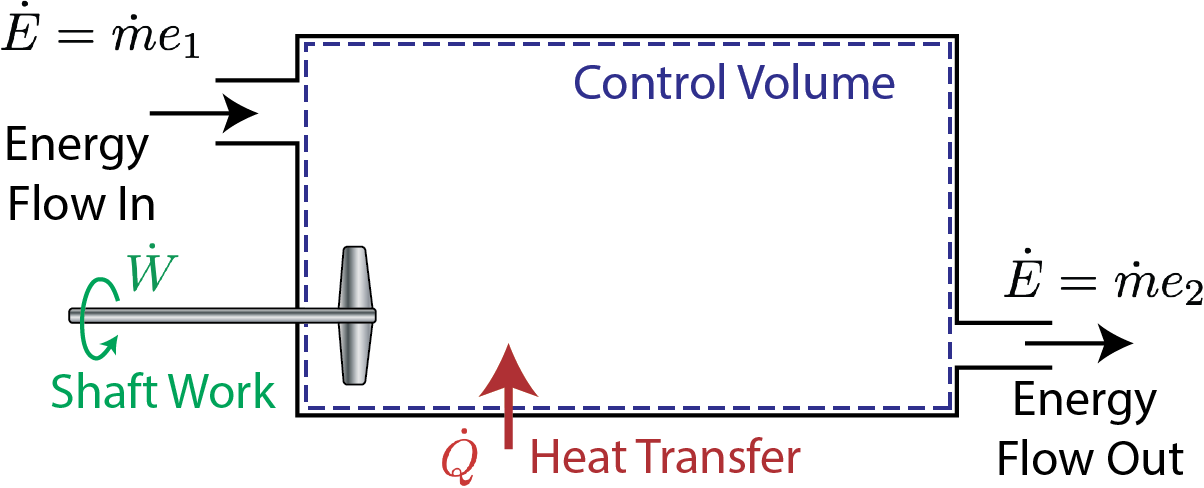
\includegraphics[width=0.6\textwidth]{ControlVolumeEnergy}
\caption{Diagram showing all sources of energy affecting an open system.}
\label{fig:ch4_CVenergyConservation}
\end{figure}

Figure \ref{fig:ch4_CVenergyConservation} shows that energy enters the control volume through mass flow at 1 ($\dot{m} e_1$) and through heat transfer ($\dot{Q}$) and work ($\dot{W}$).  Likewise, energy leaves the control volume through mass flow at 2 ($\dot{m} e_2$). As in closed systems, work is defined such that work performed on the system is negative.

\begin{equation*}
  \dot{m} e_1 + \dot{Q} - \dot{W} = \dot{m} e_2
\end{equation*}

At this point, we should talk about the energy, $e$.  There are many different types of energy, and in the broadest sense, $e$ incorporates all of them.  We've discussed potential, kinetic, and internal energy back in Chapter 1.  We could also include chemical energy (combustion, etc.), nuclear energy (for nuclear reactors), or other more exotic forms.  For the sake of this discussion, we will limit ourselves to the three types discussed in Chapter 1.

\begin{equation} \label{eq:energyDefinition}
  e = u + \frac{1}{2}\vec{V}^2 + gz
\end{equation}

The $\dot{W}$ term will encompass three types of work.  First, we will incorporate the flow work from Equation \ref{eq:ch4_flowWork}.  Then, we will split our shaft work into work done to the system by pumps and compressors ($\dot{W}_{pumps}$) and work extracted from the system by turbines ($\dot{W}_{turbines}$).

\begin{equation} \label{eq:flowWork}
  \dot{W} = \dot{m}(p_2 v_2 - p_1 v_1) - \dot{W}_{pumps} + \dot{W}_{turbines}
\end{equation}

Our energy equation now has the following form:
\begin{equation*}
  \dot{m}\left(u_1 + \frac{1}{2}\vec{V_1}^2 + gz_1\right) + \dot{Q} - \left(\dot{m}(p_2 v_2 - p_1 v_1) -\dot{W}_{pumps} + \dot{W}_{turbines}\right)= \dot{m}\left(u_2 + \frac{1}{2}\vec{V_2}^2 + gz_2\right)
\end{equation*}

We can distribute the flow work to group it with the other forms of energy, and move the $\dot{W}$ terms to the right hand side:
\begin{equation*}
  \dot{m}\left(u_1 + p_1v_1 + \frac{1}{2}\vec{V_1}^2 + gz_1\right) + \dot{Q} = \dot{m}\left(u_2 + p_2v_2 + \frac{1}{2}\vec{V_2}^2 + gz_2\right) -\dot{W}_{pumps} + \dot{W}_{turbines}
\end{equation*}

Using the definition of enthalpy from Section \ref{sec:ch3_enthalpy}, we recognize that $u+pv = h$.
\begin{equation} \label{eq:controlVolumeEnergyEquation}
  \dot{m}\left(h_1 + \frac{1}{2}\vec{V_1}^2 + gz_1\right) + \dot{Q} = \dot{m}\left(h_2 + \frac{1}{2}\vec{V_2}^2 + gz_2\right) -\dot{W}_{pumps} + \dot{W}_{turbines}
\end{equation}

For many problems, we neglect the effects of kinetic and potential energy.  In those situations, we can further simplify:
\begin{equation*} 
  \dot{m}h_1 + \dot{Q} = \dot{m}h_2 -\dot{W}_{pumps} + \dot{W}_{turbines}
\end{equation*}

If we define $\Delta h = h_2 - h_1$, we can get an equation very similar to Equation \ref{eq:1stLawClosed}.
\begin{equation}
  \label{eq:controlVolumeEnergyNoKEPE}
  \dot{m} \Delta h = \dot{Q} + \dot{W}_{pumps} - \dot{W}_{turbines}
\end{equation}

Finally, we can get the specific form of the equation by dividing through by $\dot{m}$.
\begin{equation}\label{eq:ch4_firstLawOpenSystems}
  \Delta h = q + w_{pumps} - w_{turbines}
\end{equation}

Notice that enthalpy $h$ is fundamental to the energy equation for open systems.

% --------------------------------------------------------------------
\section{The $p$-$h$ (Pressure-Enthalpy) Diagram}

  When dealing with closed systems we found that sketching $T$-$v$ or $p$-$v$ diagrams was a significant aid in describing and understanding the various processes. In steady flow systems we find that the pressure-enthalpy ($p$-$h$) diagrams serve a similar purpose, and we will use them extensively. In this course we consider two pure fluids - water and refrigerant R134a, and we have provided $p$-$h$ diagrams for each in Appendices \ref{app:phsteam} and \ref{app:phr134a}. We will illustrate their use in the following examples. The $p$-$h$ diagram for water is shown below.

  
\begin{figure}[H]
\centering
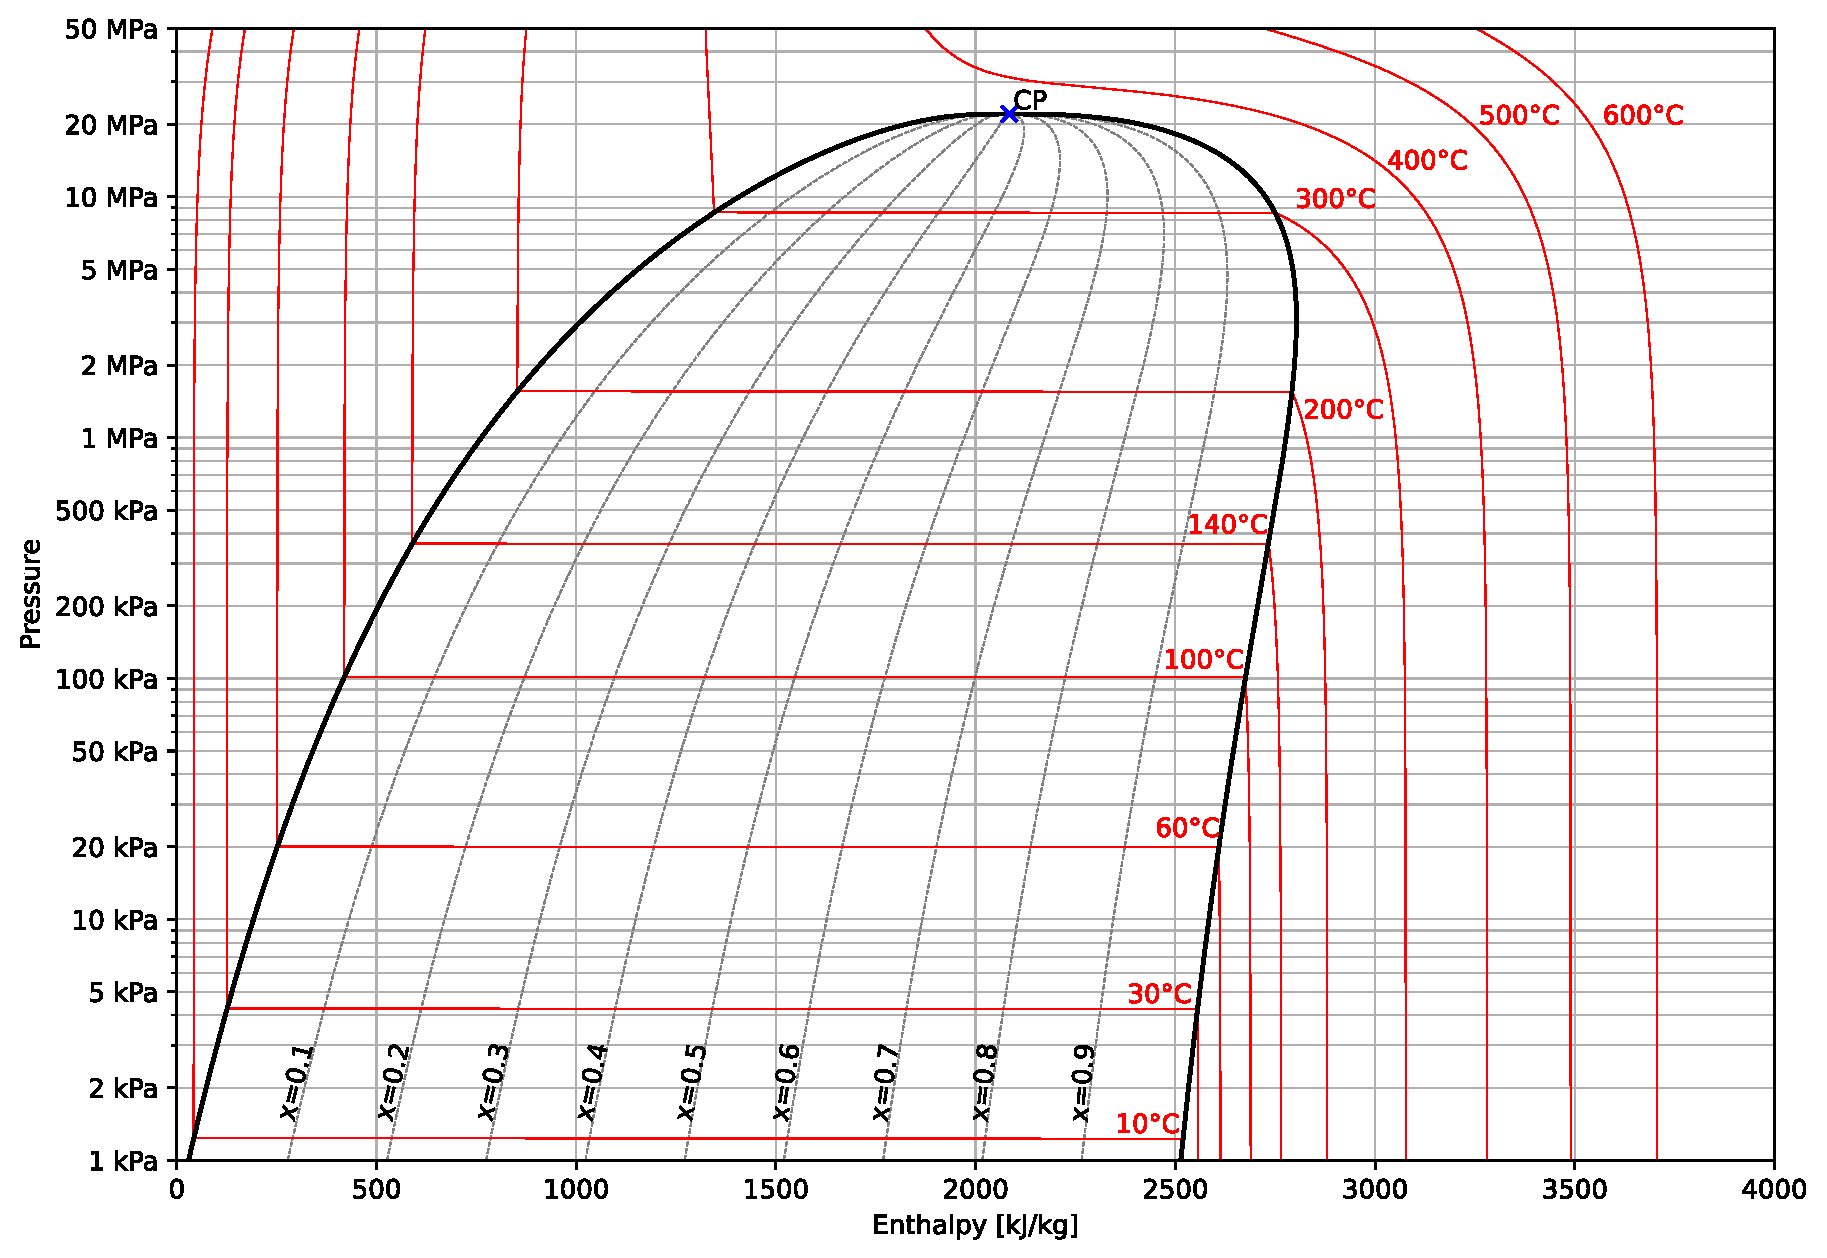
\includegraphics[width=0.9\textwidth]{p-h_water}
\caption{Pressure-enthalpy diagram for water.  Note the vertical isothermal lines at high enthalpy and low pressure (ideal gas) and for supercooled water (incompressible), as well as the horizontal isothermal lines for the saturated mixture.}
\label{fig:ch3_phWater}
\end{figure}

Importantly, in the ideal gas range, enthalpy is primarily determined by temperature ($\Delta h = c_p \Delta T$), leading to the vertical isothermal lines in that region.  The same is true in the compressed liquid, as liquids are typically incompressible.  For liquid-vapor mixtures, the enthalpy changes mostly with quality.  Finally, in the supercritical region, both temperature and pressure will have an impact on enthalpy.

% --------------------------------------------------------------------
\section{Components of Thermodynamic Systems}
% --------------------------------------------------------------------
In open systems, fluids are transferred between multiple components, each of which has a specialized purpose.  Most simply, a component will add or extract heat, perform work on the fluid as it passes through, or extract energy in the form of work from the fluid as it passes through.  This is a different paradigm from the closed systems of Chapter \ref{ch:closed_systems}, in which fluid was stuck in piston, heat was added, and work was extracted.

Cycles for open systems are created by chaining these components.  For instance, in a Rankine Power Plant (see Section \ref{sec:RankinePower}), water will move from a turbine to a condenser, then through a pump and a boiler, and finally back to the turbine.  The states are defined between the various components, and each component is described as a thermodynamic process.

The rest of this section is devoted to describing the various components.  Turbines, compressors, and pumps all deal with work. Boilers, condensers, and evaporators either add or remove heat. Finally, mixers, throttles, heat exchangers, and de-aerators all have other impacts on the fluid.

%-----------------------------------------------------------------------------
\subsection{Turbines} \label{sec:ch4_turbines}

Typically, anything that extracts work from a moving fluid (either liquid or gas) is known as a turbine.  While there are many different varieties of turbines, all of them use high pressure within the fluid to provide torque to a rotating shaft, typically by way of specially designed blades.  In the case of power plants, the rotating shaft is connected to an alternator, which turns the rotational mechanical energy into electrical energy.

\begin{figure}[H]
  \centering
  \begin{subfigure}[b]{0.55\textwidth}
    \centering
    \includegraphics[width=1.0\textwidth]{TurbineImage}
   
  \end{subfigure}
  \hfill
  \begin{subfigure}[b]{0.35\textwidth}
    \centering
    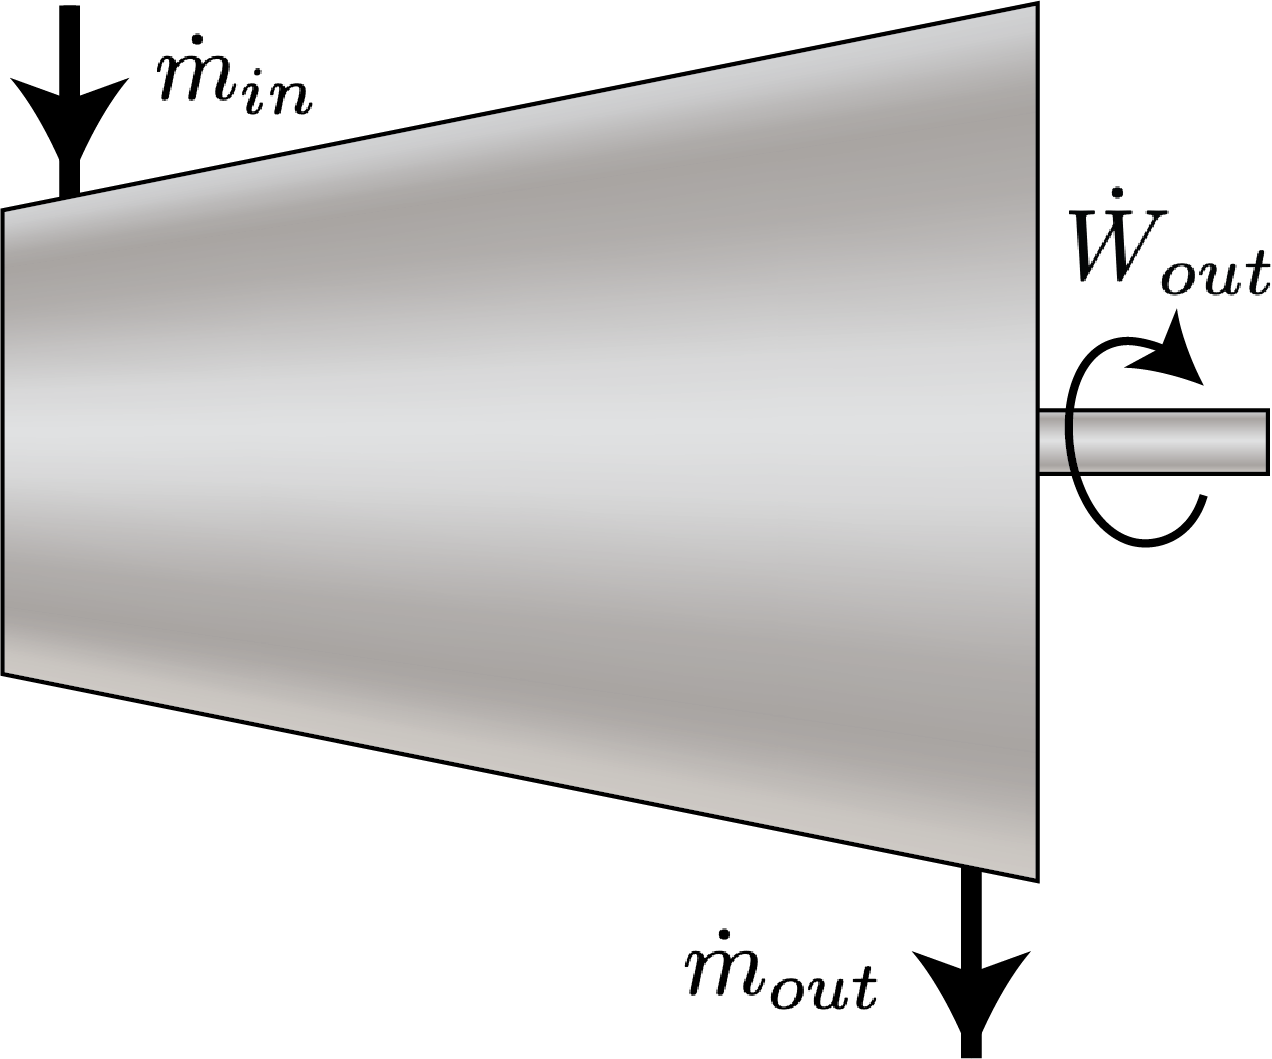
\includegraphics[width=1.0\textwidth]{TurbineDiagram}
  \end{subfigure}
   \caption{Left: From \href{https://commons.wikimedia.org/wiki/File:BalNPP_m_st2.jpg}{Wikipedia}.  A large steam turbine without its cover.  \\ Right: A typical representation of a turbine for cycle diagrams.}
\label{fig:ch4_turbineDiagram}
\end{figure}

\begin{figure}[H]
\centering
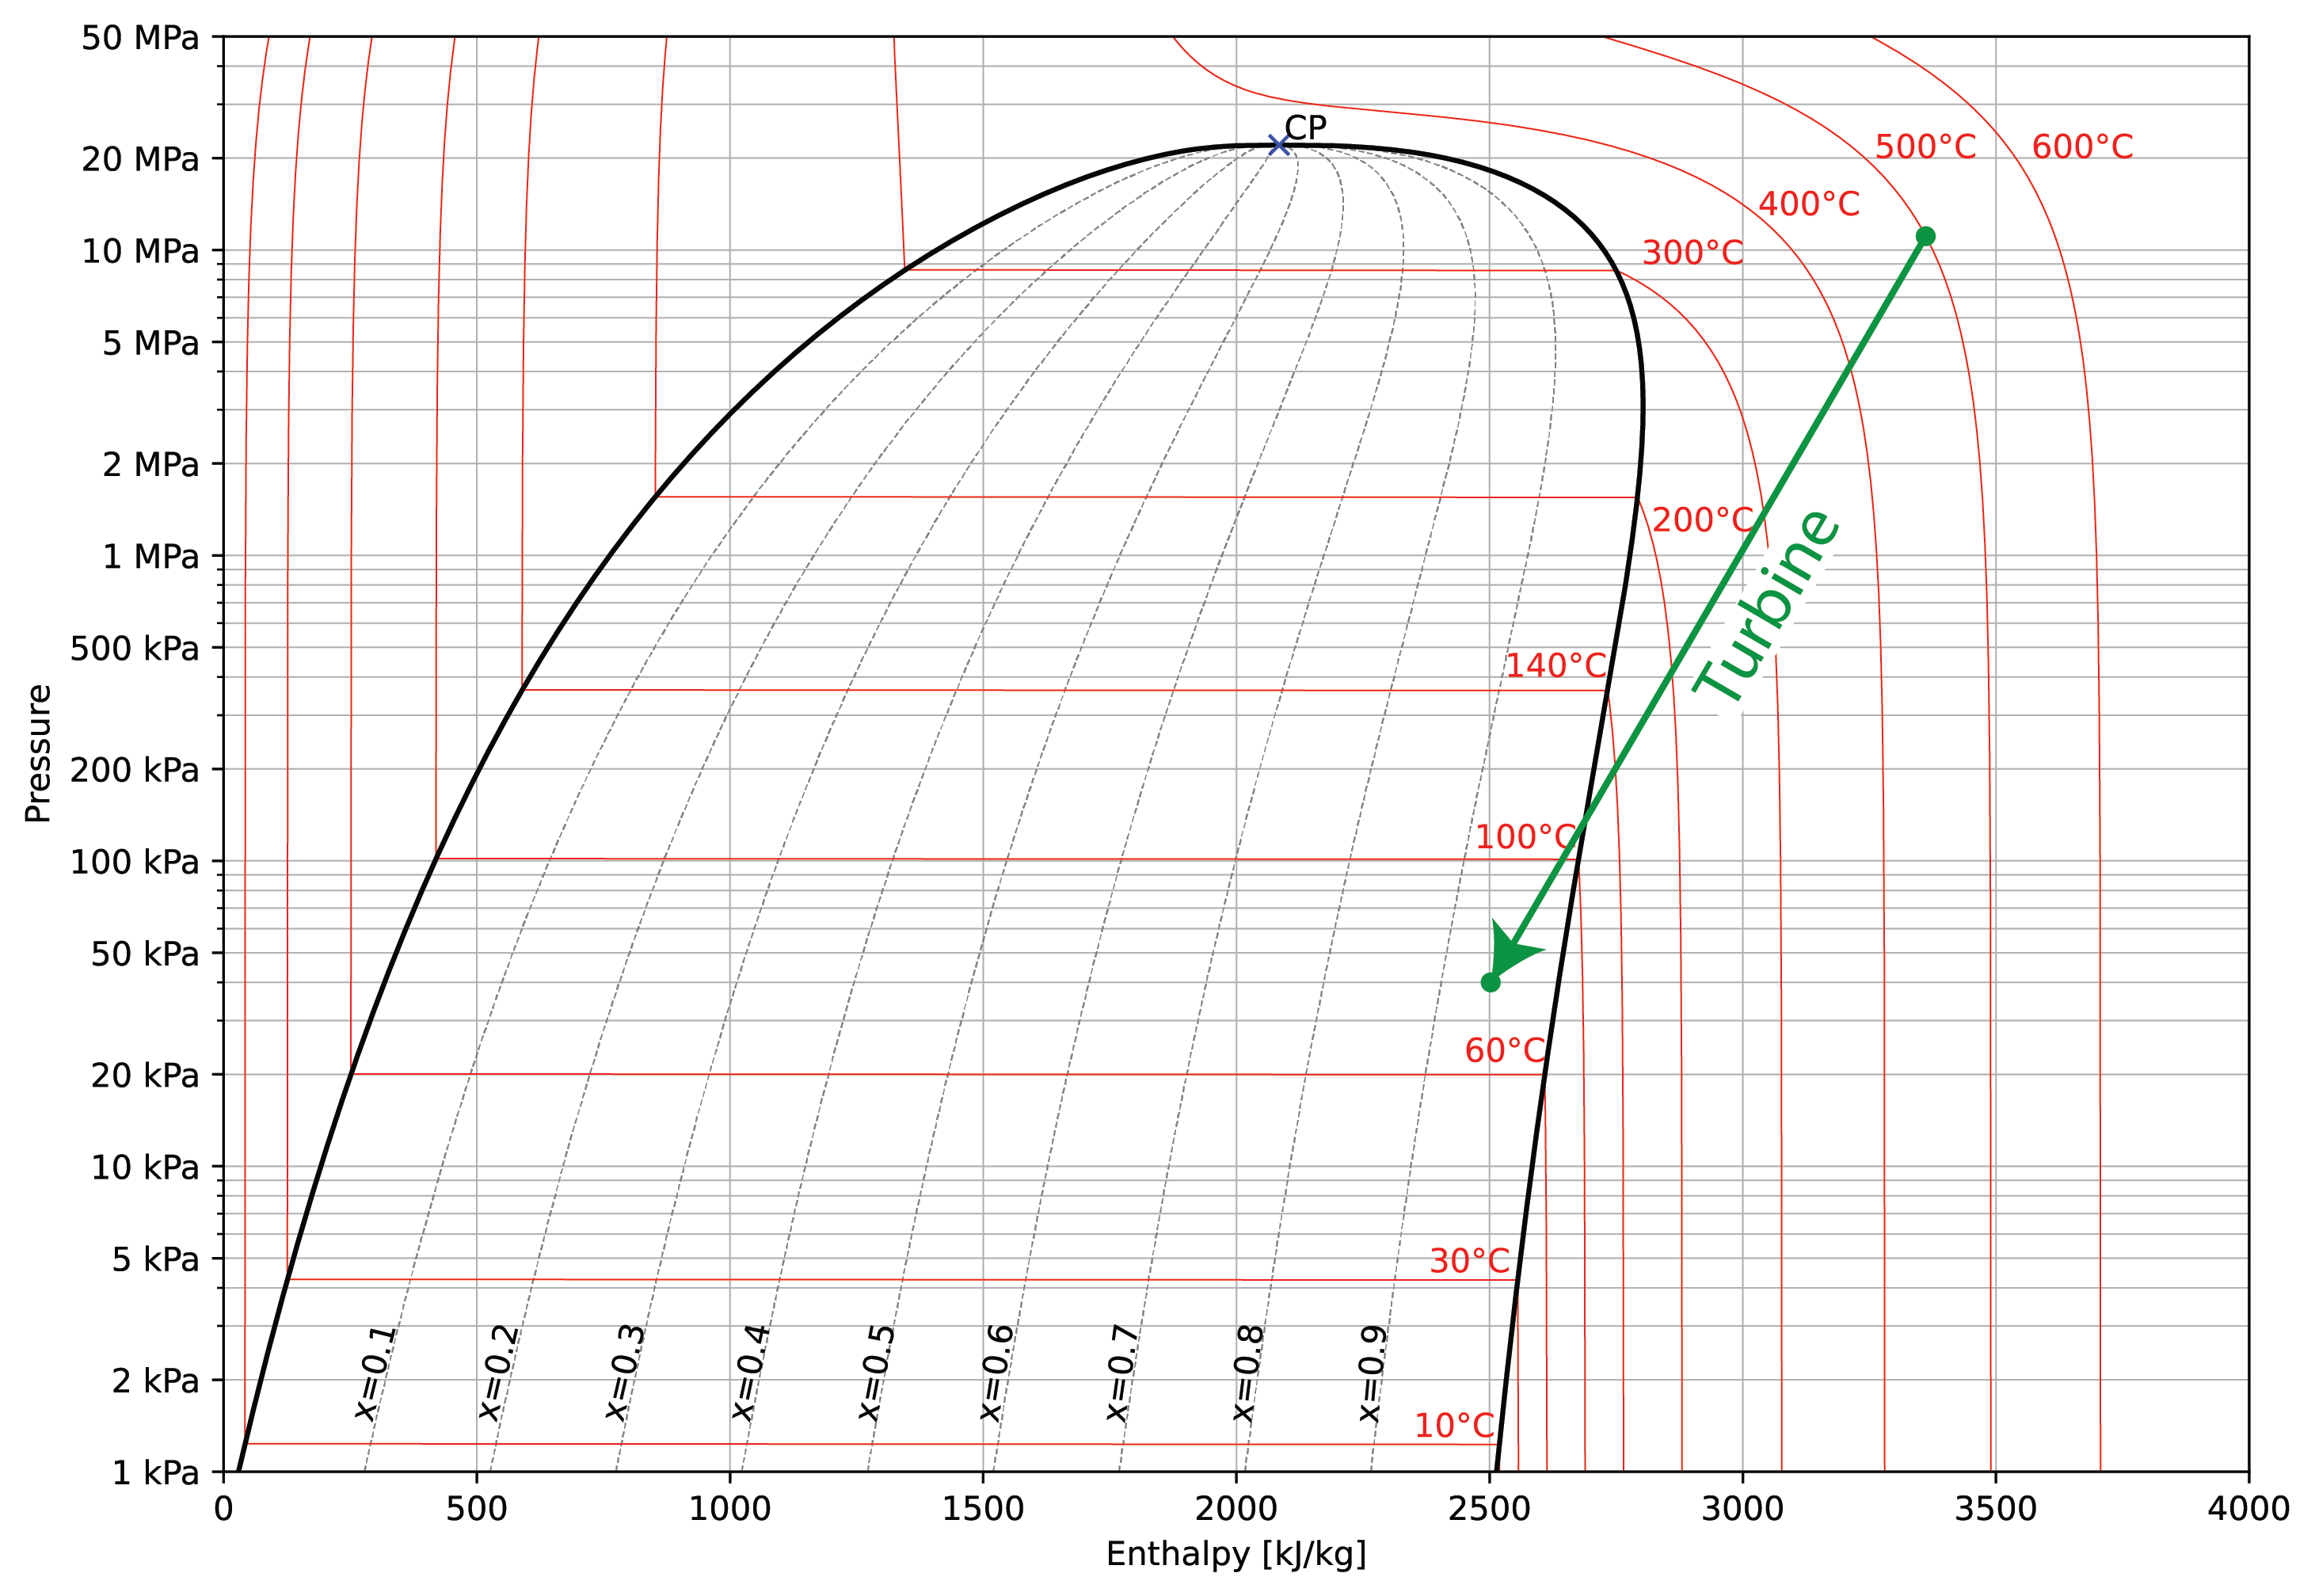
\includegraphics[width=0.75\textwidth]{Turbineph}
\caption{Typical turbine process plotted on a $p$-$h$ diagram for steam.}
\label{fig:ch4_turbineph}
\end{figure}

Within a turbine, you should expect the pressure, enthalpy, and temperature to decrease while the specific volume increases.  For a well designed steam turbine, the flow should start superheated or supercritical, and end either as saturated steam or as a gas-liquid mixture with a quality of at least 90\%.  If the quality drops too low, the large number of water droplets will begin to erode the turbine blades.


Figure \ref{fig:ch4_turbineph} shows a turbine process on a $p$-$h$ diagram, which highlights the drop in pressure and enthalpy, as well as the final state of water being at a fairly high quality.  In Example \ref{ex:ch4_supercrit}, we will see a Rankine cycle with two separate turbines.  In modern power plants, the turbine is often subdivided even further to account for high temperature steam being bled off for various purposes.  This can be seen in Example \ref{ex:ch4FeedwaterHeater}, in which some of the steam is used to preheat the water before boiling.

% --------------------------------------------------------------------
\subsection{Compressors and Pumps} \label{sec:ch4_pumps}

Compressors and pumps both act to add energy to a fluid through work.  The primary difference is that pumps act on liquids, while compressors work on gases.  Compressors and pumps come in many forms, varying from rotary compressors that look like the turbine in Figure \ref{fig:ch4_turbineDiagram} (though usually smaller) to reciprocating pumps that use pistons driven by a crankshaft, along with many other varieties.


\begin{figure}[H]
  \centering
  \begin{subfigure}[b]{0.3\textwidth}
    \centering
    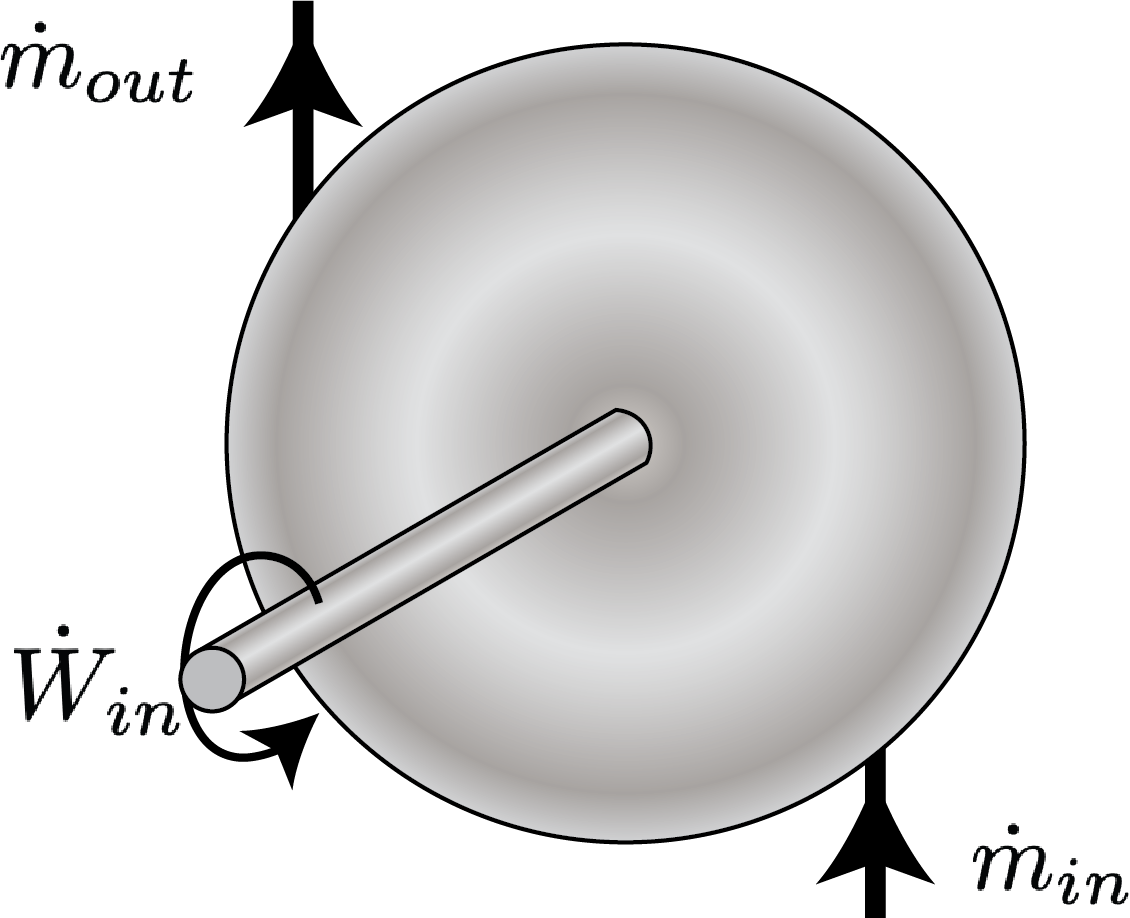
\includegraphics[width=1.0\textwidth]{PumpDiagram}
   
  \end{subfigure}
  \hspace{1 in}
  \begin{subfigure}[b]{0.3\textwidth}
    \centering
    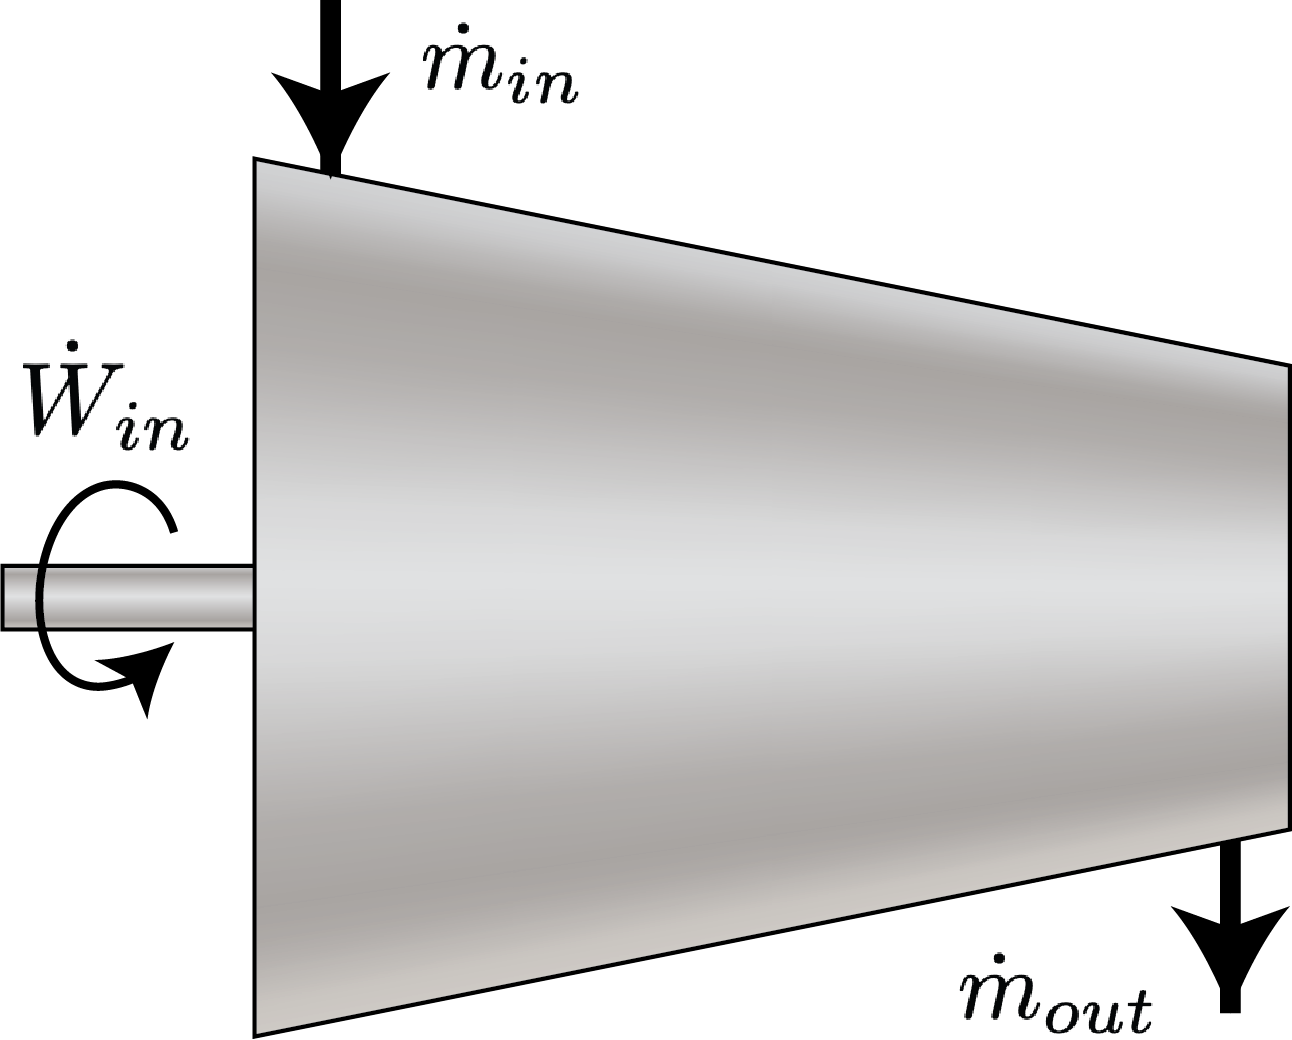
\includegraphics[width=1.0\textwidth]{CompressorDiagram}
  \end{subfigure}
   \caption{Left: Pump in for cycle diagrams. Right: Compressor in for cycle diagrams.}
\label{fig:ch4_compressorDiagram}
\end{figure}

\begin{figure}[H]
\centering
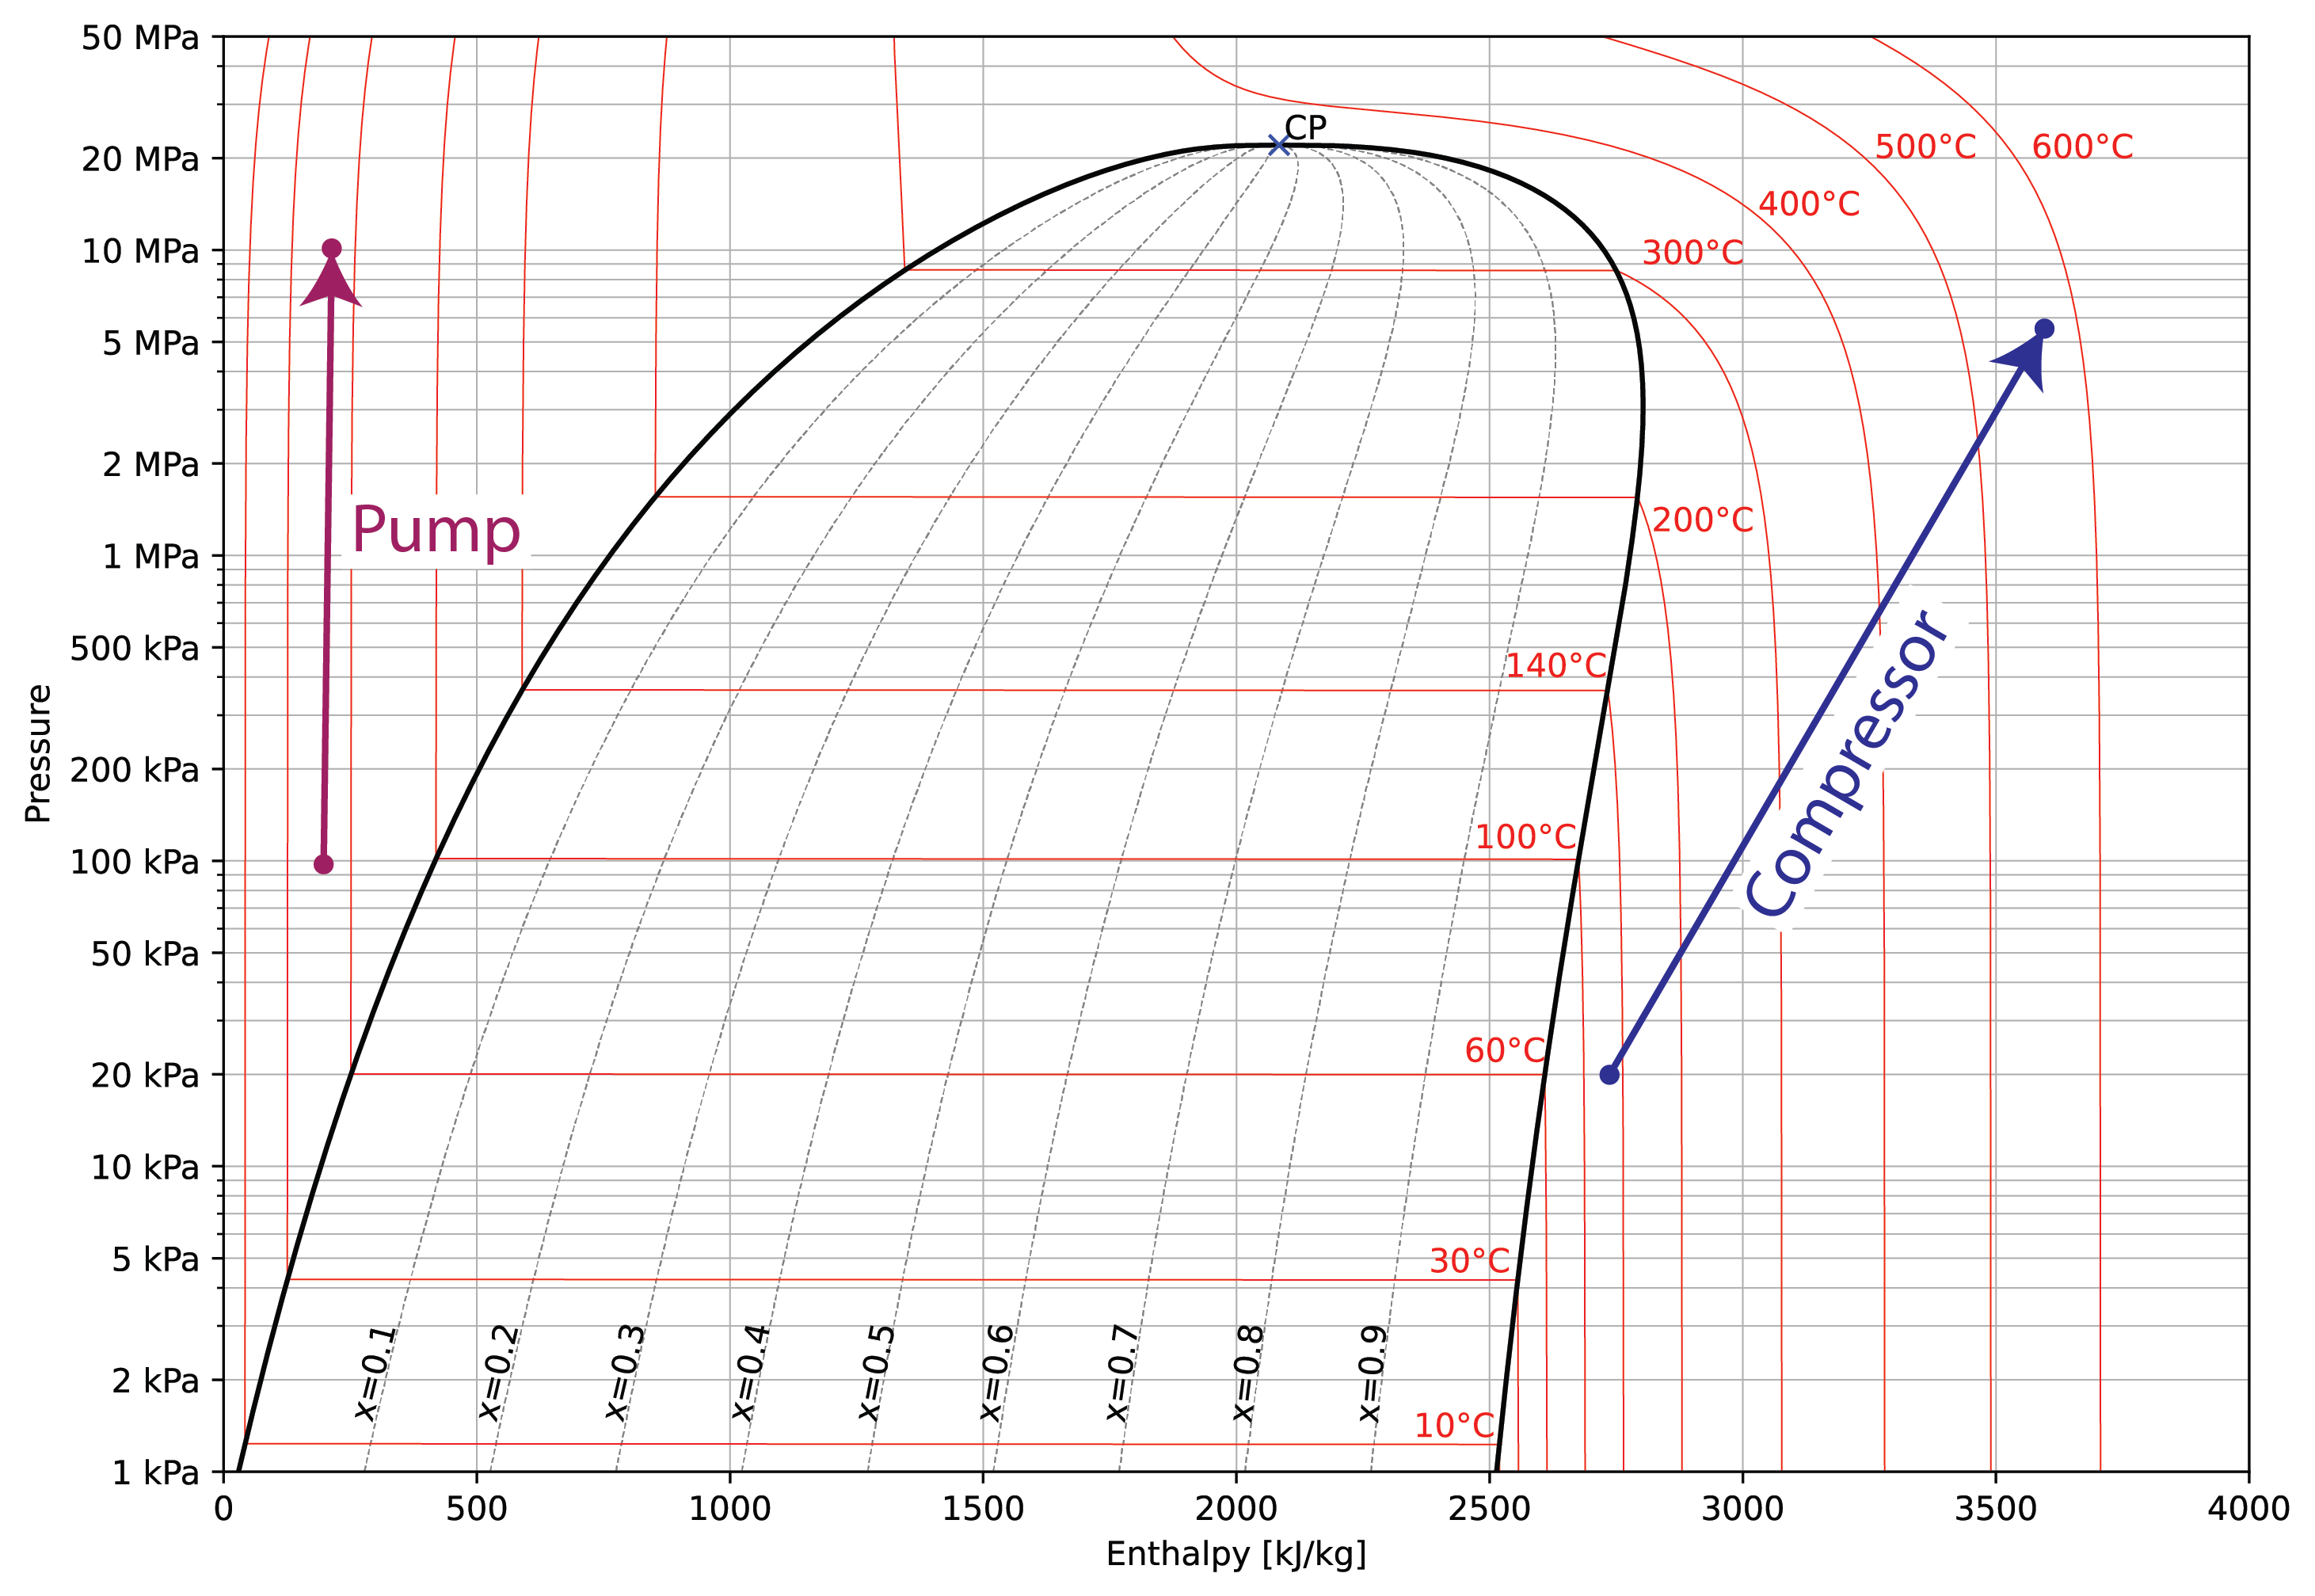
\includegraphics[width=0.75\textwidth]{Compressorph}
\caption{Typical compressor and pump processes plotted on a $p$-$h$ diagram for steam.}
\label{fig:ch4_compressorph}
\end{figure}

Thermodynamically, compressors are nearly the opposite of turbines, as can be seen by comparing Figures \ref{fig:ch4_turbineph} and \ref{fig:ch4_compressorph}.  Pressure, enthalpy, and temperature all increase through the compressor, while specific volume decreases.  One note is that compressors typically operate only in the superheated and supercritical regimes.  In other words, droplets of liquid, as are present in the quality region, are typically worse for compressors than they are for turbines.


Pumps operate in liquids, which are usually modeled as incompressible.  The result of this is that the amount of enthalpy change over a pump is very small compared to compressors.  In fact, we can often neglect the energy requirements of the pump in our analysis, and expect less that 1\% error in our final results.  An example pump is also shown in Figure \ref{fig:ch4_compressorph}.  If we do choose to calculate the enthalpy change in the pump, we can expand $\Delta h$ as follows:
\begin{align}
  \nonumber \Delta h &= \Delta u + \Delta (pv) \\
  \nonumber \Delta h &= c \cancelto{0}{\Delta T} + p\cancelto{0}{\Delta v} + v\Delta p \\
\label{eq:ch4_pumpEnthalpy} \Delta h &= v\Delta p
\end{align}

The temperature change $\Delta T$ is assumed small, and the change in specific volume can be removed by assuming liquid water is incompressible.  The only remaining term occurs due to the change in pressure with constant volume.

Like compressors, pumps should not operate in the quality region.  Whereas droplets of water can cause erosion of the compressor machinery, bubbles of steam can occur as cavitation, which cause significantly more serious pressure spikes that can damage or destroy pump machinery.

% --------------------------------------------------------------------
\subsection{Boilers, Evaporators, and Steam Generators}  \label{sec:ch4_boilers}

\begin{figure}[H]
  \centering
  \begin{subfigure}[b]{0.55\textwidth}
    \centering
    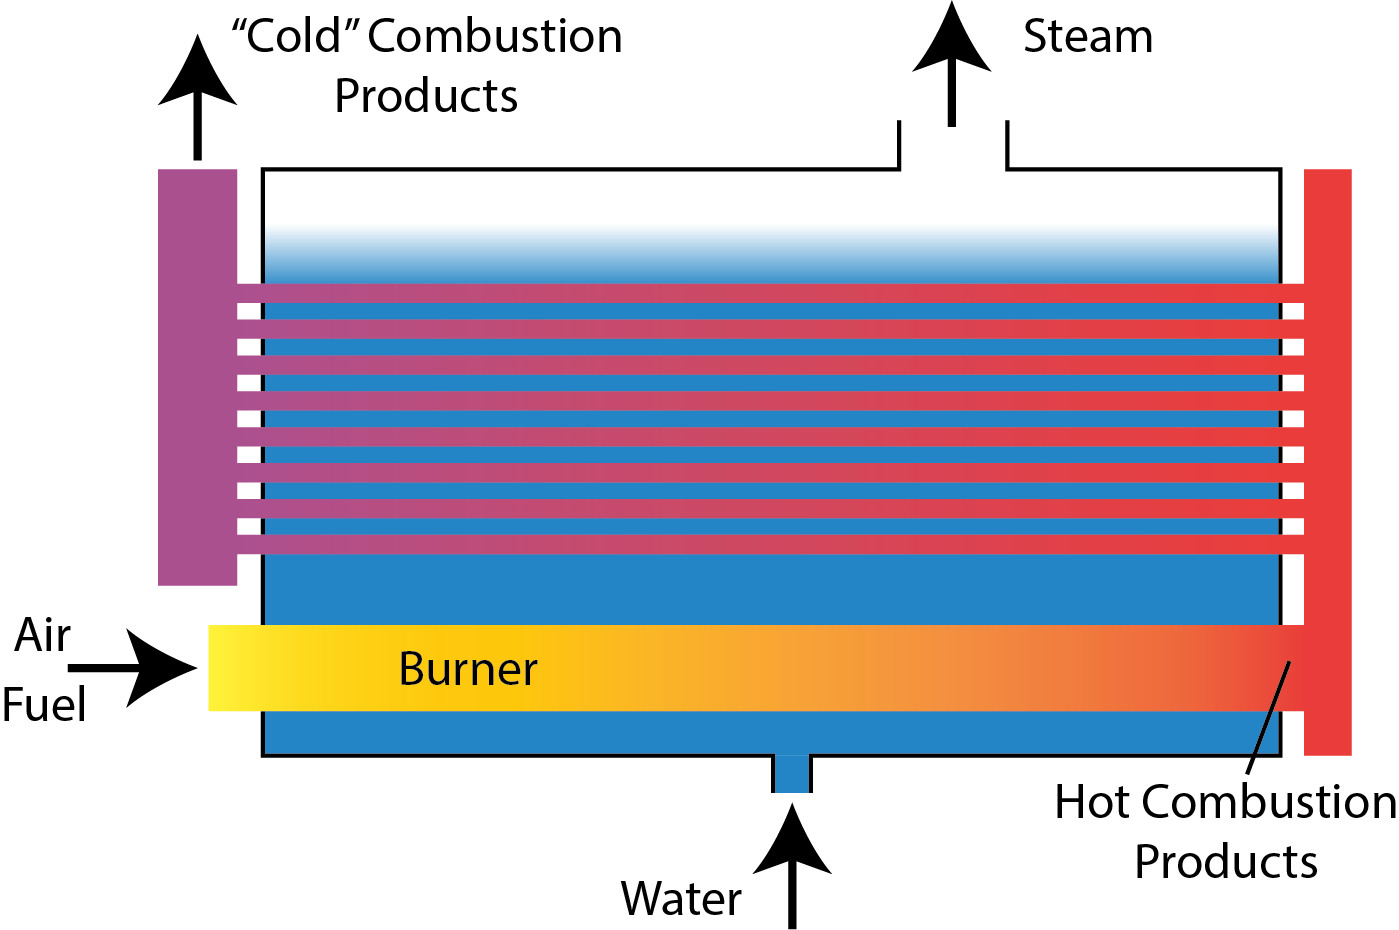
\includegraphics[width=1.0\textwidth]{BoilerDiagram}
   
  \end{subfigure}
  \hfill
  \begin{subfigure}[b]{0.42\textwidth}
    \centering
    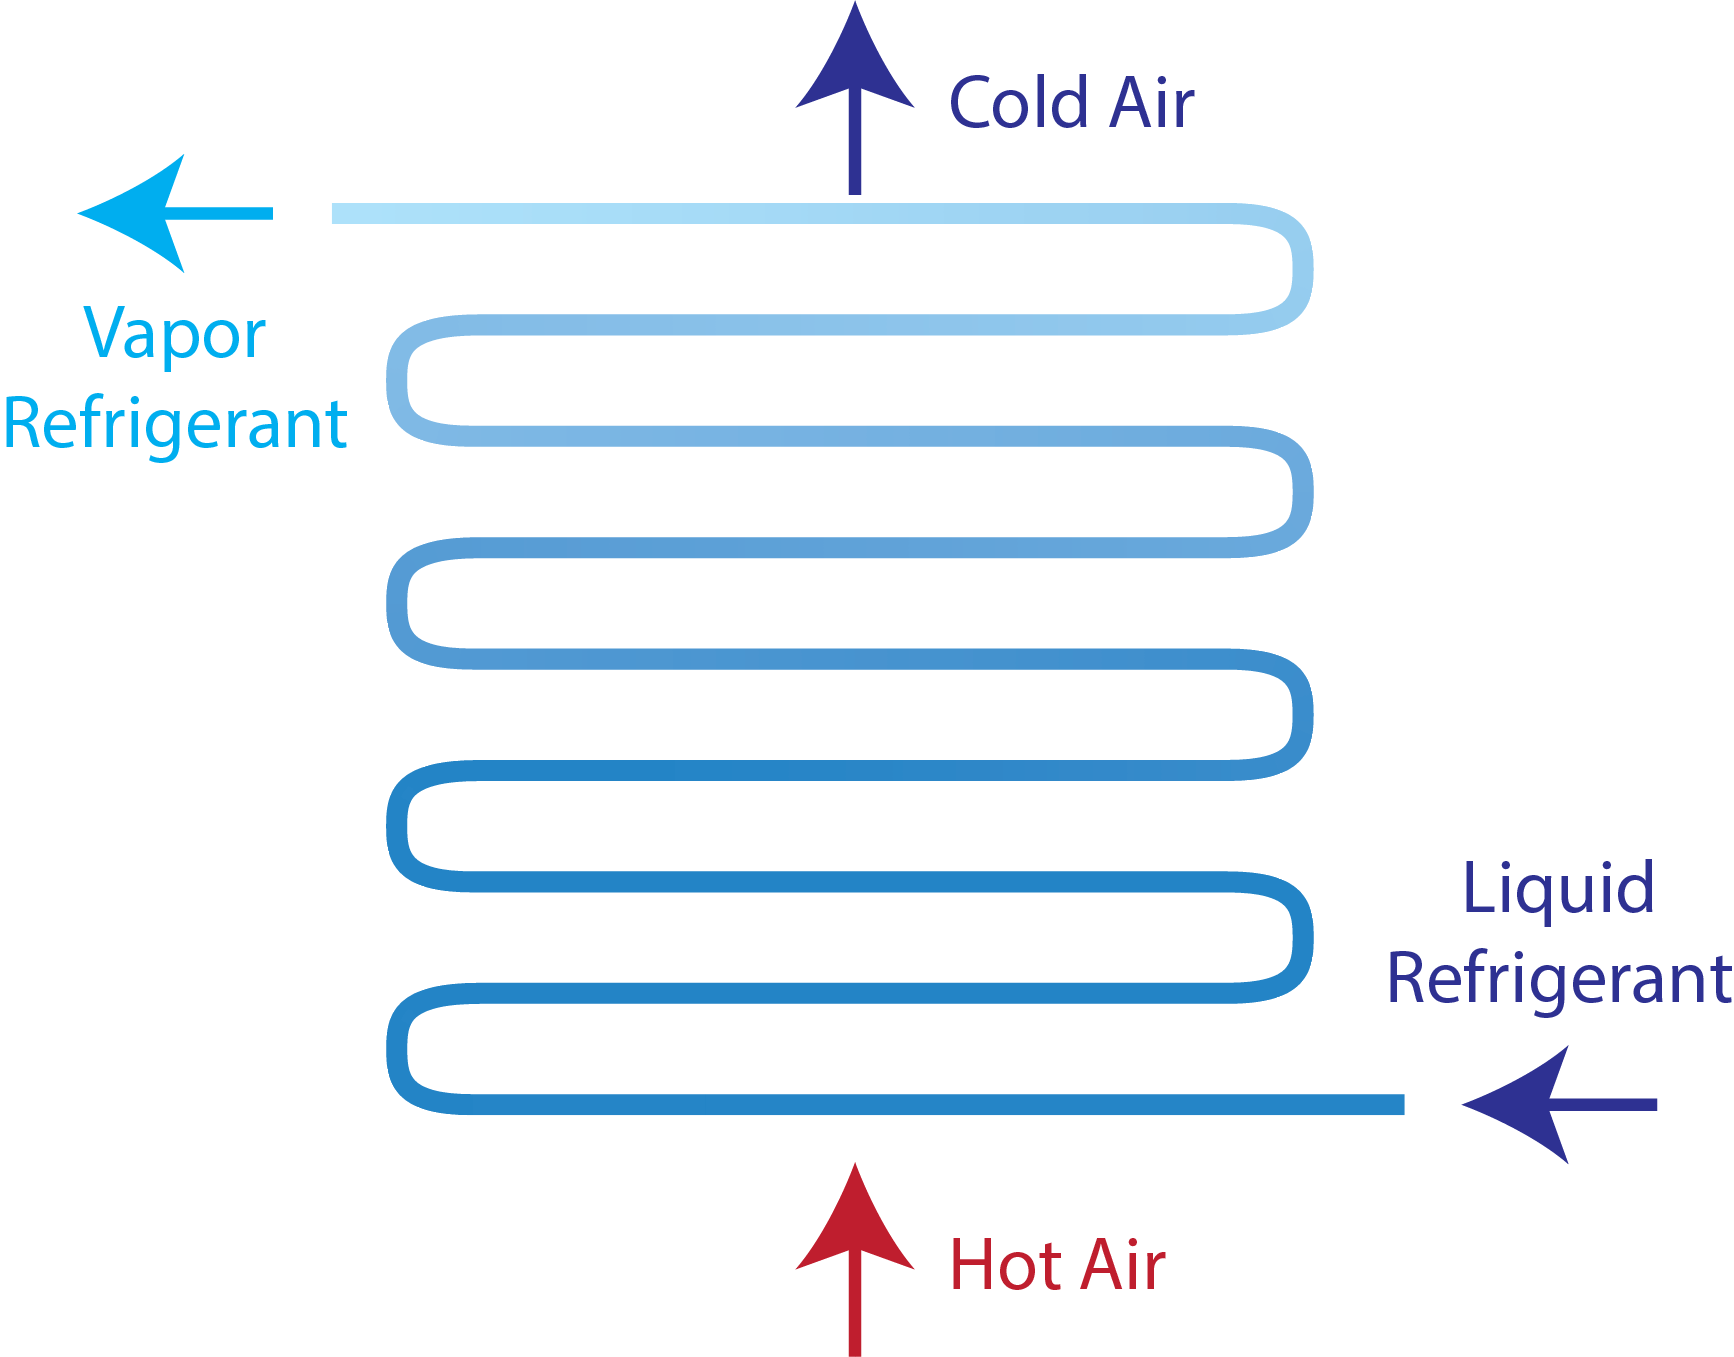
\includegraphics[width=1.0\textwidth]{EvaporatorDiagram}
  \end{subfigure}
   \caption{Left: Gas fired boiler, showing the inflow and burning of fuel and gas, the cooling of combustion products as the heat is transferred to the water, and the conversion of water into steam. Right: Evaporator, showing the flow of refrigerant as it evaporates inside the pipes, as well as the air flowing outside of the pipes.}
\label{fig:ch4_boilerDiagram}
\end{figure}

Boilers, evaporators, and steam generators all add heat to a fluid, and the end result is a gas, as shown in Figure \ref{fig:ch4_boilerph}.  Boilers and steam generators both add heat at elevated pressure.  A boiler adds heat to a compressed liquid, changing its phase to steam through the vapor envelope.  Steam generators do not literally boil the liquid, as the starting point is water at supercritical pressure.  As heat is added, the vapor envelope is avoided completely, and the end result is supercritical vapor.

\begin{figure}[H]
\centering
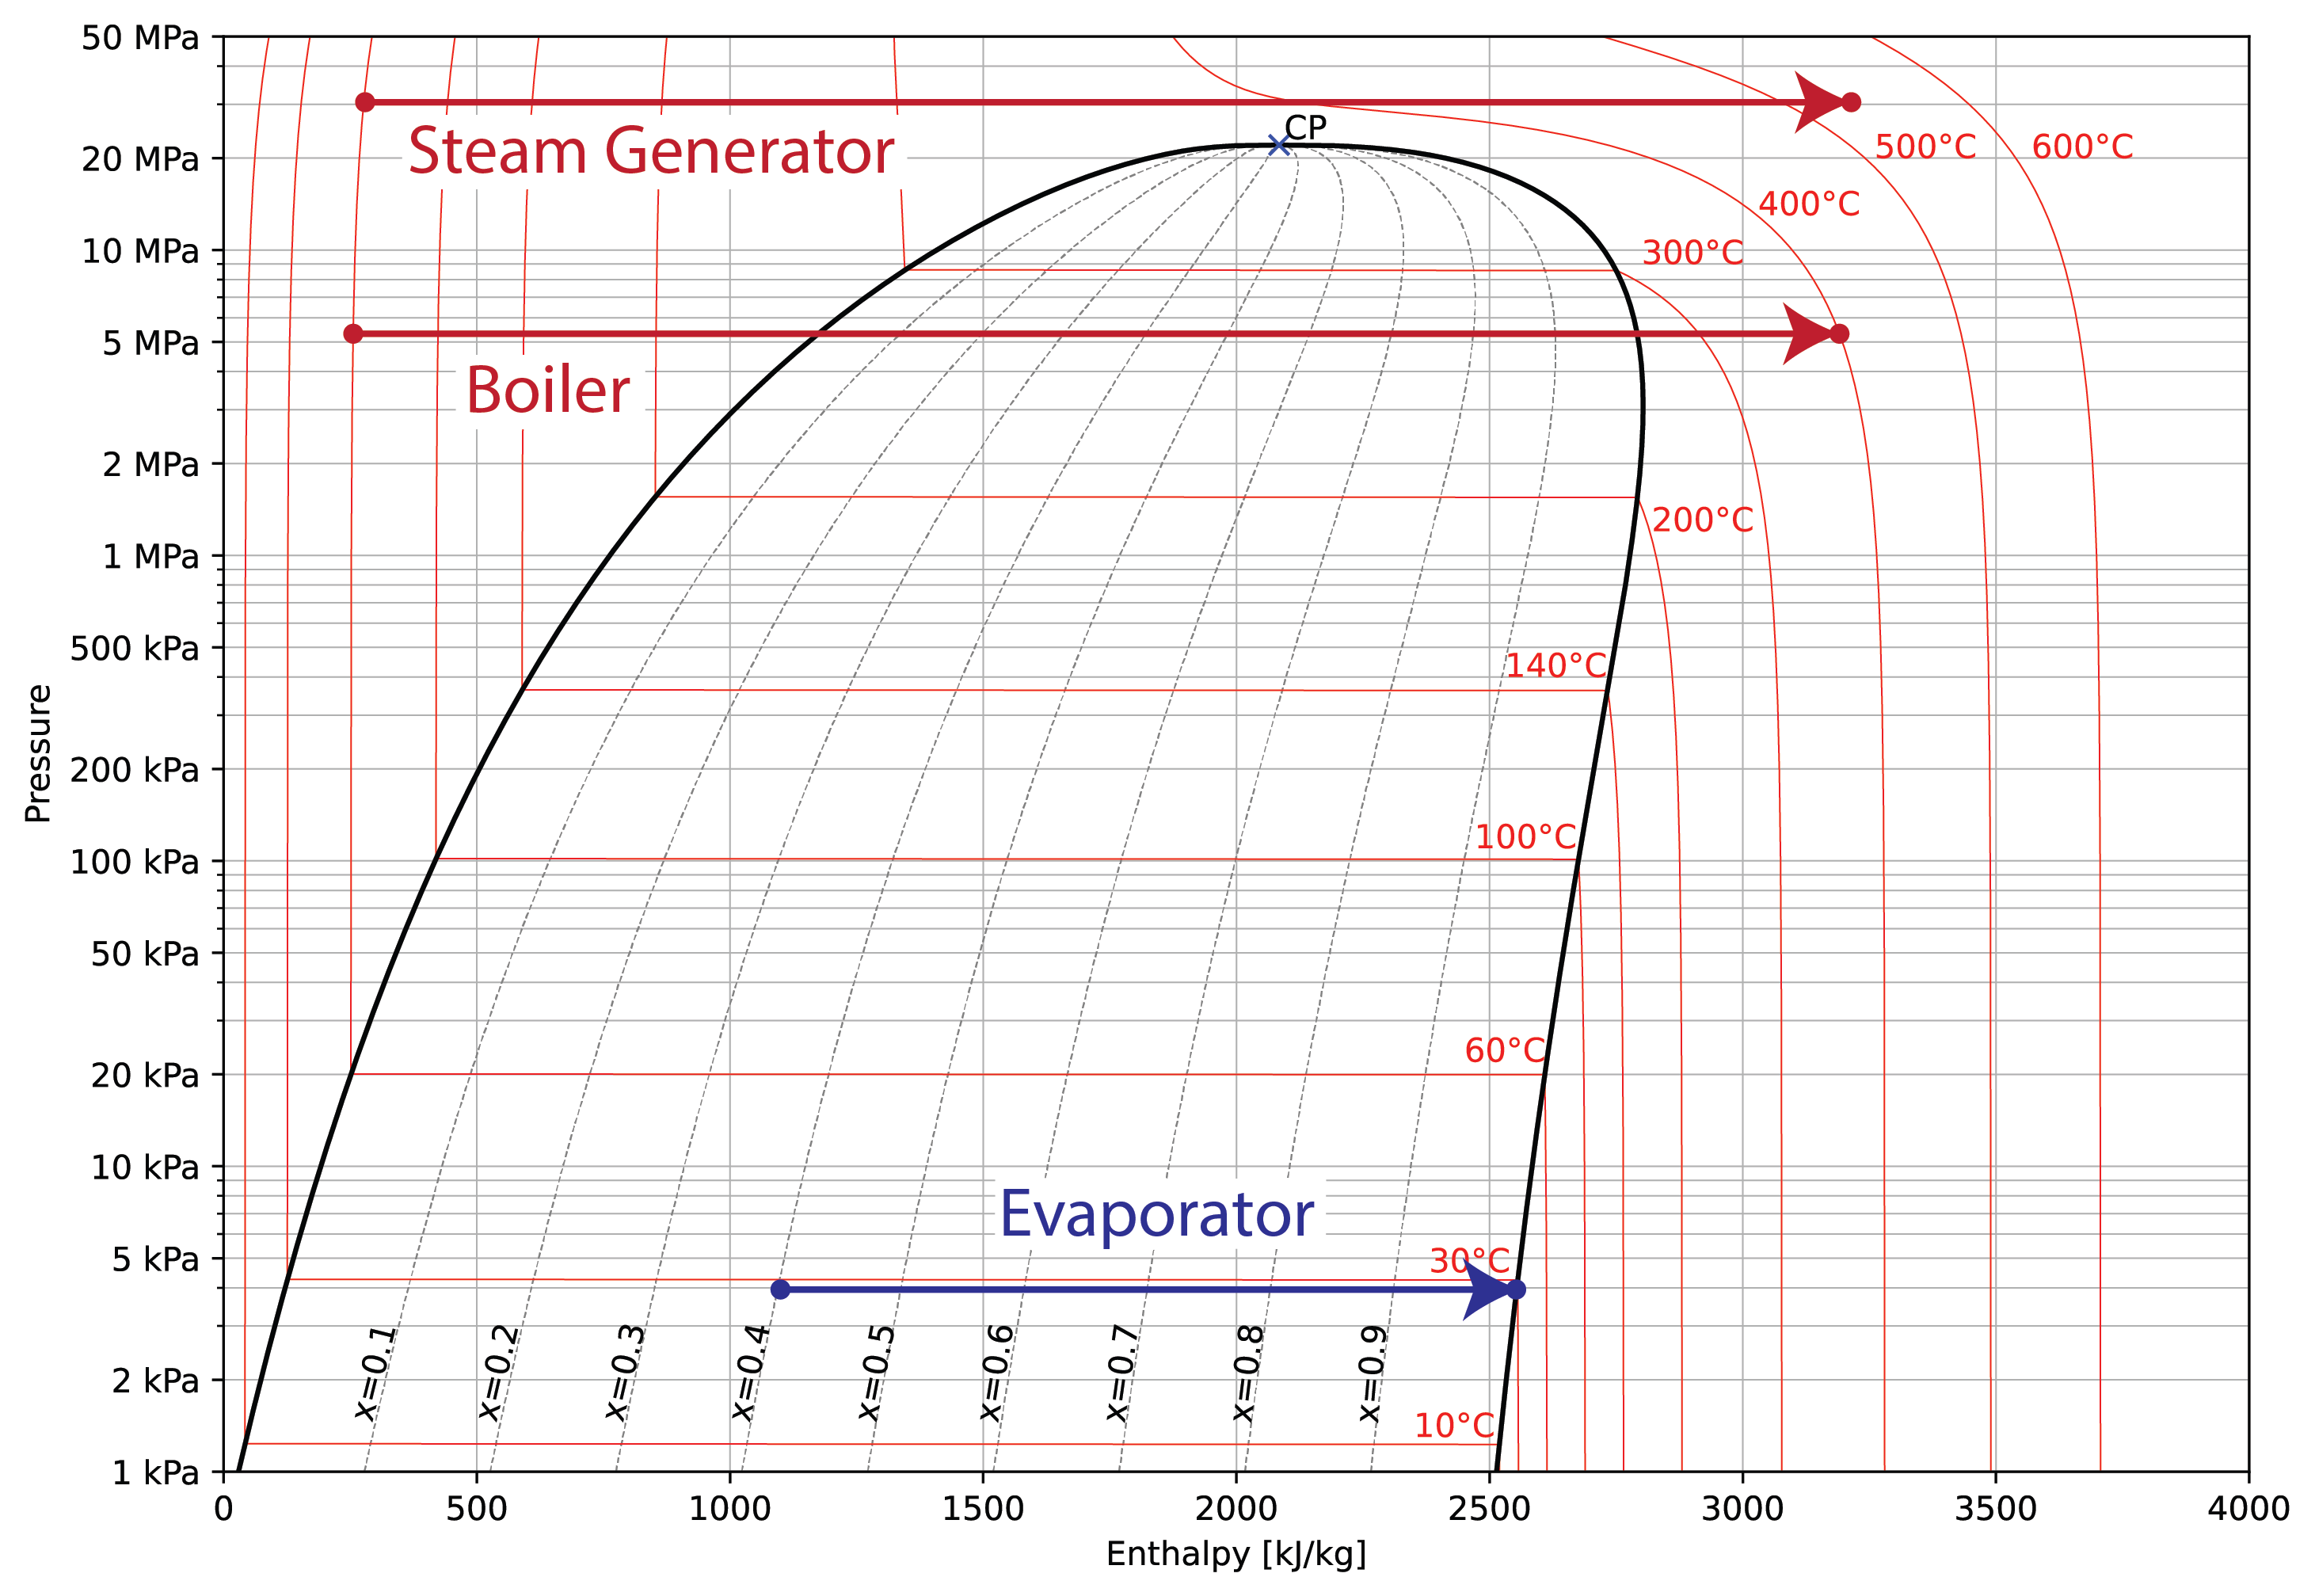
\includegraphics[width=0.75\textwidth]{Boilerph}
\caption{Typical boiler, evaporator, and steam generator processes plotted on a $p$-$h$ diagram for steam.}
\label{fig:ch4_boilerph}
\end{figure}

Evaporators typically operate at lower pressure and temperature, and find use in HVAC (air conditioning) units.  In this class, we will see evaporators using R134a, though they are used for water in the food industry (concentration of juices, for instance).

In all three cases, the pressure is assumed to remain constant while the enthalpy increases.  In reality, there is typically a slight pressure decrease associated with friction in the fluid flow, but this is neglected in this class.
% --------------------------------------------------------------------
\subsection{Condensers}  \label{sec:ch4_condensers}

A condenser is a type of heat exchanger in which heat is extracted from the steam or refrigerant in our system/cycle and sent into water or air outside of the system/cycle.

Like boilers and evaporators, the pressure is assumed to remain constant through a condenser, while the enthalpy drops drastically.  For power plants, condensation occurs at relatively low temperatures, while for air conditioning units, condensation occurs at relatively high temperatures.  Both are shown in Figure \ref{fig:ch4_condenserph}.

\begin{figure}[H]
\centering
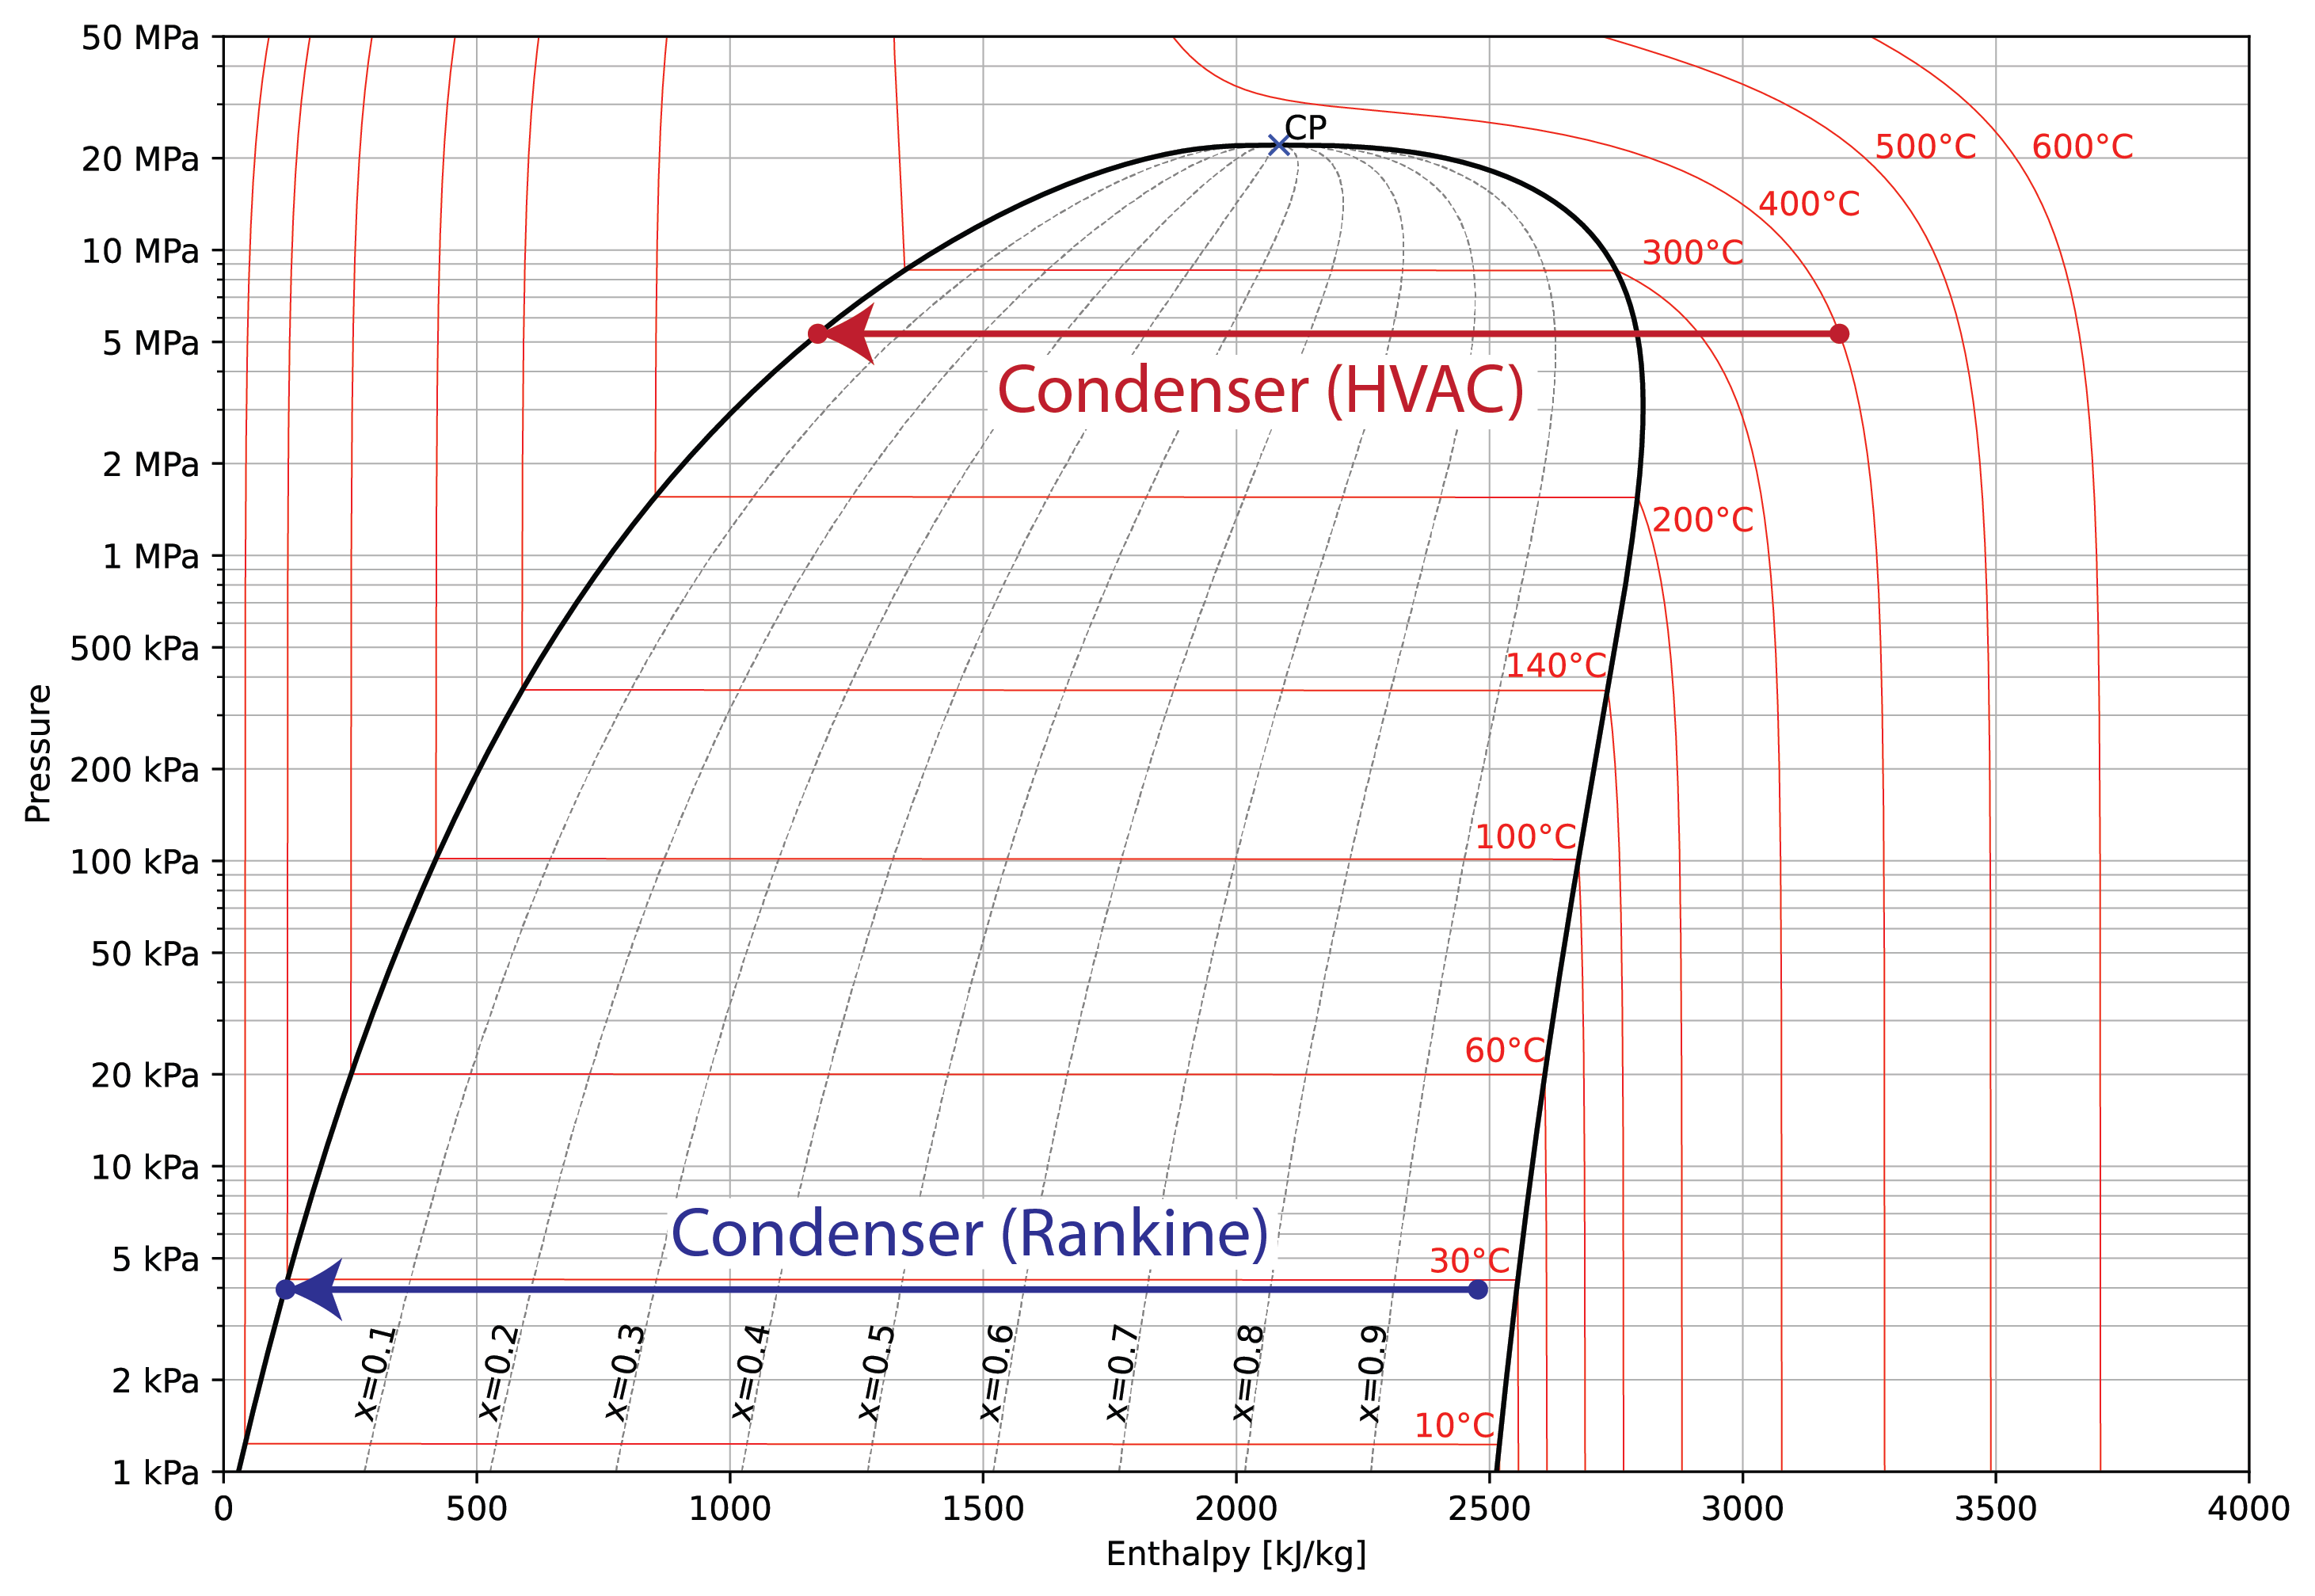
\includegraphics[width=0.75\textwidth]{Condenserph}
\caption{Typical condenser processes for power plants and air conditioning units plotted on a $p$-$h$ diagram for steam.}
\label{fig:ch4_condenserph}
\end{figure}

Condensers in power plants typically consist of many small pipes containing cold water, with steam flowing over the pipes while cooling and condensing.  The cold water heats up, and the steam condenses back to liquid water.  Condensers therefore require a constant supply of cold water, typically from a nearby river or lake.  The amount of water required can be reduced through the use of a cooling tower, which uses evaporative cooling to extract large amount of energy.

Condensers for HVAC applications are normally a single pipe containing the refrigerant, over which air is blown.  Because of the high pressure of the refrigerant in HVAC systems, the air is normally significantly cooler, which allows the refrigerant to condense in the pipe.  In essence, this works opposite from the evaporator shown in Figure \ref{fig:ch4_boilerDiagram}.
% --------------------------------------------------------------------
\subsection{Mixers}  \label{sec:ch4_mixers}
Mixers allow multiple streams of fluid to reunite as a single stream.  The output of a mixer is governed by the following equation:
\begin{equation} \label{eq:ch4_mixer}
  \dot{m}_{out} h_{out} = \sum \dot{m}_{in} h_{in}
\end{equation}
Equation \ref{eq:ch4_mixer} assumes that the mixing process requires no work and is adiabatic.

Open feedwater heaters are examples of mixers that are seen in more advanced power cycles.  A portion of the hot steam is siphoned off after some work has been extracted, and that steam is mixed with water after condensation.  The end result is that the water can be heated to near the boiling point, and less fuel is needed in the boiler.

%The $p$-$h$ diagram for a mixer is shown in Figure \ref{fig:ch4_mixerph}.  

\begin{figure}[H]
\centering
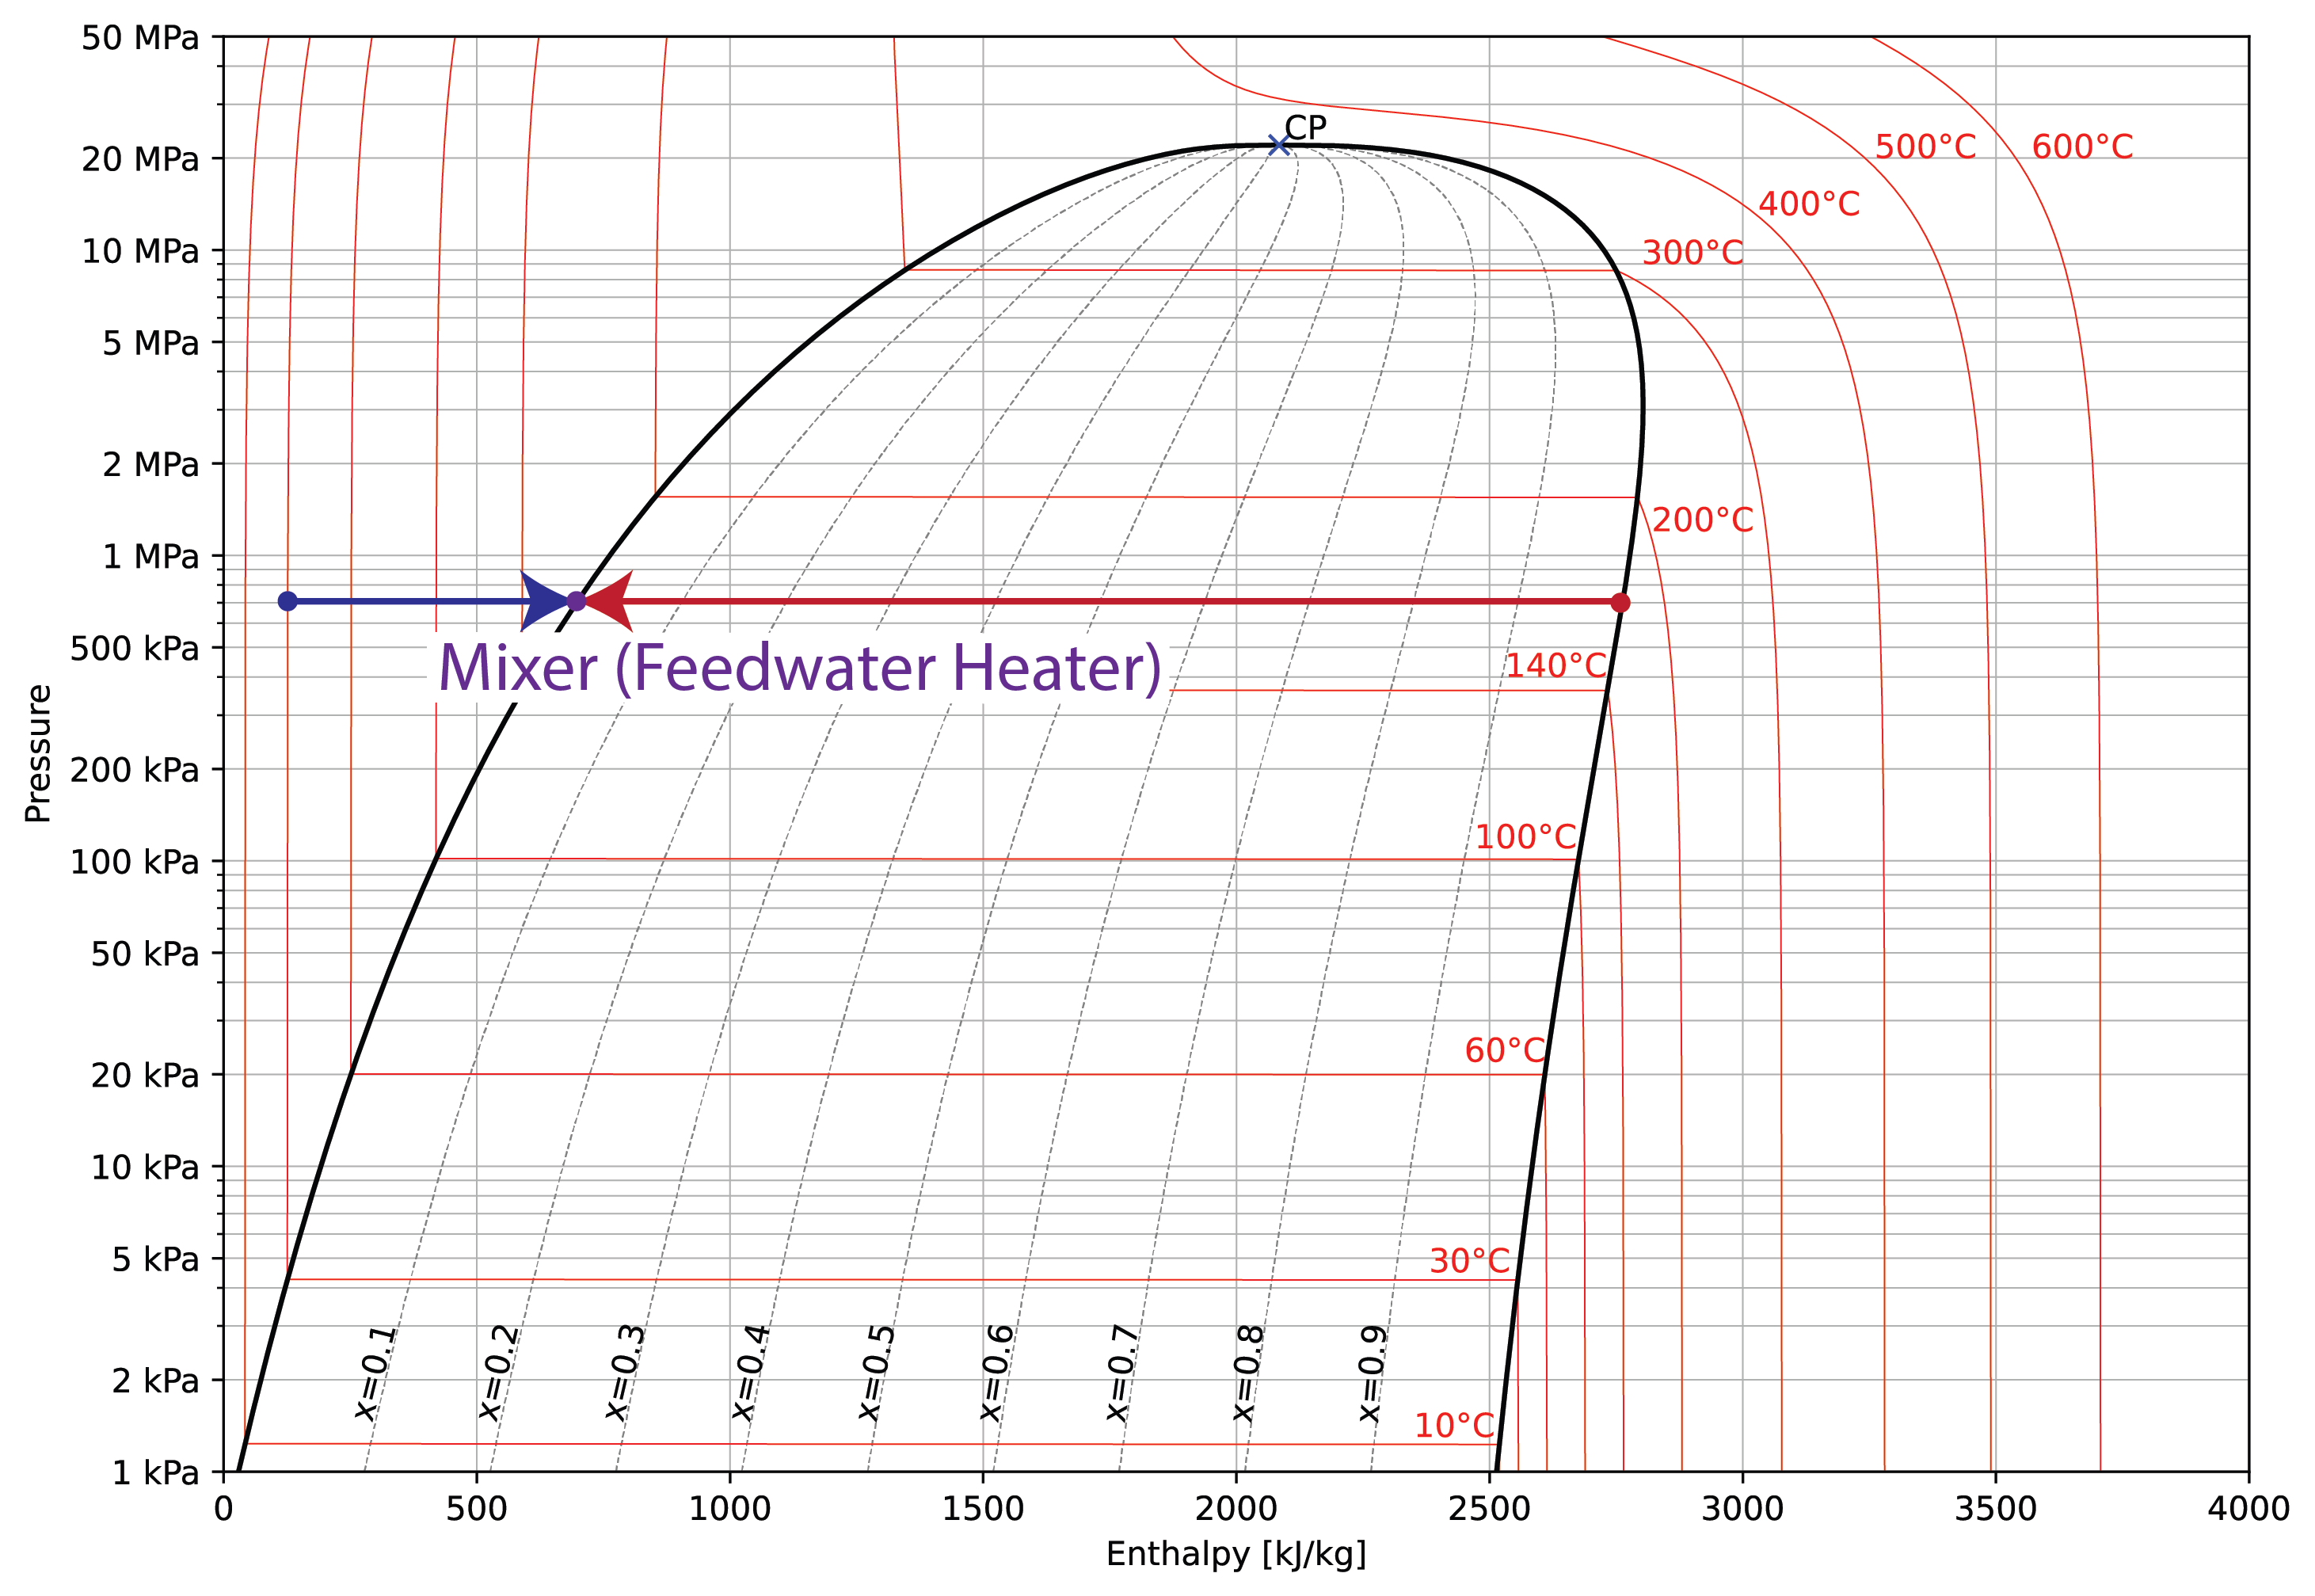
\includegraphics[width=0.75\textwidth]{Mixerph}
\caption{Typical mixer process plotted on a $p$-$h$ diagram for steam.}
\label{fig:ch4_mixerph}
\end{figure}
% --------------------------------------------------------------------
\subsection{Throttles}  \label{sec:ch4_throttles}
Throttles are components used primarily in HVAC systems.  They are able to reduce the pressure by changing mechanical energy to thermal energy through friction.  Essentially, they force the refrigerant to flow through very small holes or tubes to maximize the pressure loss.  In the HVAC profession, the throttle will be called a metering device, which could be either a capillary tube (typical for refrigerators) or an expansion valve (for residential A/C or more complex units).

\begin{figure}[H]
\centering
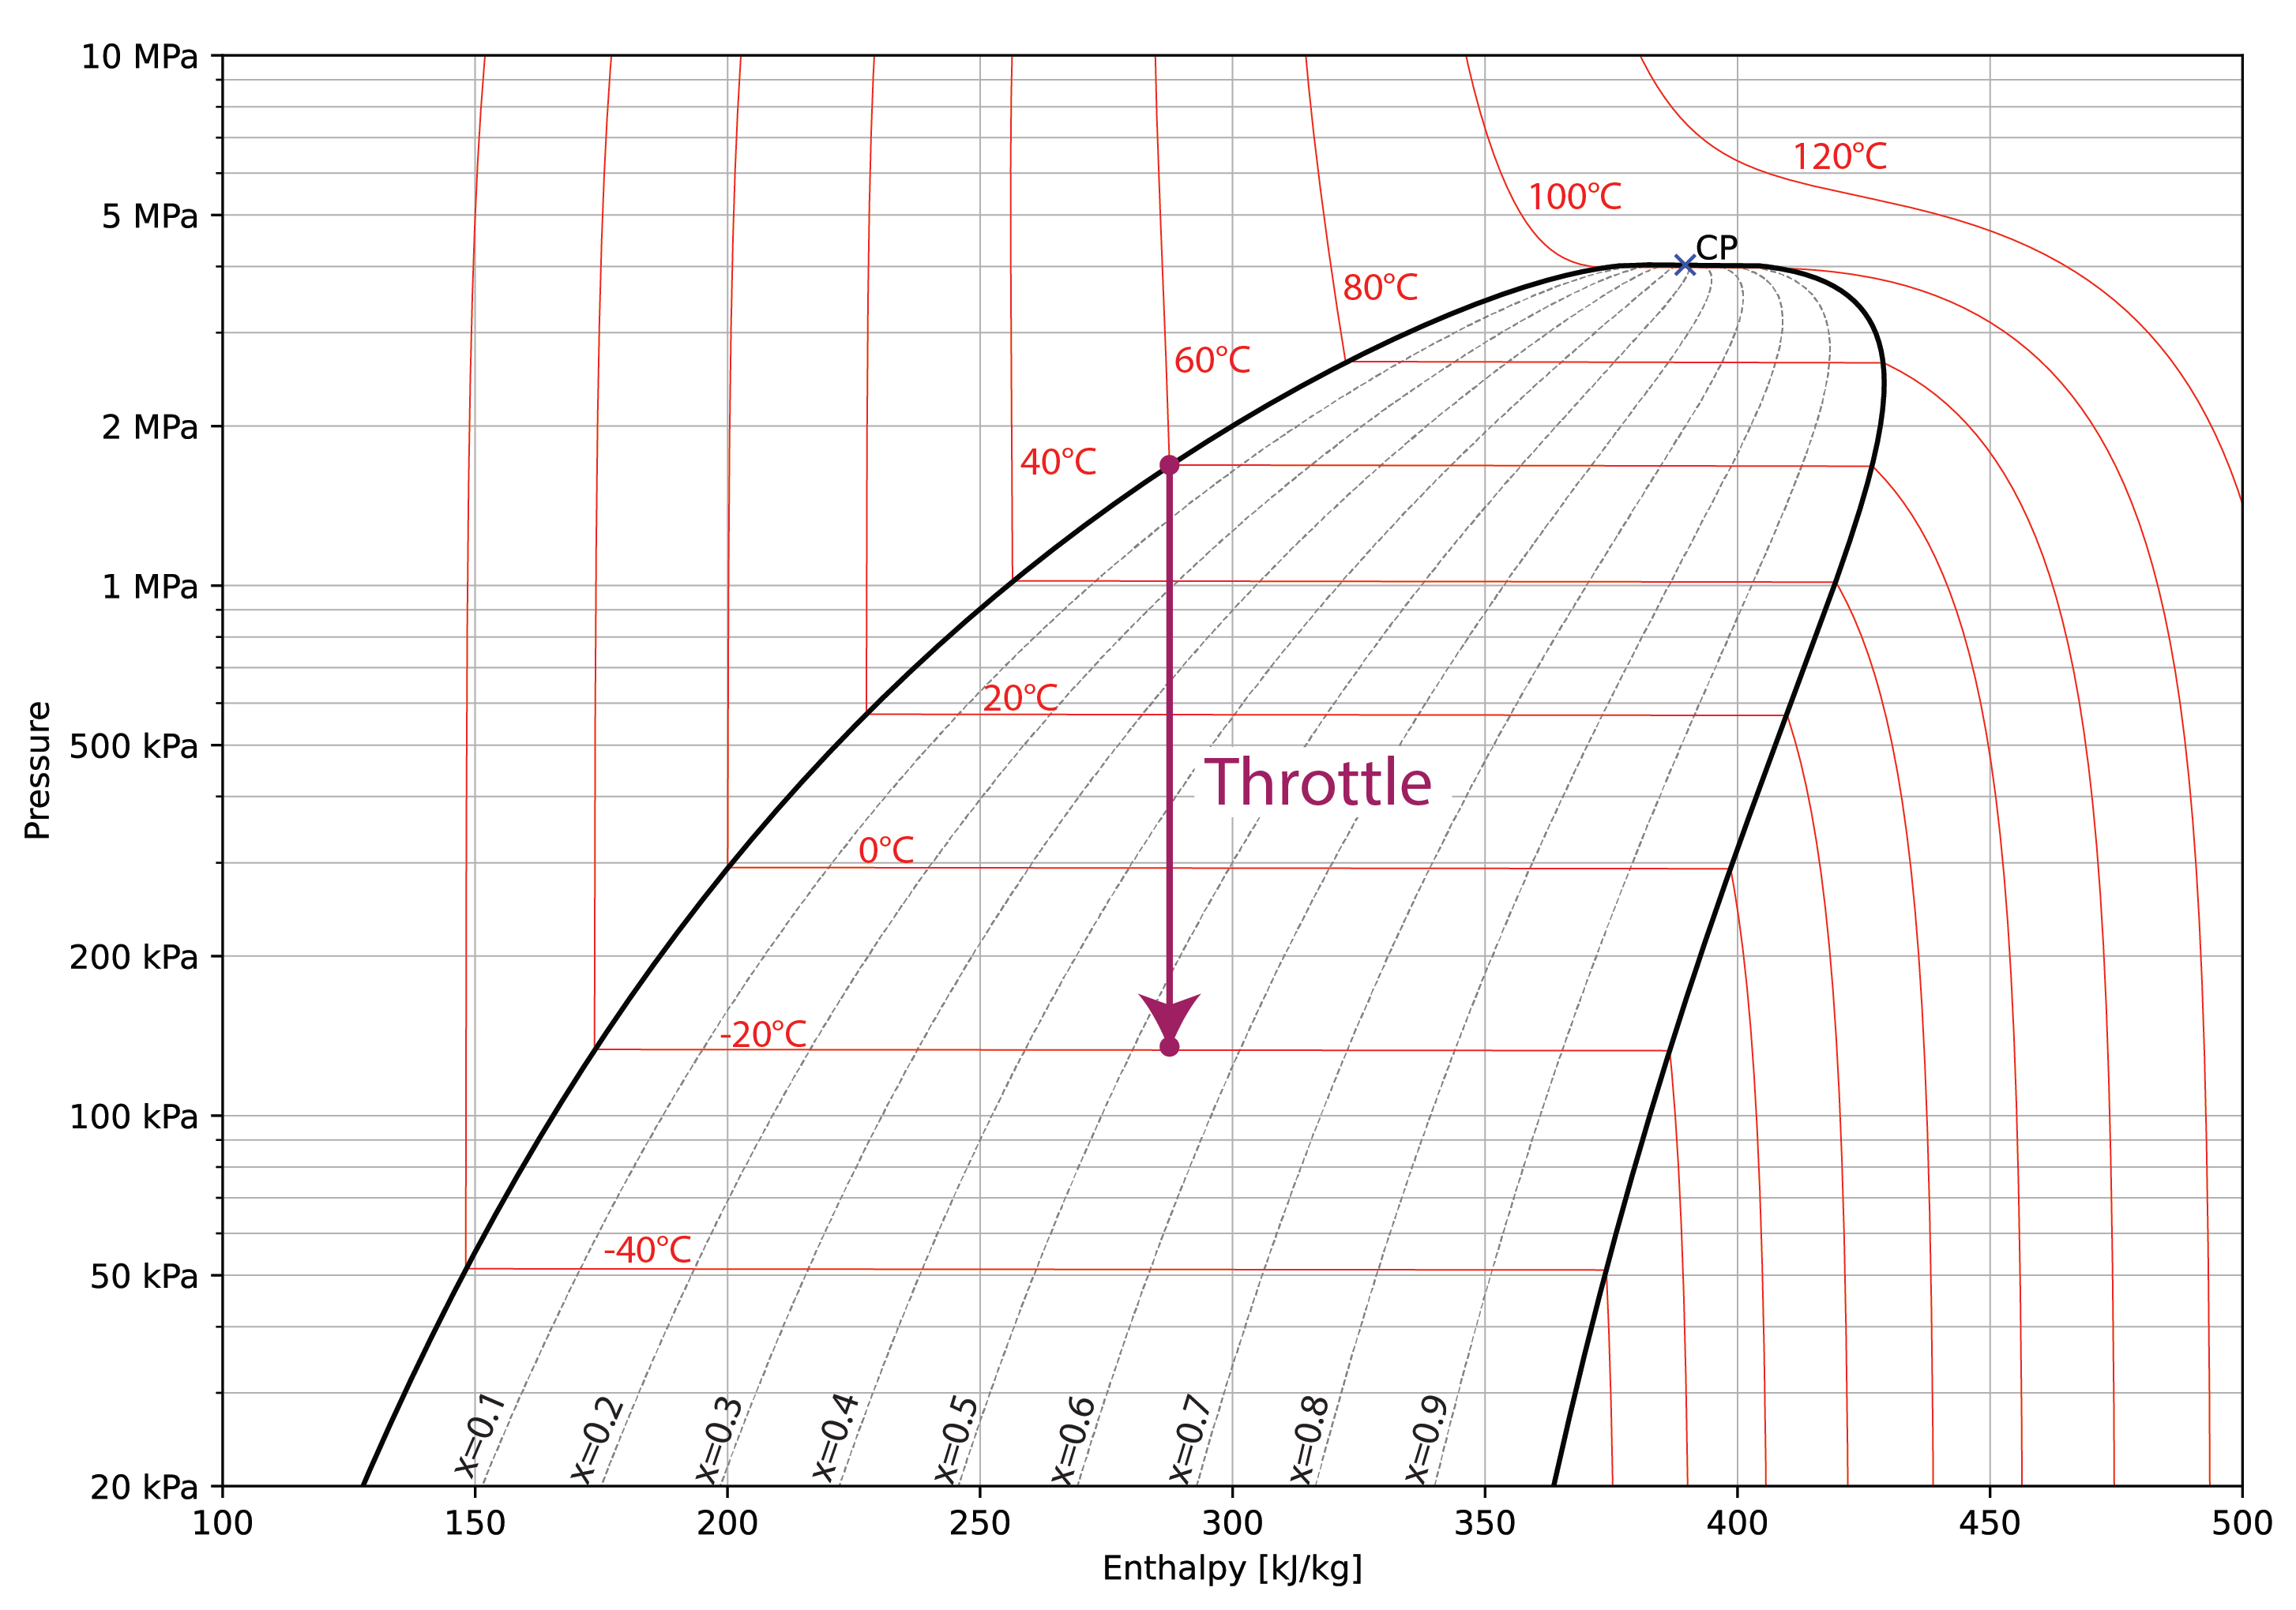
\includegraphics[width=0.75\textwidth]{Throttleph}
\caption{Typical throttle process plotted on a $p$-$h$ diagram for R-134a.}
\label{fig:ch4_throttleph}
\end{figure}

Throttles have no moving parts, and so cannot perform or extract any work.  Additionally, it is typically assumed that throttles are adiabatic.  Without any work or heat transfer, throttles cannot change the enthalpy in the flow.  That is, the throttling process is isenthalpic, or constant enthalpy, resulting in a vertical process in a $p$-$h$ diagram, as shown in Figure \ref{fig:ch4_throttleph}.
% --------------------------------------------------------------------
\subsection{Heat Exchangers}  \label{sec:ch4_heatExchangers}

Heat exchangers come in many shapes and sizes.  The key concept is bringing a hot fluid in close thermal contact to a cold fluid, and letting the heat naturally move from hot to cold.  As you can see in Figure \ref{fig:ch4_heatexchangerph}, the hot side of the heat exchanger is losing enthalpy, while the cold side is gaining it.  
\begin{figure}[H]
\centering
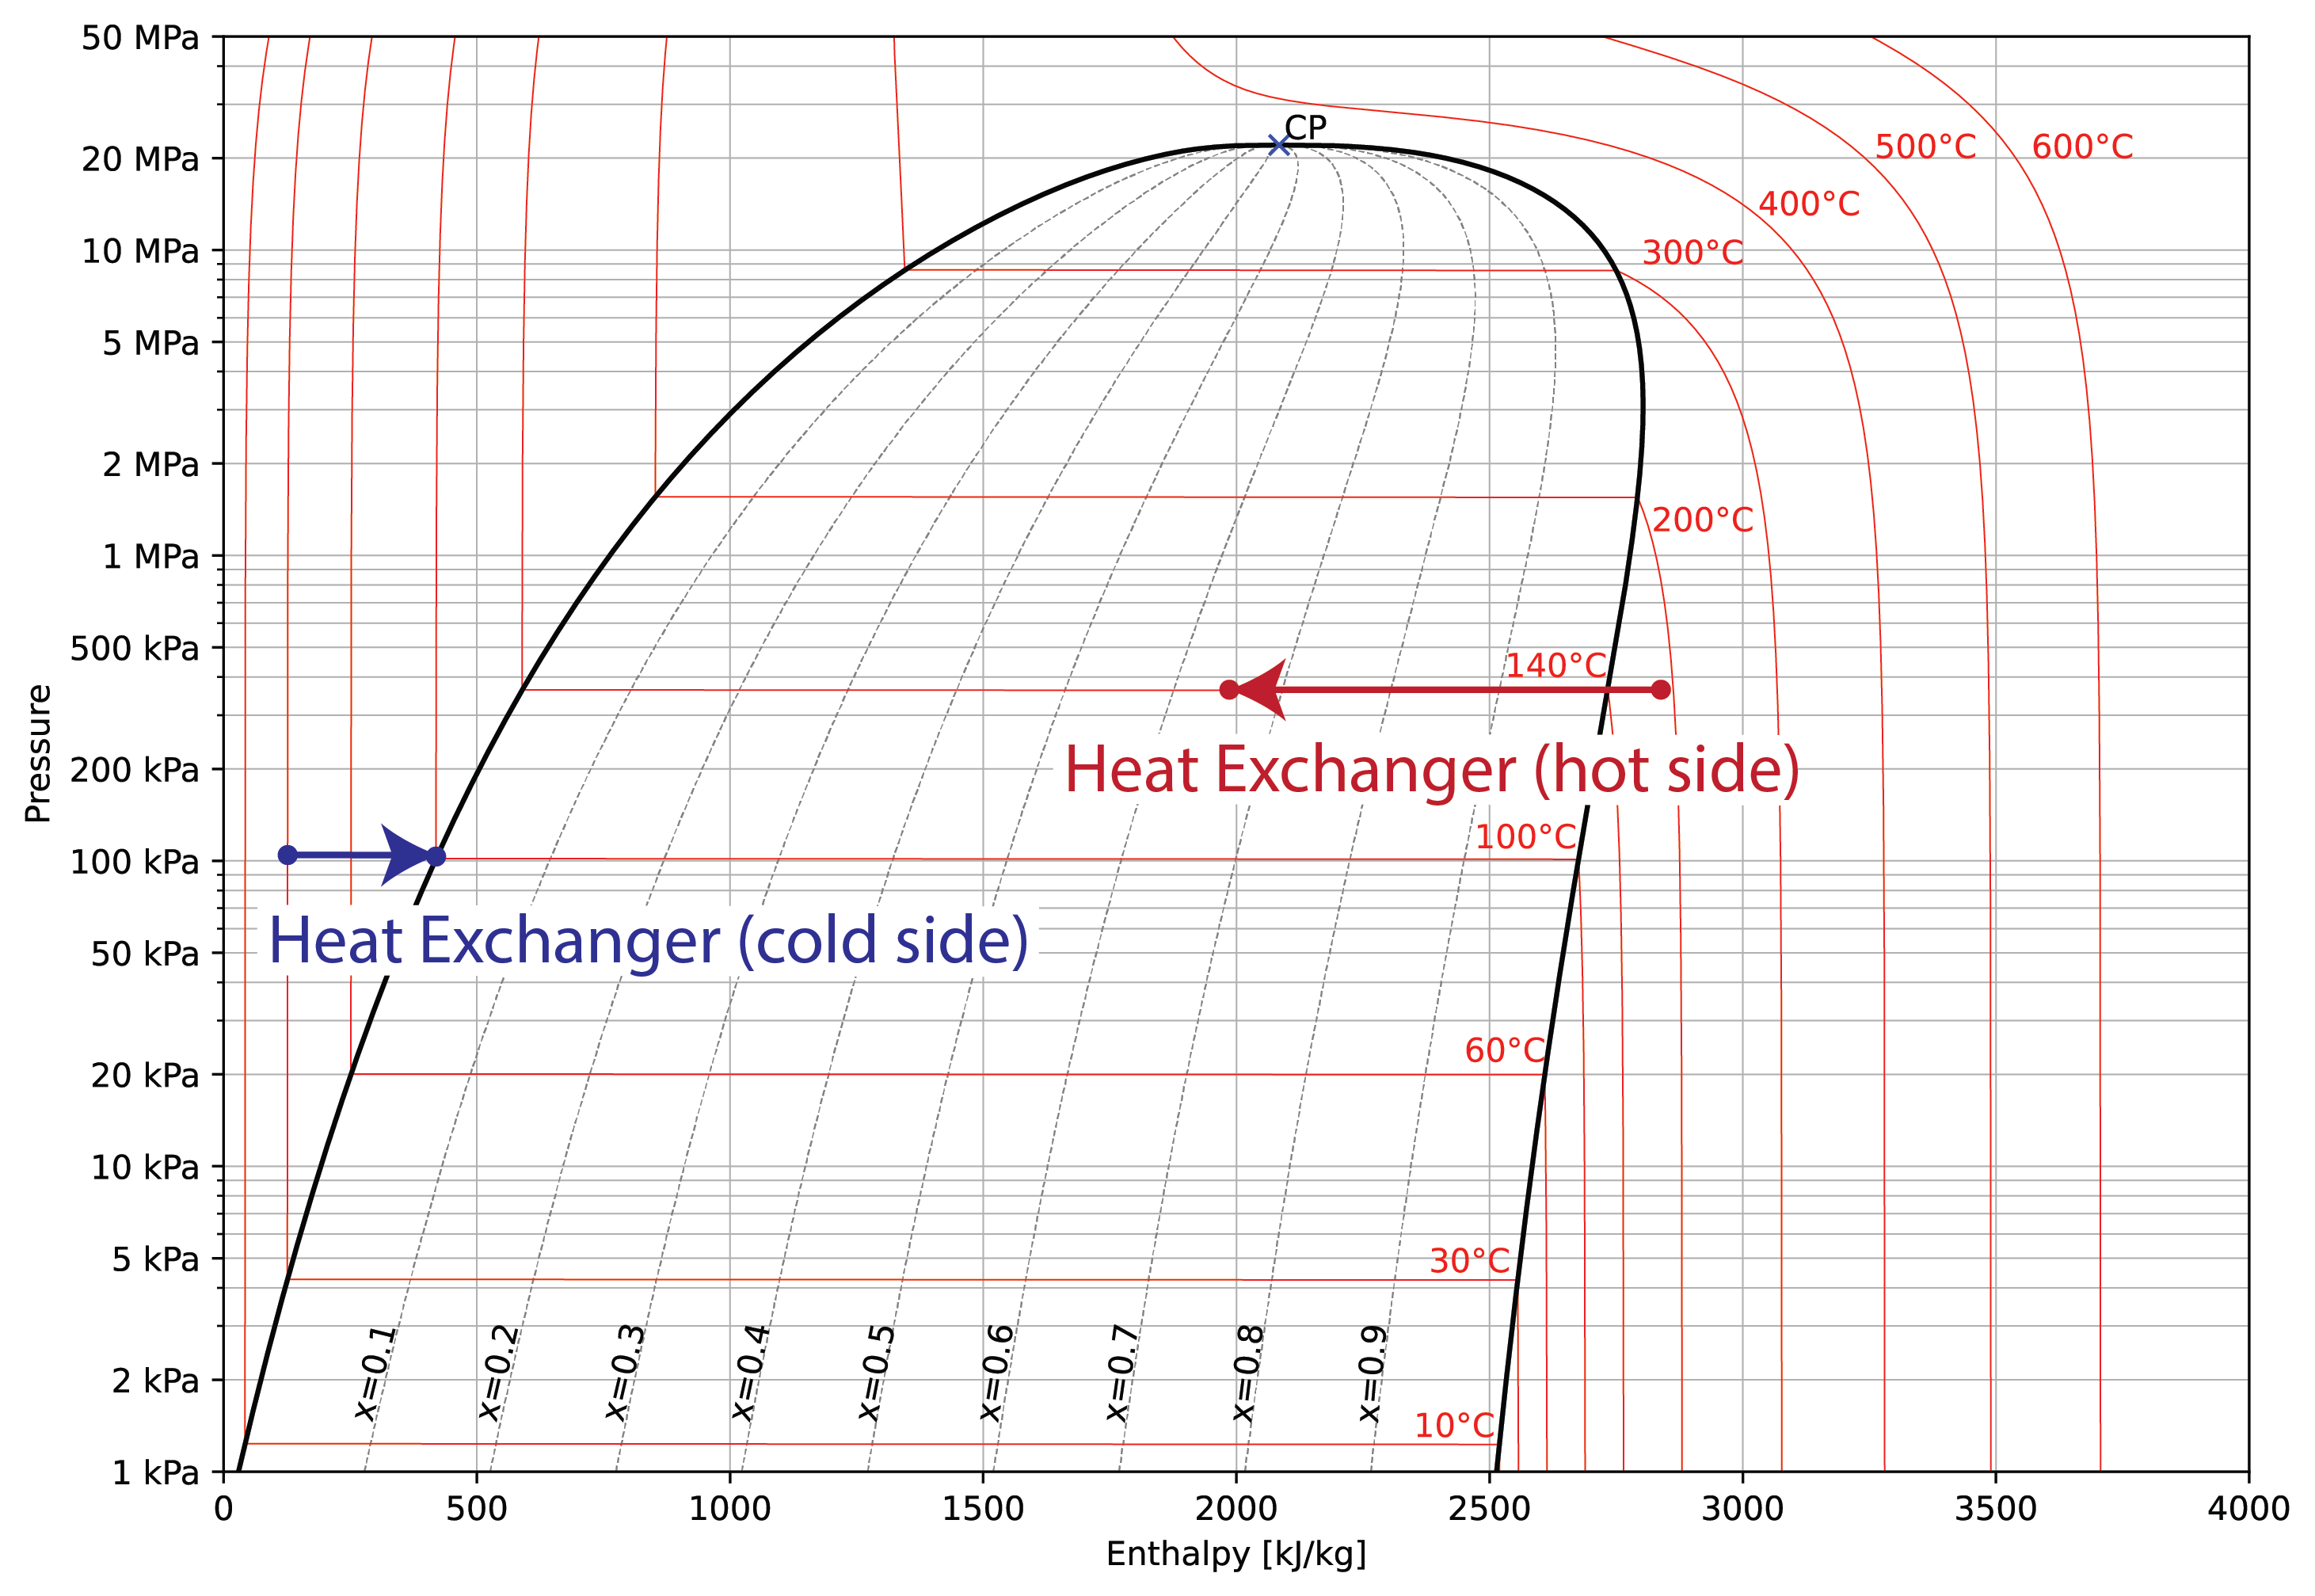
\includegraphics[width=0.75\textwidth]{HeatExchangerph}
\caption{Both hot side and cold side of a heat exchanger plotted on a $p$-$h$ diagram for steam.}
\label{fig:ch4_heatexchangerph}
\end{figure}

The amount of enthalpy gained/lost must satisfy conservation of energy, as written in the Equation \ref{eq:ch4_heatExchanger}.
\begin{equation} \label{eq:ch4_heatExchanger}
  \dot{Q}_{hot} = \dot{m}_{hot} \left(h_{hot, in} - h_{hot, out}\right) = \dot{m}_{cold} \left(h_{cold, out} - h_{cold, in}\right) = \dot{Q}_{cold}
\end{equation}

In reality, boilers, condensers, etc. all qualify as heat exchangers.  The difference is purely in analysis.  We typically consider both the hot and cold flows of heat exchangers, while we are only interested in the heat transfer in boilers, condensers, etc.
% --------------------------------------------------------------------
\subsection{De-aerators}  \label{sec:ch4_deaerators}
De-aerators are used to remove dissolved gases (mostly oxygen) from water in steam power plants, so that they cannot corrode the metal piping or components.  They are therefore an important design consideration for power plants, even though they do not serve a thermodynamic purpose.

In other words, the level of analysis we will perform on these components is minimal.  In Example \ref{ex:ch4FeedwaterHeater}, the de-aerator is combined with the open feedwater heater (a mixer), which is about as in-depth as we get.  Because de-aerators don't significantly change the properties of the fluid, they typically show up as a single state on a $p$-$h$ diagram, rather than a process.

The operation principle behind de-aerators is that the trapped gases have lower solubility (the ability to be dissolved) in hot water than in cold water.  By heating the water up, the trapped gases are forced out of the water, and are then released through a pressure valve.
%
% --------------------------------------------------------------------
\section{Basic Rankine Cycle} \label{sec:RankinePower}
The most basic form of a steam power plant uses the Rankine cycle, shown in Figure \ref{fig:ch4_RankineCycle}.  There are four components in the Rankine cycle: the turbine, boiler, condenser, and pump.

State 1 is traditionally located at the highest temperature/pressure combination, which occurs immediately after the boiler.  The turbine removes work from the system in Process 1-2 (see Section \ref{sec:ch4_turbines}).  State 2 is usually either saturated steam or vapor-liquid mixture with a fairly high quality ($x_2>0.9$).  This steam is piped into a condenser in Process 2-3, which removes enough heat to turn the steam into saturated water (see Section \ref{sec:ch4_condensers}).  Process 3-4 consists of a pump, which significantly increases the pressure of the water by adding work (see Section \ref{sec:ch4_pumps}).  Finally, the water is turned back into steam in the boiler of Process 4-1 (see Section \ref{sec:ch4_boilers}).  This cycle is depicted in Figure \ref{fig:ch4_RankineCycle}.

\begin{figure}[H]
\centering
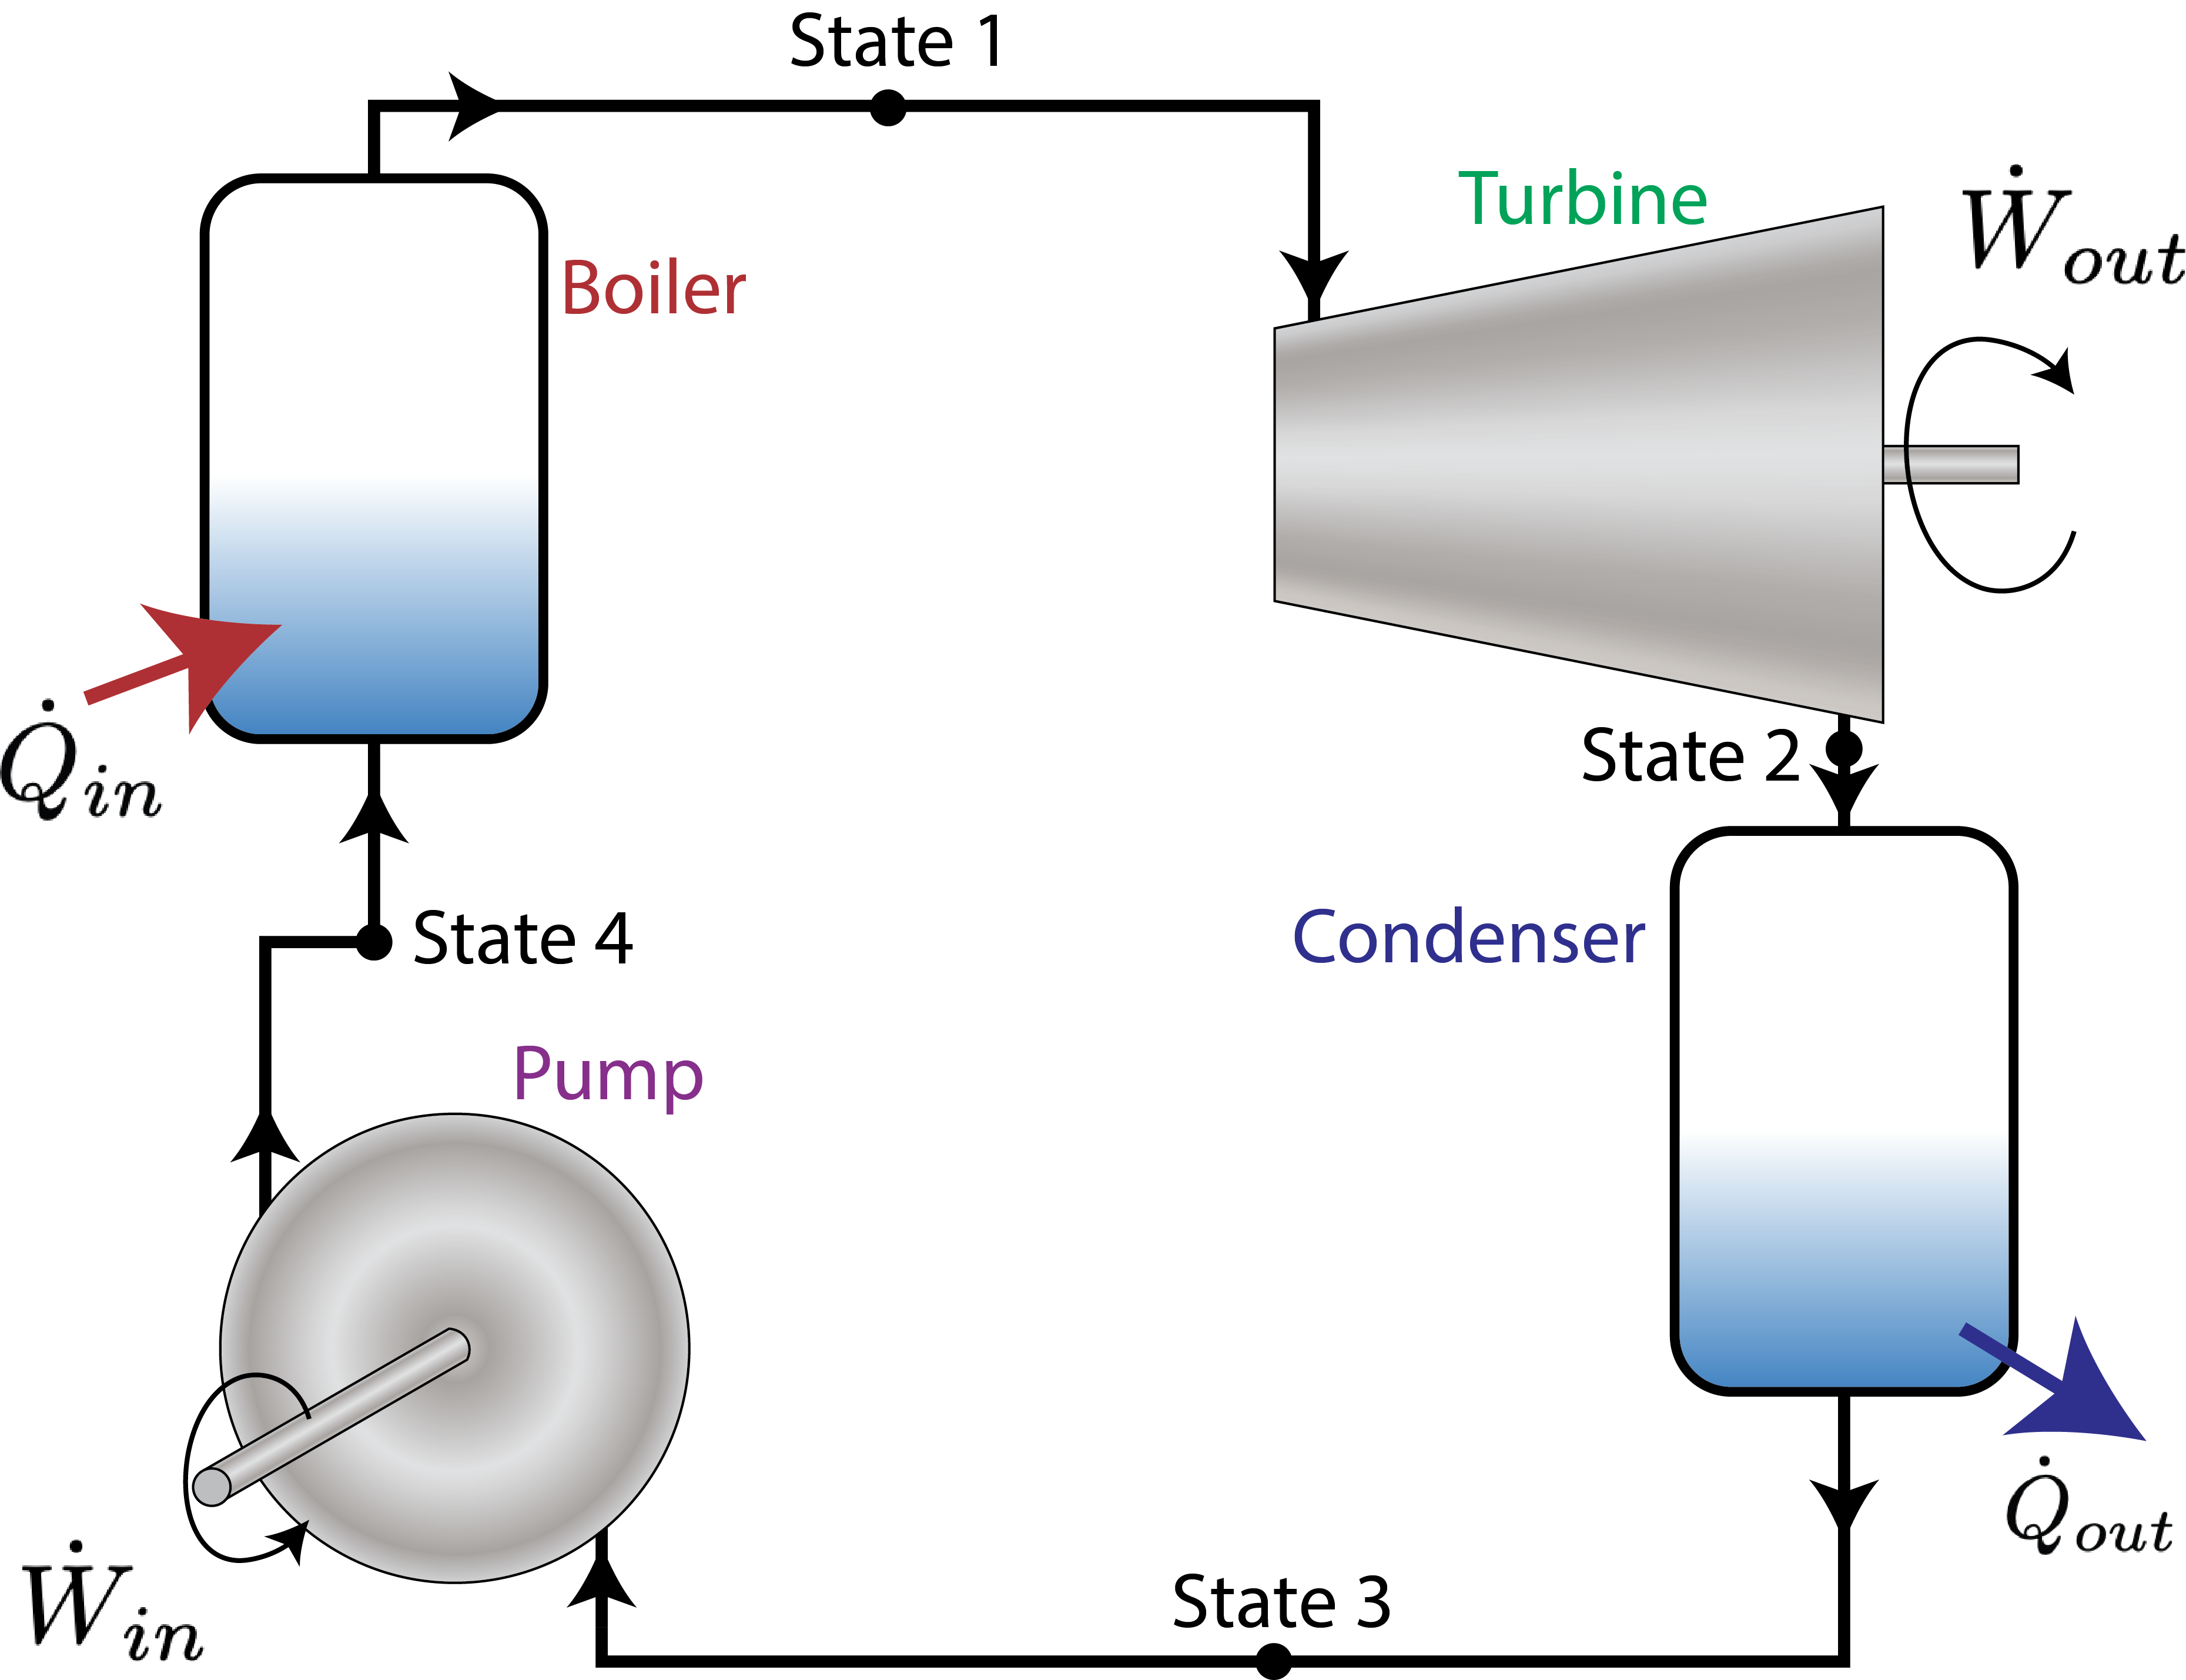
\includegraphics[width=0.75\textwidth]{RankineDiagram}
\caption{Diagram describing the Rankine Cycle for steam power plants.}
\label{fig:ch4_RankineCycle}
\end{figure}

Ideally, for each process, there is an assumption that only work or heat transfer occurs.  In the case of pumps and turbines, this occurs through an adiabatic assumption, which is reasonable given sufficient insulation.  The assumption of no work done occurs in the boiler and condenser because there are typically no moving parts in either of these components, which is a necessary part of adding or extracting energy through work.

For the analysis of this system, we are typically interested in the thermal efficiency, which is defined almost identically to our original definition in Equation \ref{eq:ch3_StirlingEfficiency}.  Of course, we use $\dot{Q}$ instead of $Q$ and $\dot{W}$ instead of $W$:
\begin{equation*} 
  \eta_{th} = \frac{\dot{W}_{net}}{\dot{Q}_{in}} = \frac{w_{net}}{q_{in}}
\end{equation*}

The net work for the Rankine cycle can be defined as $w_{net} = w_{turb}-w_{pump}$.  Often, we neglect the work from the pump, meaning that the net work can be assumed to be equal to the work from the turbine ($w_{net}\approx w_{turb}$).  The heat transfer into the system occurs in the boiler, so $q_{in} = q_{boiler}$.

This gives us an efficiency for the Rankine cycle:
\begin{equation} \label{eq:ch4_RankineEfficiency}
  \eta_{th} = \frac{w_{turb} - w_{pump}}{q_{boiler}} \approx \frac{w_{turb}}{q_{boiler}}
\end{equation}

\begin{figure}[H]
\centering
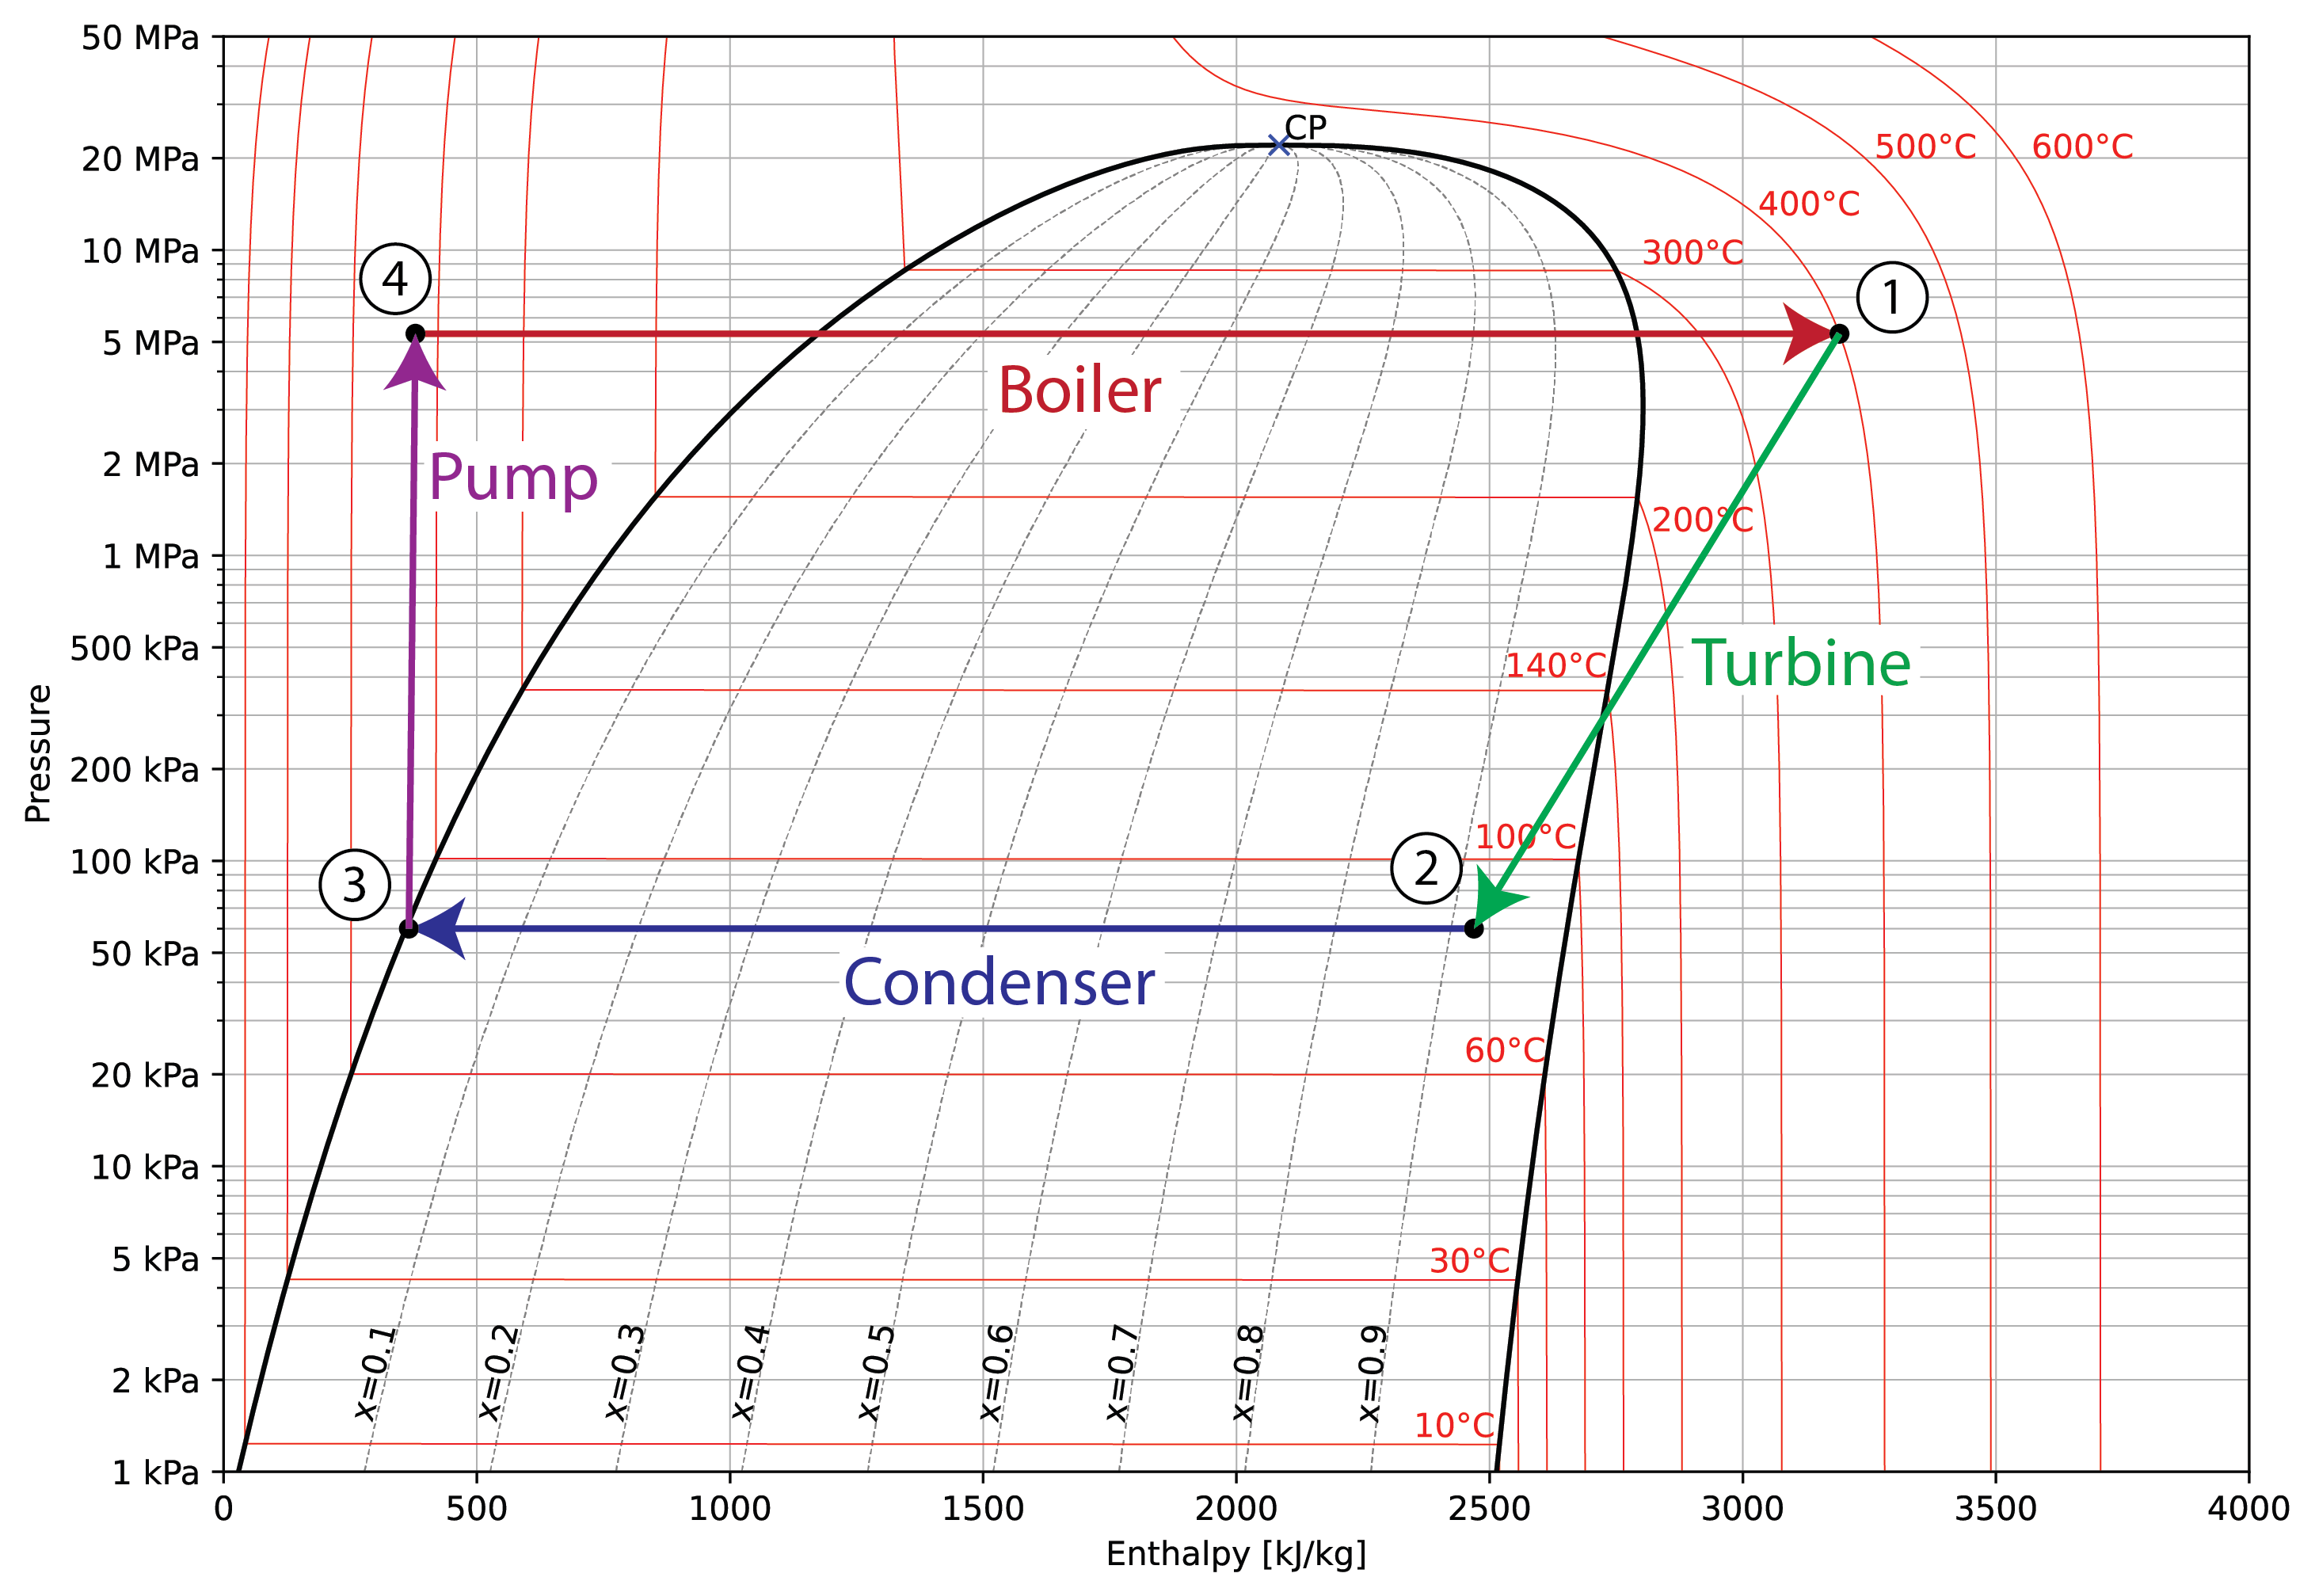
\includegraphics[width=0.9\textwidth]{Rankineph}
\caption{The four processes of the Rankine cycle plotted on a $p$-$h$ diagram for steam.}
\label{fig:ch4_rankineph}
\end{figure}

Because no work occurs in the boiling process, and no heat transfer occurs in the turbine, Equation \ref{eq:controlVolumeEnergyNoKEPE} can be used almost trivially for both the turbine and the boiler:
\begin{align*}
  \dot{m} \Delta h_{1-2} &= \cancelto{0}{\dot{Q}_{1-2}} - \dot{W}_{1-2}  \quad\quad\rightarrow\quad\quad w_{turb} = h_1 - h_2 \\
  \dot{m} \Delta h_{4-1} &= \dot{Q}_{4-1} - \cancelto{0}{\dot{W}_{1-2}}  \quad\quad\rightarrow\quad\quad q_{boil} = h_1 - h_4
\end{align*}
Both of these differences can be seen visually in Figure \ref{fig:ch4_rankineph} as the horizontal distance between states 1 and 2, and states 4 and 1.  Clearly, $h_2 - h_1 < h_1 - h_4$, meaning that more heat is added to the boiler than is extracted from the turbine, giving us an efficiency of less than one, as expected.

We can rewrite the efficiency using only the state enthalpies as follows:
\begin{equation} \label{eq:ch4_RankineEfficiencySimplified}
  \eta_{th} \approx \frac{w_{turb}}{q_{boiler}} = \frac{h_1-h_2}{h_1 - h_4}
\end{equation}

Example \ref{ex:RankineCycle} analyzes a specific Rankine cycle.

%===================================================
\begin{example}[label=ex:RankineCycle]{Rankine Cycle}
  A steam power plant has been designed using the Rankine cycle.  The turbine inlet temperature was chosen to be 500°C, with a pressure at that point of 10 MPa.  After the turbine, the pressure will be 20 kPa, with a quality of 90\%.  The condenser will cool the water to 40°C, and a pump and boiler will complete the cycle.  The flow rate of steam through the power plant will be 8 kg/s.

  Using this information, do the following:
  \begin{enumerate}[a)]
  \item draw each of the states and processes on the $p$-$h$ diagram for water
  \item find the power of the turbine and feedwater pump
  \item find the heat transfer rates of the boiler and condenser
  \item calculate the thermal efficiency of the system
  \end{enumerate}

  \subsection*{Solution Methodology}
  To start, we will create a table with the given information of each of the states, looking at Figure \ref{fig:ch4_RankineCycle} to define each state.  For instance, the ``turbine inlet'' refers to State 1, as it is the state immediately before the turbine.

  After we find the relevant information for all of the states, we will create a $p$-$h$ diagram for part a), then use that diagram to find the power and heat transfer rates for each of the components.  The thermal efficiency will naturally follow once we know the specific work and heat transfer for each process.

  \subsubsection{State 1 and 2 Properties}
  It is possible to fill in the remaining information for States 1 and 2, as both have two properties defined.  In this case, $h_1$ can be read directly from Appendix \ref{app:steam_super}, and $h_2$ can be found using Appendix \ref{app:steam_satP} and Equation \ref{eq:quality}:
  \begin{equation*}
    h_2 = x h_g + (1-x) h_f = 0.9 \left(2608.9\  \frac{\rm kJ}{\rm kg}\right) + 0.1 \left(251.42\ \frac{\rm kJ}{\rm kg}\right) = 2373.2\ \frac{\rm kJ}{\rm kg}
  \end{equation*}

  \begin{table}[H]
    \centering
    \def\arraystretch{1.5}
    %\caption{Tabular Representation of Energy Equation for Stirling Cycle}
    %\label{tab:ch3_stirling}
    \begin{tabular}{r|cccc}
      & State 1 & State 2 & State 3 & State 4 \\ \hline
      Pressure    & 10 MPa  & 20 kPa  &         &         \\
      Temperature & 500°C   & ${\color{Red} 60.06{\rm °C}}$   &  40°C   &     \\
      Enthalpy    & ${\color{Red} 3375.1 \frac{\rm kJ}{\rm kg}}$        & ${\color{Red} 2373.2 \frac{\rm kJ}{\rm kg}}$       &         &         \\
      Quality     & -       & 0.9     &         & 
    \end{tabular}
    \def\arraystretch{1.0}
  \end{table}
  
% --------------------------------------------------------------------
\subsubsection*{State 3 Properties}

To find the properties of State 3, we refer to Section \ref{sec:ch4_condensers}.  The key assumption for us here is that the pressure will remain constant across the condenser.  This gives us a pressure of $p_3 = 20\ \rm kPa$, which allows us to find the rest of the properties.

Unfortunately, we run into a small hitch in this process, which is that the most relevant chart, Appendix \ref{app:water_compressed} does not have data anywhere near 20 kPa.  We therefore use the assumption that the enthalpy will be very near the enthalpy of saturated water at 40°C.  This gives us an enthalpy of $h_3 = 167.53\ \frac{\rm kJ}{\rm kg}$.

Alternatively, we can use CoolProp to determine the properties, including the effect of the slightly higher pressure.  After our normal setup, we use the following command (converting to Pascals and Kelvin as needed):
\begin{Verbatim}[commandchars=\\\{\}]
print( CP.PropsSI(\textcolor{purple}{'H'}, \textcolor{purple}{'P'}, \textcolor{JungleGreen}{20e3}, \textcolor{purple}{'T'}, \textcolor{JungleGreen}{40} + \textcolor{JungleGreen}{273.15}, \textcolor{purple}{'water'}) )
\end{Verbatim}
This command returns a value of 167544.2, which, according to Table \ref{tab:ch2_CoolProp}, has units of J/kg.  Converting to kJ/kg, we get that $h_3 = 167.54\ \frac{\rm kJ}{\rm kg}$, which is functionally equivalent to the value from the tables.

% --------------------------------------------------------------------
\subsubsection*{State 4 Properties}

To find the properties of State 4, we refer to Section \ref{sec:ch4_pumps} and Section \ref{sec:ch4_boilers}.  The assumption that boilers operate under constant pressure allows us to set $p_4 = p_1 = 10\ \rm MPa$, while the assumption that pumps operate under constant temperature allows us to set $T_4 = T_3 = 40\rm °C$.  The enthalpy after the pump can therefore be read directly from Appendix \ref{app:water_compressed} as $h_4 = 176.36\ \frac{\rm kJ}{\rm kg}$.

Alternatively, if the tables are not so clean, we can follow the methodology from Equation \ref{eq:ch4_pumpEnthalpy}:
\begin{align*}
  \Delta h &= v\Delta p \quad \rightarrow \quad h_4 - h_3 = v(p_4 - p_3) \\
  h_4 &= 167.54\ \frac{\rm kJ}{\rm kg} + 0.001\ \frac{\rm m^3}{\rm kg} \left(10,000 {\rm kPa} - 20 kPa \right) = 177.52\ \frac{\rm kJ}{\rm kg} 
\end{align*}

While this is not perfect, it is a fair approximation.

This allows us to complete our property table.
  \begin{table}[H]
    \centering
    \def\arraystretch{1.5}
    %\caption{Tabular Representation of Energy Equation for Stirling Cycle}
    %\label{tab:ch3_stirling}
    \begin{tabular}{r|cccc}
      & State 1 & State 2 & State 3 & State 4 \\ \hline
      Pressure    & 10 MPa  & 20 kPa  &  {\color{Red} 20 kPa} &  {\color{Red} 10 MPa}       \\
      Temperature & 500°C   & 60.06°C &  40°C   & ${\color{Red} 40{\rm °C}}$  \\
      Enthalpy    & 3375.1 $\frac{\rm kJ}{\rm kg}$  & 2373.2 $\frac{\rm kJ}{\rm kg}$  &  $\color{Red} 167.54 \frac{\rm kJ}{\rm kg}$  & $\color{Red}176.36 \frac{\rm kJ}{\rm kg}$     \\
      Quality     & -       & 0.9     &   -      &  -
    \end{tabular}
    \def\arraystretch{1.0}
  \end{table}
  % --------------------------------------------------------------------
  \subsubsection*{$p$-$h$ Diagram}
  With the pressure and enthalpy defined for each state, we can now complete our $p$-$h$ diagram. $\Delta h$ for each process can be clearly seen by looking at the horizontal distance between the two states.  Thus we see that the heat added in the boiler is the largest contribution, while the work done by the pump is negligible.

  \begin{figure}[H]
    \centering
    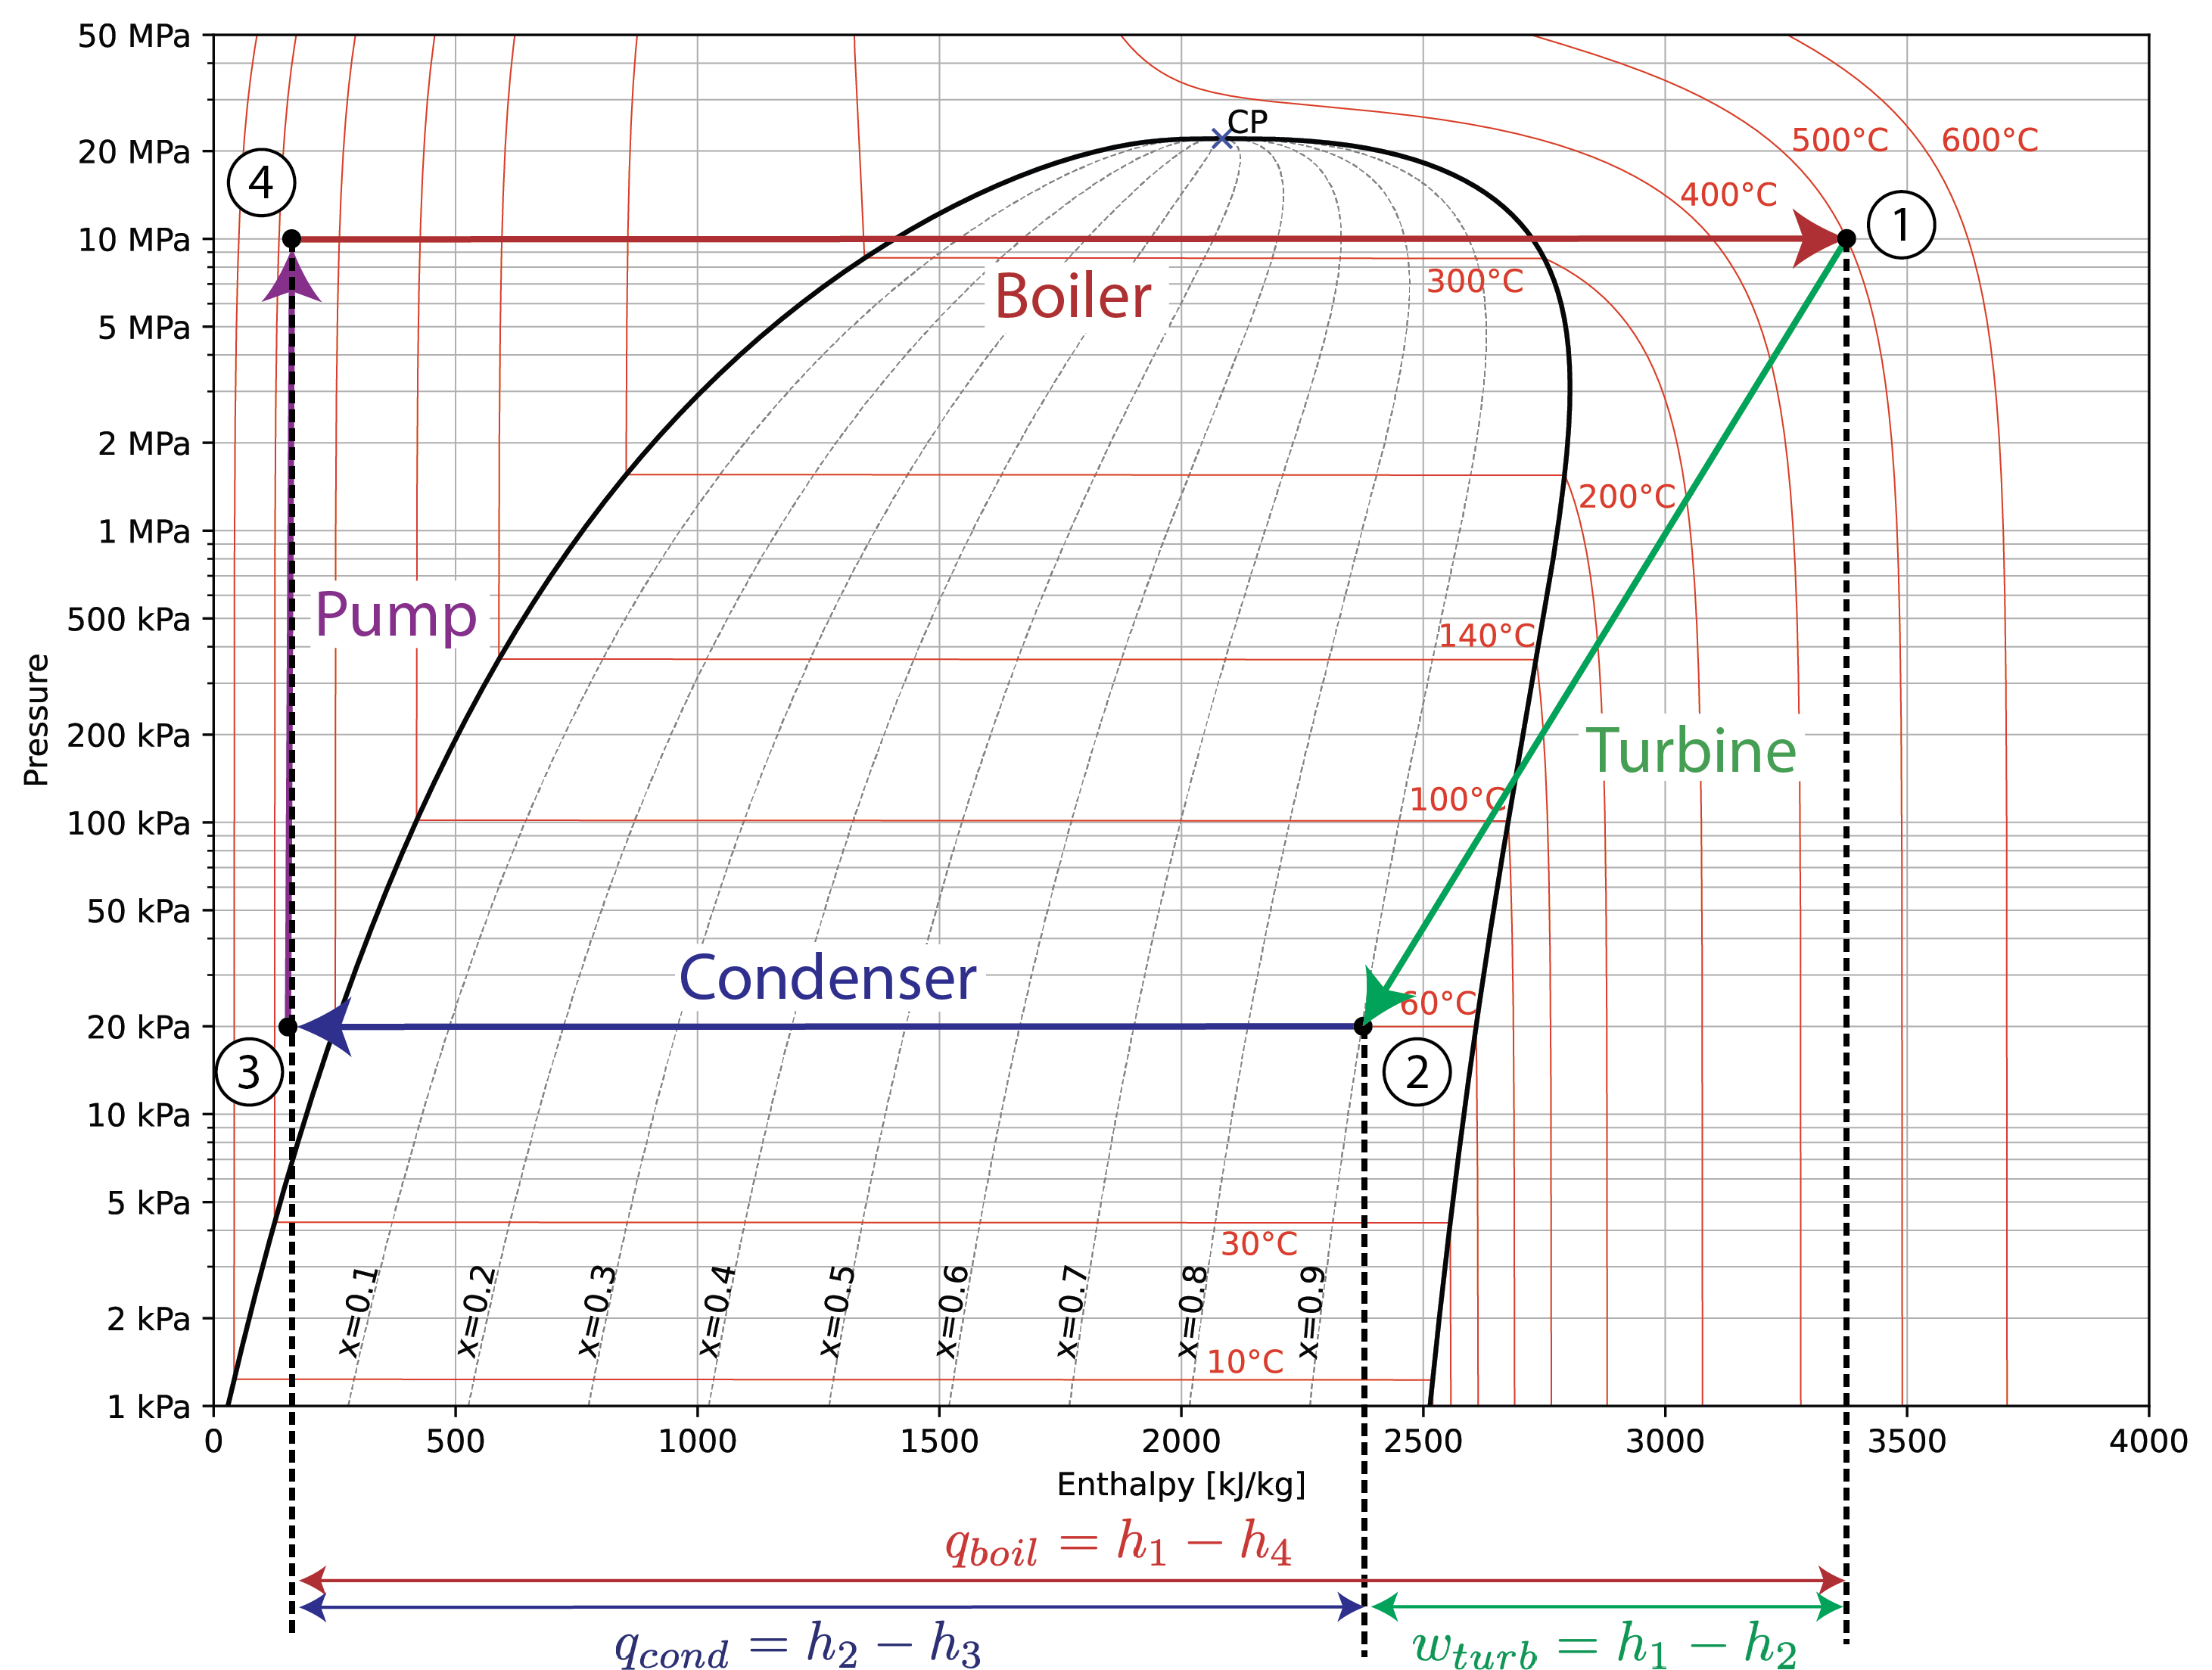
\includegraphics[width=0.9\textwidth]{RankineExample}
    %\caption{The four processes of the Rankine cycle plotted on a $p$-$h$ diagram for steam.}
  \end{figure}

  Additionally, plotting our cycle on the $p$-$h$ diagram allows us to double check our enthalpies at each state.  We can see that $h_1$ is about 3400 kJ/kg, $h_2$ is approximately 2300 kJ/kg, and both $h_3$ and $h_4$ are between 100 and 200 kJ/kg.  These match our calculated values and let us know we are on the right track.
  \subsubsection*{Process Work and Heat Transfer}

  With our enthalpies calculated, it is straightforward to calculate the work and heat transfer for each process.  Both pumps and turbines are typically assumed to be adiabatic, meaning that we can say $w_{turb} = h_1 - h_2 = 1002\ \rm\frac{kJ}{kg}$ and $w_{pump} = h_4 - h_3 = 11\ \rm\frac{kJ}{kg}$.  Both of these are typically defined to be positive, even though the turbine results in positive work, while the pump is associated with negative work.

  Likewise, no work occurs in the condenser or boiler, meaning that $q_{boil} = h_1 - h_4 =  3199\ \rm\frac{kJ}{kg}$ and $q_{cond} = h_2 - h_3 = 2206\ \rm\frac{kJ}{kg}$.  Again, both heat transfers are defined to be positive, even though the condenser removes heat from the system.

  The $w$ and $q$ values are all mass-specific.  In order to find the actual values for the power plant, we need to multiply by the mass flow rate, $\dot{m}$.

  \begin{align*}
    \dot{W}_{turb} &= \dot{m}\ w_{turb} = 8\ \frac{\rm kg}{\rm s} \cdot 1002\ \frac{\rm kJ}{\rm kg} = 8016\ {\rm kW} = 8.0\ {\rm MW} \\
    \dot{W}_{pump} &= \dot{m}\ w_{pump} = 8\ \frac{\rm kg}{\rm s} \cdot 11\ \frac{\rm kJ}{\rm kg} = 88\ {\rm kW} = 0.088\ {\rm MW} \\
    \dot{Q}_{boil} &= \dot{m}\ q_{boil} = 8\ \frac{\rm kg}{\rm s} \cdot 3199\ \frac{\rm kJ}{\rm kg} = 25,592\ {\rm kW} = 25.6\ {\rm MW} \\
    \dot{Q}_{cond} &= \dot{m}\ q_{cond} = 8\ \frac{\rm kg}{\rm s} \cdot 2206\ \frac{\rm kJ}{\rm kg} = 17,648\ {\rm kW} = 17.6\ {\rm MW} 
  \end{align*}

  \subsubsection*{Thermal Efficiency}

  Finally, we can calculate the efficiency of the process.  The net work is simply $w_{net} = w_{turb} - w_{pump}$, and the heat transfer into the system occurs solely in the boiler: $q_{in} = q_{boil}$.
  \begin{equation*}
    \eta_{th} = \frac{w_{net}}{q_{in}} = \frac{w_{turb}-w_{pump}}{q_{boil}}=\frac{1002\ \rm\frac{kJ}{kg} - 11\ \rm\frac{kJ}{kg}}{3199\ \rm\frac{kJ}{kg}} = 0.310
  \end{equation*}

  Thus, the thermal efficiency of the system above is 31.0\%.  Neglecting the work from the pump results in an efficiency of 31.3\%.  Clearly it is more accurate to include the work spent on running the pump, but there is a question whether the increased accuracy justifies the extra work in this case.  Quite frankly, there are other losses and assumptions that are substantially more significant, and unless we address those, neglecting the pump is perfectly reasonable.
  
\end{example}
%===================================================

% --------------------------------------------------------------------
\section{Modifications to the Rankine Cycle}
% --------------------------------------------------------------------
The Rankine cycle is a good baseline to understand steam power plants.  However, most power plants require additional components to create an accurate model.  Most commonly, there is not a single turbine, but several, typically labeled as ``high pressure'' and ``low pressure'' turbines.  Functionally, there is no difference between having a single turbine or multiple turbines, except that it provides an opportunity to do something with the steam in between.

Section \ref{sec:ch4_reheat} looks at the possibility of {\bf re-heating} the steam in between the high pressure and low pressure turbines.  The power plant in Section \ref{sec:ch4_regen} extracts some of the steam between the turbines and mixes it with cold water before the pump in a process called {\bf regeneration}.

Other modifications to the cycle include getting heat from more than one source in a {\bf hybrid} plant, or using excess heat for other purposes (known as {\bf cogeneration}).  These modifications are looked at in the homework problems for this chapter.

\subsection{Rankine Cycle with Reheat} \label{sec:ch4_reheat}
% --------------------------------------------------------------------
The Rankine Cycle with reheat includes a separation between the low pressure and high pressure turbines, which allows for steam to be sent back to the boiler.  The steam is reheated either to around the same temperature as State 1, and is then sent to the low pressure turbine.  As before, the boiler does not change the pressure of the steam in the reheat process.

\begin{example}[label=ex:ch4_supercrit]{Nuclear Power Plant with Reheat}
  Modern nuclear power plants typically use pressurized water to transport heat outside of the core.  Because of this, they tend to be rather limited in temperature (one of the benefits of molten salt nuclear reactors is the ability of the salt to transport heat at much higher temperatures).

  For this example, we are looking at a steam turbine loosely based off of \href{https://www.ge.com/steam-power/products/steam-turbines}{General Electric's  steam turbines for nuclear applications}.  The high-pressure turbine inlet pressure and temperature will be 7.5 MPa and 300°C, respectively.  After the high-pressure turbine, the steam goes back to the boiler and is again heated to 300°C.  This lower pressure steam is sent to the low-pressure turbine, after which it finally goes through the rest of the cycle.  The diagram for this is shown in the figure below.

  \begin{center}
    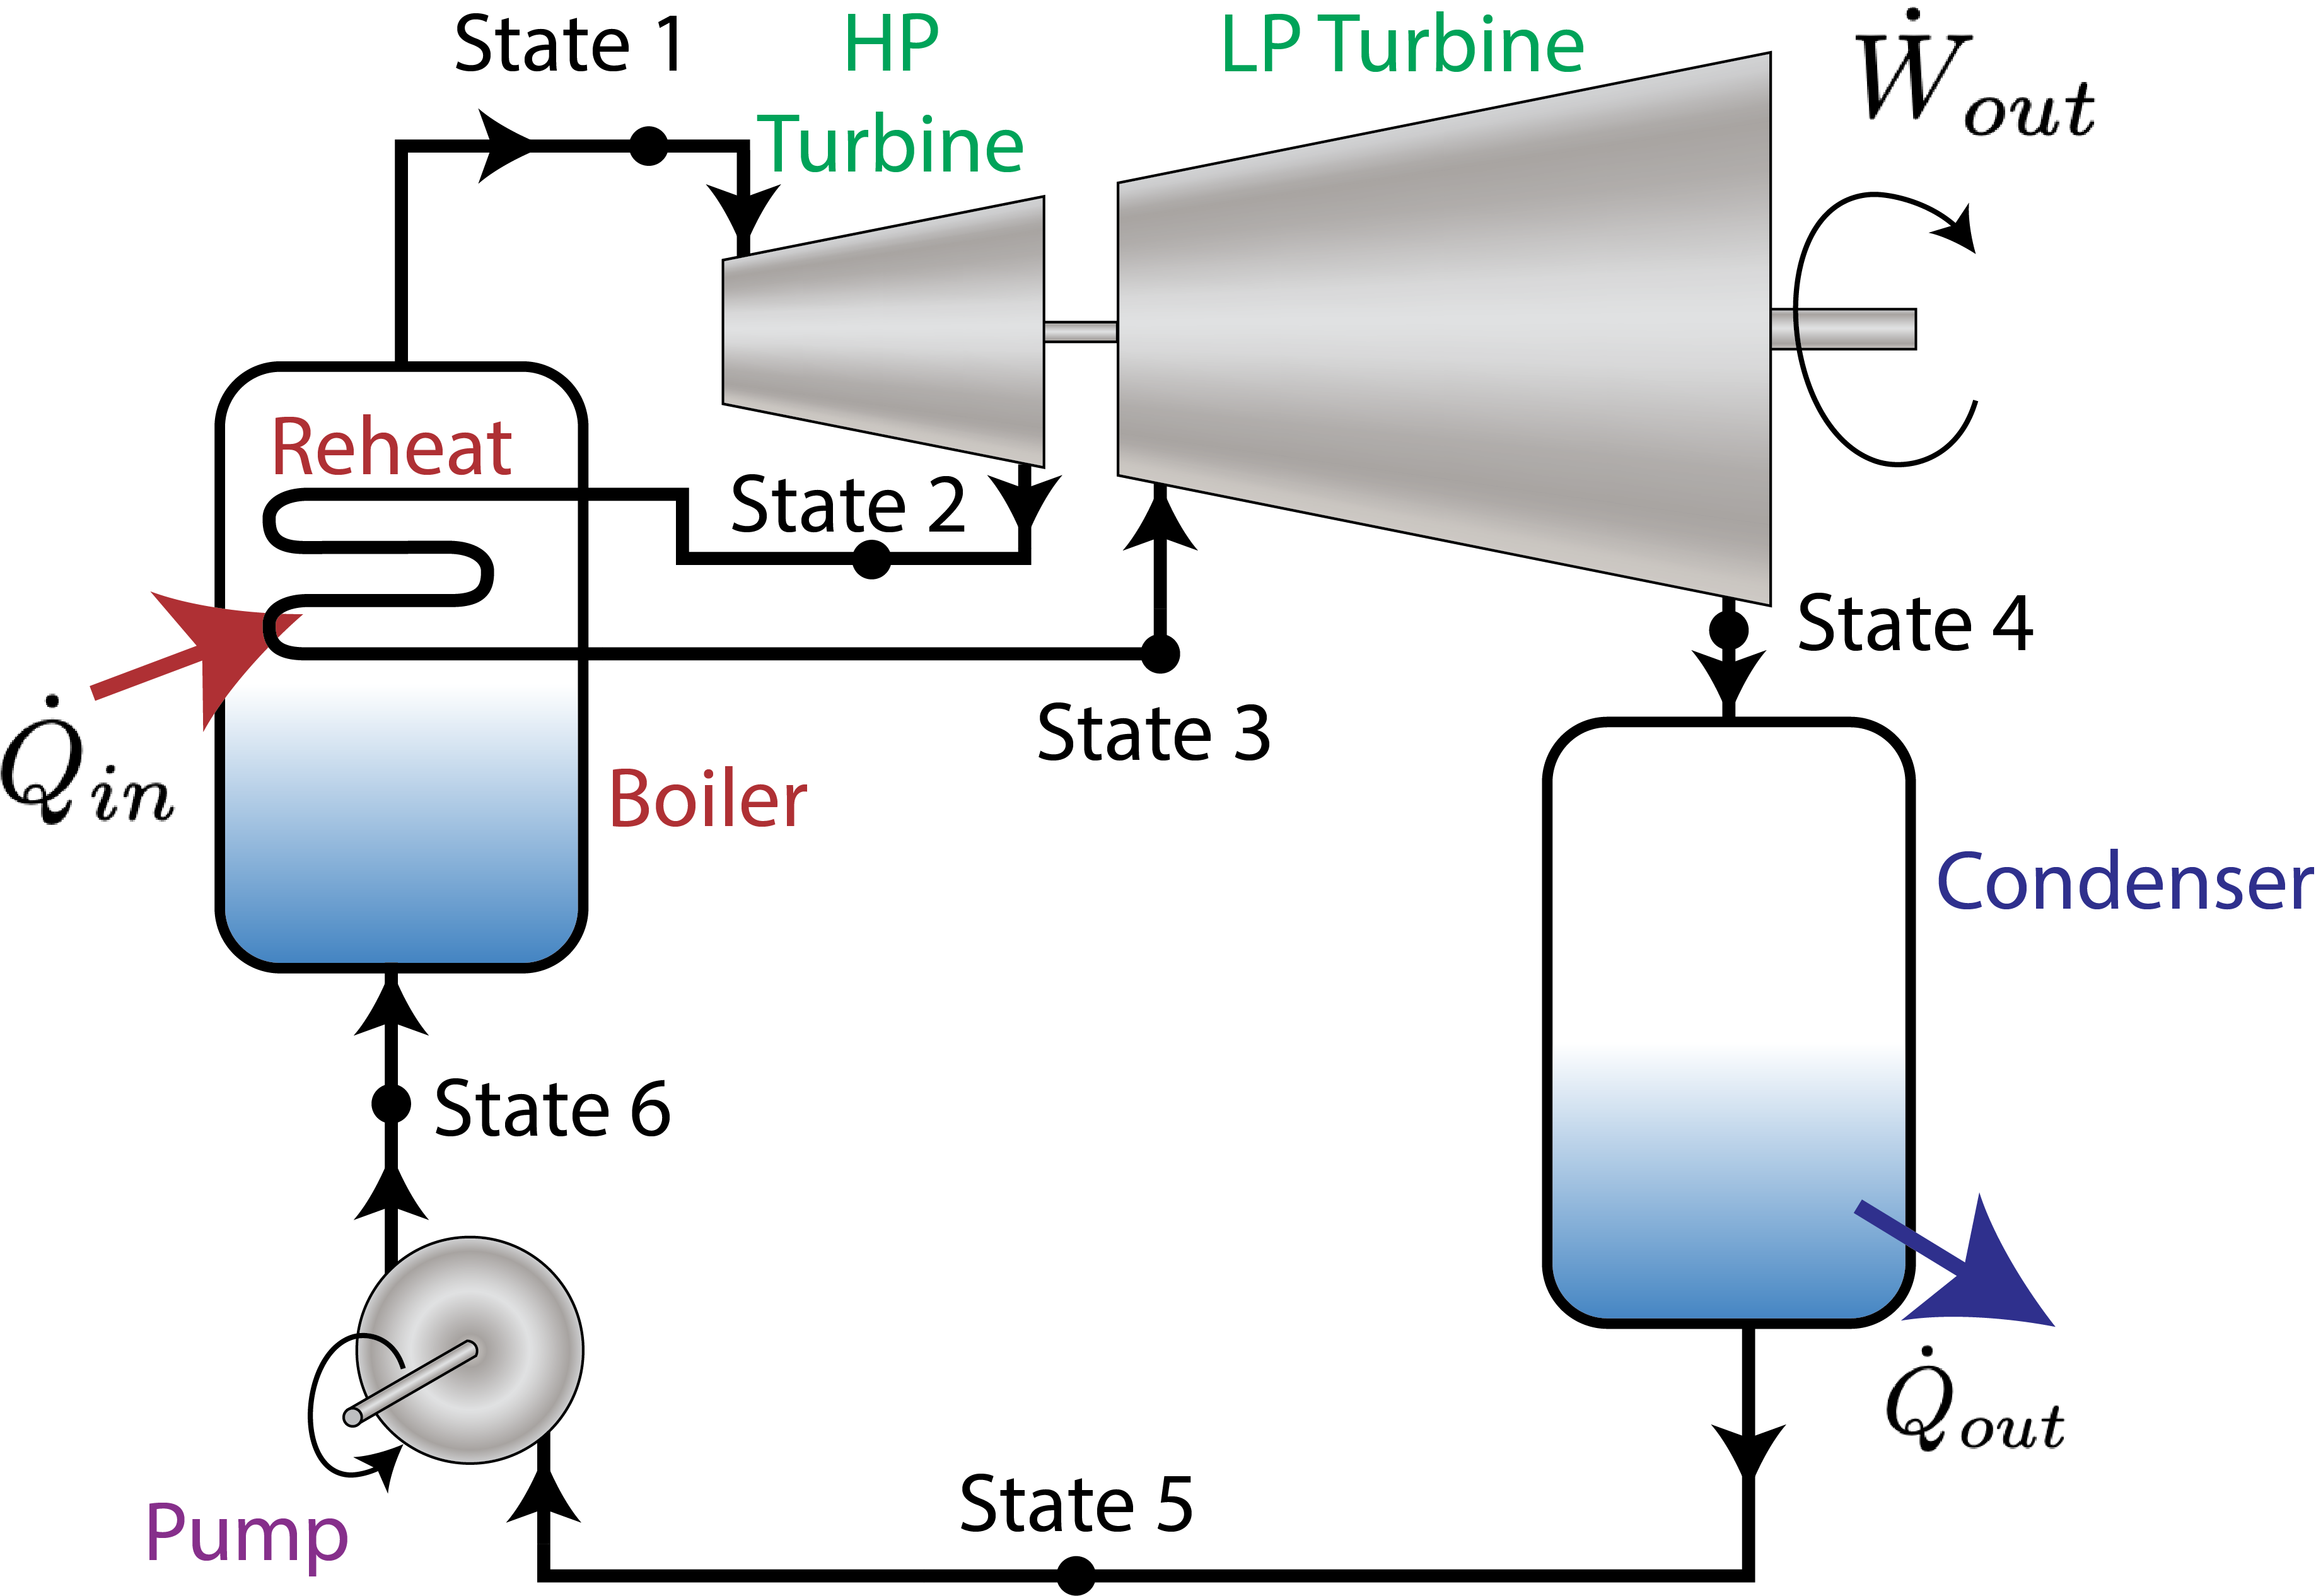
\includegraphics[width=0.75\textwidth]{RankineWithReheat}
    %\captionof{figure}{}
    %\label{fig:ch2_example1}
  \end{center}
  \subsection*{Solution Methodology}
  In this example, we will first build the $p$-$h$ diagram, then fill out the table of properties afterwards.  We know that State 1 is at 7.5 MPa and 300°C from GE's specifications.  We will choose State 2 to be 2.5 MPa, with a quality of 0.9.  State 3 will have the same pressure as State 2, but with a temperature of 300°C again.  Again, we choose a quality of 0.9 for State 4, this time with a pressure of 100 kPa.  The condenser will cool the water at State 5 to 60°C, still with a pressure of 100 kPa.  Finally, the pump will maintain a temperature of 60°C for State 6, but return the pressure to 7.5 MPa.

  With this information, we will be able to perform the following:

  \begin{enumerate}[a)]
  \item Plot the cycle on a $p$-$h$ diagram, using temperature, pressure, and quality lines to find the states.
  \item Complete a table of properties for each state.
  \item Determine the work extracted from the turbines per kg of steam.
  \item Determine the total energy needed from heat transfer in the boiler and reheat processes per kg of steam.
  \item Find the amount of heat rejected by the condenser per kg of steam.
  \item Determine the amount of work required to run the pump per kg of steam.  Compare values from CoolProp and using the incompressible assumption.
  \item Find the mass flow rate of steam needed to generate 450 MW of power in the turbines.
  \item Find the efficiency of the power plant and the total heat transfer rate required from the nuclear reactor.
  \end{enumerate}

  \subsubsection*{$p$-$h$ Diagram}
  
  \begin{center}
    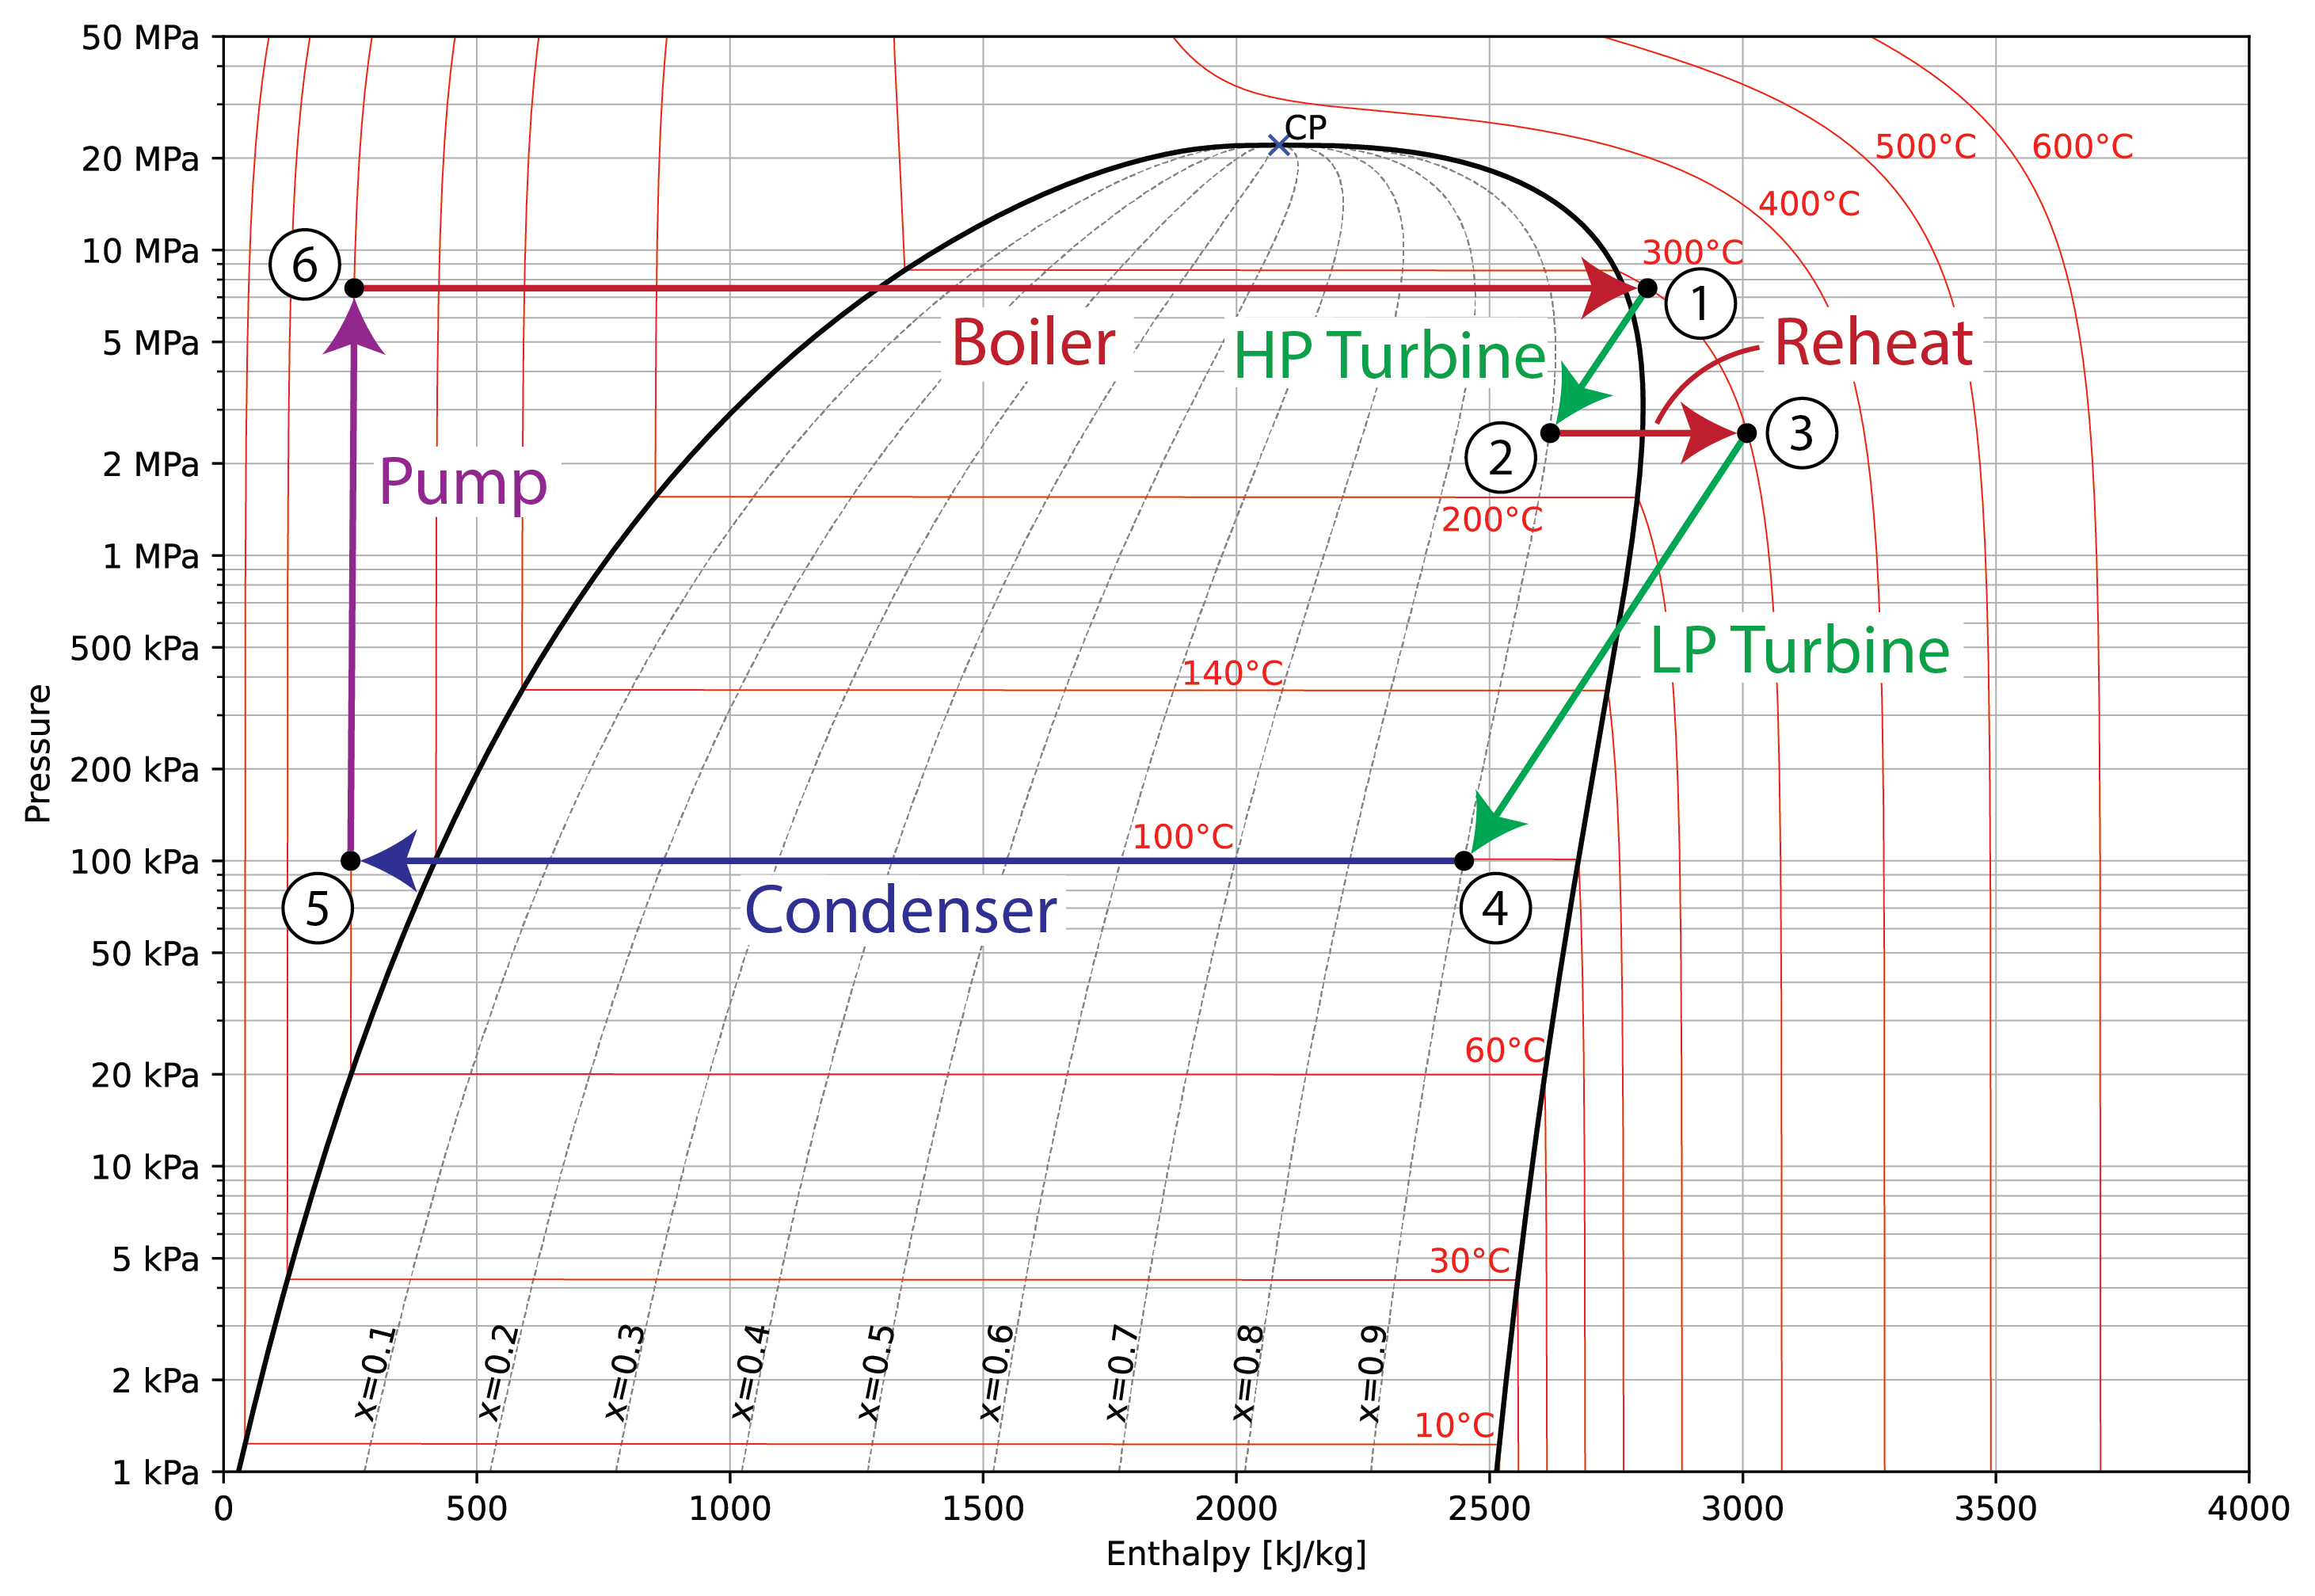
\includegraphics[width=0.9\textwidth]{RankineReheatph}
    %\captionof{figure}{}
    %\label{fig:ch2_example1}
  \end{center}

  The beauty of the $p$-$h$ diagram is that we can get a picture of the cycle without ever looking at tables.
  \begin{itemize}
  \item The relatively low temperature of State 1 means that the HP Turbine cannot extract much work without bringing the steam below a quality of 0.9.
  \item The heat absorbed in the reheat process is substantially less than the original boiling.
  \item The LP turbine is able to extract much more heat than the HP turbine, in conjunction with a much larger pressure drop.
  \end{itemize}

  \subsubsection*{Property Table}
  The properties of States 1, 3, and 6 are simple table look-ups (with interpolation required for States 1 and 6).  States 2 and 4 require use of Equation \ref{eq:quality}, and State 5 can either be assumed to be equivalent to saturated water at 60°C or evaluated using CoolProp.  The table below is populated purely from CoolProp, so small differences may be present compared to interpolation of tables.  Quantities in black are taken from the problem statement, and quantities in red are calculated.
  \begin{table}[H]
    \centering
    \def\arraystretch{1.5}
    %\caption{Tabular Representation of Energy Equation for Stirling Cycle}
    %\label{tab:ch3_stirling}
    \begin{tabular}{r|cccc}
      State & Pressure & Temperature & Enthalpy & Quality \\ \hline
      1 & 7.5 MPa & 300°C & {\color{Red} 2814.4 $\frac{\rm kJ}{\rm kg}$} & - \\
      2 & 2.5 MPa & {\color{Red} 224°C} & {\color{Red} 2617.9 $\frac{\rm kJ}{\rm kg}$} & 0.9 \\
      3 & 2.5 MPa & 300°C & {\color{Red} 3009.6 $\frac{\rm kJ}{\rm kg}$} & - \\
      4 & 100 kPa & {\color{Red} 100°C} & {\color{Red} 2449.2 $\frac{\rm kJ}{\rm kg}$} & 0.9 \\
      5 & 100 kPa & 60°C & {\color{Red} 251.3 $\frac{\rm kJ}{\rm kg}$} & - \\
      6 & 7.5 MPa & 60°C & {\color{Red} 257.5 $\frac{\rm kJ}{\rm kg}$} & - 
    \end{tabular}
    \def\arraystretch{1.0}
  \end{table}
  \subsubsection*{Turbine/Pump Work, Boiler/Reheat/Condenser Heat Transfer}
  The specific work obtained from each turbine is exactly the difference in enthalpy between the states, due to the assumption of adiabatic turbines.  Thus:
  \begin{align*}
    w_{HPT} &= h_1 - h_2 = 2814.4\ \frac{\rm kJ}{\rm kg} - 2617.9\ \frac{\rm kJ}{\rm kg} = 196.5\ \frac{\rm kJ}{\rm kg} \\
    w_{LPT} &= h_3 - h_4 = 3009.6\ \frac{\rm kJ}{\rm kg} - 2449.2\ \frac{\rm kJ}{\rm kg} = 560.4\ \frac{\rm kJ}{\rm kg} \\
    w_{turb} &= w_{HPT} + w_{LPT} = \redbox{756.9\ \frac{\rm kJ}{\rm kg}}
  \end{align*}

  The pump can be found the same way:
  \begin{equation*}
    w_{pump} = h_6 - h_5 = 257.5\ \frac{\rm kJ}{\rm kg} - 251.3\ \frac{\rm kJ}{\rm kg} = \redbox{6.2\ \frac{\rm kJ}{\rm kg}}
  \end{equation*}

  Alternatively, we can use Equation \ref{eq:ch4_pumpEnthalpy}:
  \begin{equation*}
    w_{pump} = 0.001\ \frac{\rm m^3}{\rm kg} \left(7500\ {\rm kPa} - 100\ {\rm kPa}\right) = \redbox{7.4\ \frac{\rm kJ}{\rm kg}}
  \end{equation*}

  We'll use the CoolProp value of 6.2 $\frac{\rm kJ}{\rm kg}$.
  
  Similarly, there is no work that occurs in the boiler or reheat cycle, meaning we can again use the difference in enthalpy:
  \begin{align*}
    q_{boiler} &= h_1 - h_6 = 2814.4\ \frac{\rm kJ}{\rm kg} - 257.5\ \frac{\rm kJ}{\rm kg} = 2556.9\ \frac{\rm kJ}{\rm kg} \\
    q_{reheat} &= h_3 - h_2 = 3009.6\ \frac{\rm kJ}{\rm kg} - 2617.9\ \frac{\rm kJ}{\rm kg} = 391.7\ \frac{\rm kJ}{\rm kg} \\
    q_{in} &= w_{boiler} + w_{reheat} = \redbox{2948.6\ \frac{\rm kJ}{\rm kg}}
  \end{align*}

  Finally, we can calculate the heat transfer in the condenser, again assuming no work occurs:
   \begin{equation*}
    q_{cond} = h_4 - h_5 = 2449.2\ \frac{\rm kJ}{\rm kg} - 251.3\ \frac{\rm kJ}{\rm kg} = \redbox{2197.9\ \frac{\rm kJ}{\rm kg}}
  \end{equation*}
  \subsubsection*{Mass Flow Rate of Steam, Efficiency, and Total Heat Transfer}
  Using the requirement of 450 MW of net power, we can find the mass flow rate through the equation $\dot{W}_{net} = \dot{m}w_{net}$:
  \begin{equation*}
    \dot{m} = \frac{\dot{W}_{net}}{w_{turb}-w_{pump}} = \frac{450\ \rm MW}{756.9\ \frac{\rm kJ}{\rm kg}-6.2\ \frac{\rm kJ}{\rm kg}} = \redbox{599.4\ \frac{\rm kg}{\rm s}}
  \end{equation*}

  The efficiency can be found with the total work from the turbines, the work from the pump, and the total heat in from the boiler and reheat processes:
  \begin{equation*}
    \eta_{th} = \frac{w_{turb} - w_{pump}}{q_{in}} = \frac{756.9\ \frac{\rm kJ}{\rm kg} - 6.2\ \frac{\rm kJ}{\rm kg}}{2948.6\ \frac{\rm kJ}{\rm kg}} = \redbox{25.5\%}
  \end{equation*}
  This efficiency is not great, and a good part of the reason for that is the low maximum temperature of the cycle.  However, the cost of nuclear fuel tends to be substantially cheaper than the cost of coal or natural gas, meaning that in kJ/\$, this power plant may be cheaper to operate than an similar sized coal-fired or gas-fired plant.

  We can find the necessary amount of heat from the reactor one of two ways.  First, we could use the efficiency, which works equally for extensive or intensive values.  Alternatively, we could use the mass flow rate of steam to find the extensive equivalent of $q_{in}$.  Both will give the same result, albeit with the possibility of rounding error.
  \begin{equation*}
    \dot{Q}_{in} = \dot{m} q_{in} = \left(599.4\ \frac{\rm kg}{\rm s}\right) \left(2948.6\ \frac{\rm kJ}{\rm kg}\right) = \redbox{1.768\ {\rm GW}}
  \end{equation*}
  Thus, we need our nuclear reactor to generate about 1.77 GW of heat.
\end{example}


% --------------------------------------------------------------------
\subsection{Rankine Cycle with Regeneration} \label{sec:ch4_regen}

There are a number of ways to increase the efficiency of steam power plants.  In general, increasing the maximum temperature is the most straightforward method.  However, higher temperatures also require more heat-resistant materials, which can drastically increase production costs or simply not be available.

The other primary method is making use of the waste heat in one way or another.  One way of doing this is through {\bf cogeneration systems}.  Cogeneration refers to the simultaneous generation of electric and thermal energy.  While this is typically easier to design for industrial applications, where large sources of heat are useful, it has also been developed for residential power, where the waste heat can be used to heat water or for the heating side of air conditioning.

The following example will use waste heat (residual heat in the steam after work is extracted) to preheat the incoming cold feedwater, which allows us to use less fuel in the heating process.

\begin{example}[label=ex:ch4FeedwaterHeater]{Supercritical Steam Power Plant with Feedwater Heater}
  In this example, we are again looking at a steam turbine from  \href{https://www.ge.com/steam-power/products/steam-turbines}{General Electric}.  This steam turbine is designed for ``ultra-supercritical'' steam, which is typically defined as steam with temperature in the range of 700°C and pressures up to 35 MPa.
Specifically, our turbine will be designed for a main steam temperature of 650°C, a main steam pressure of 33 MPa, and a reheat steam temperature of 670°C.  We will choose a power output of 1,000 MW for the plant.
  
Additionally, we will include consideration of a feedwater heater, which mixes steam from after the HP Turbine with cold water from the condenser.  This mixing vessel will also serve as a de-aerator (see Section \ref{sec:ch4_deaerators}), though this does not significantly impact our thermodynamic analysis.

  \begin{center}
    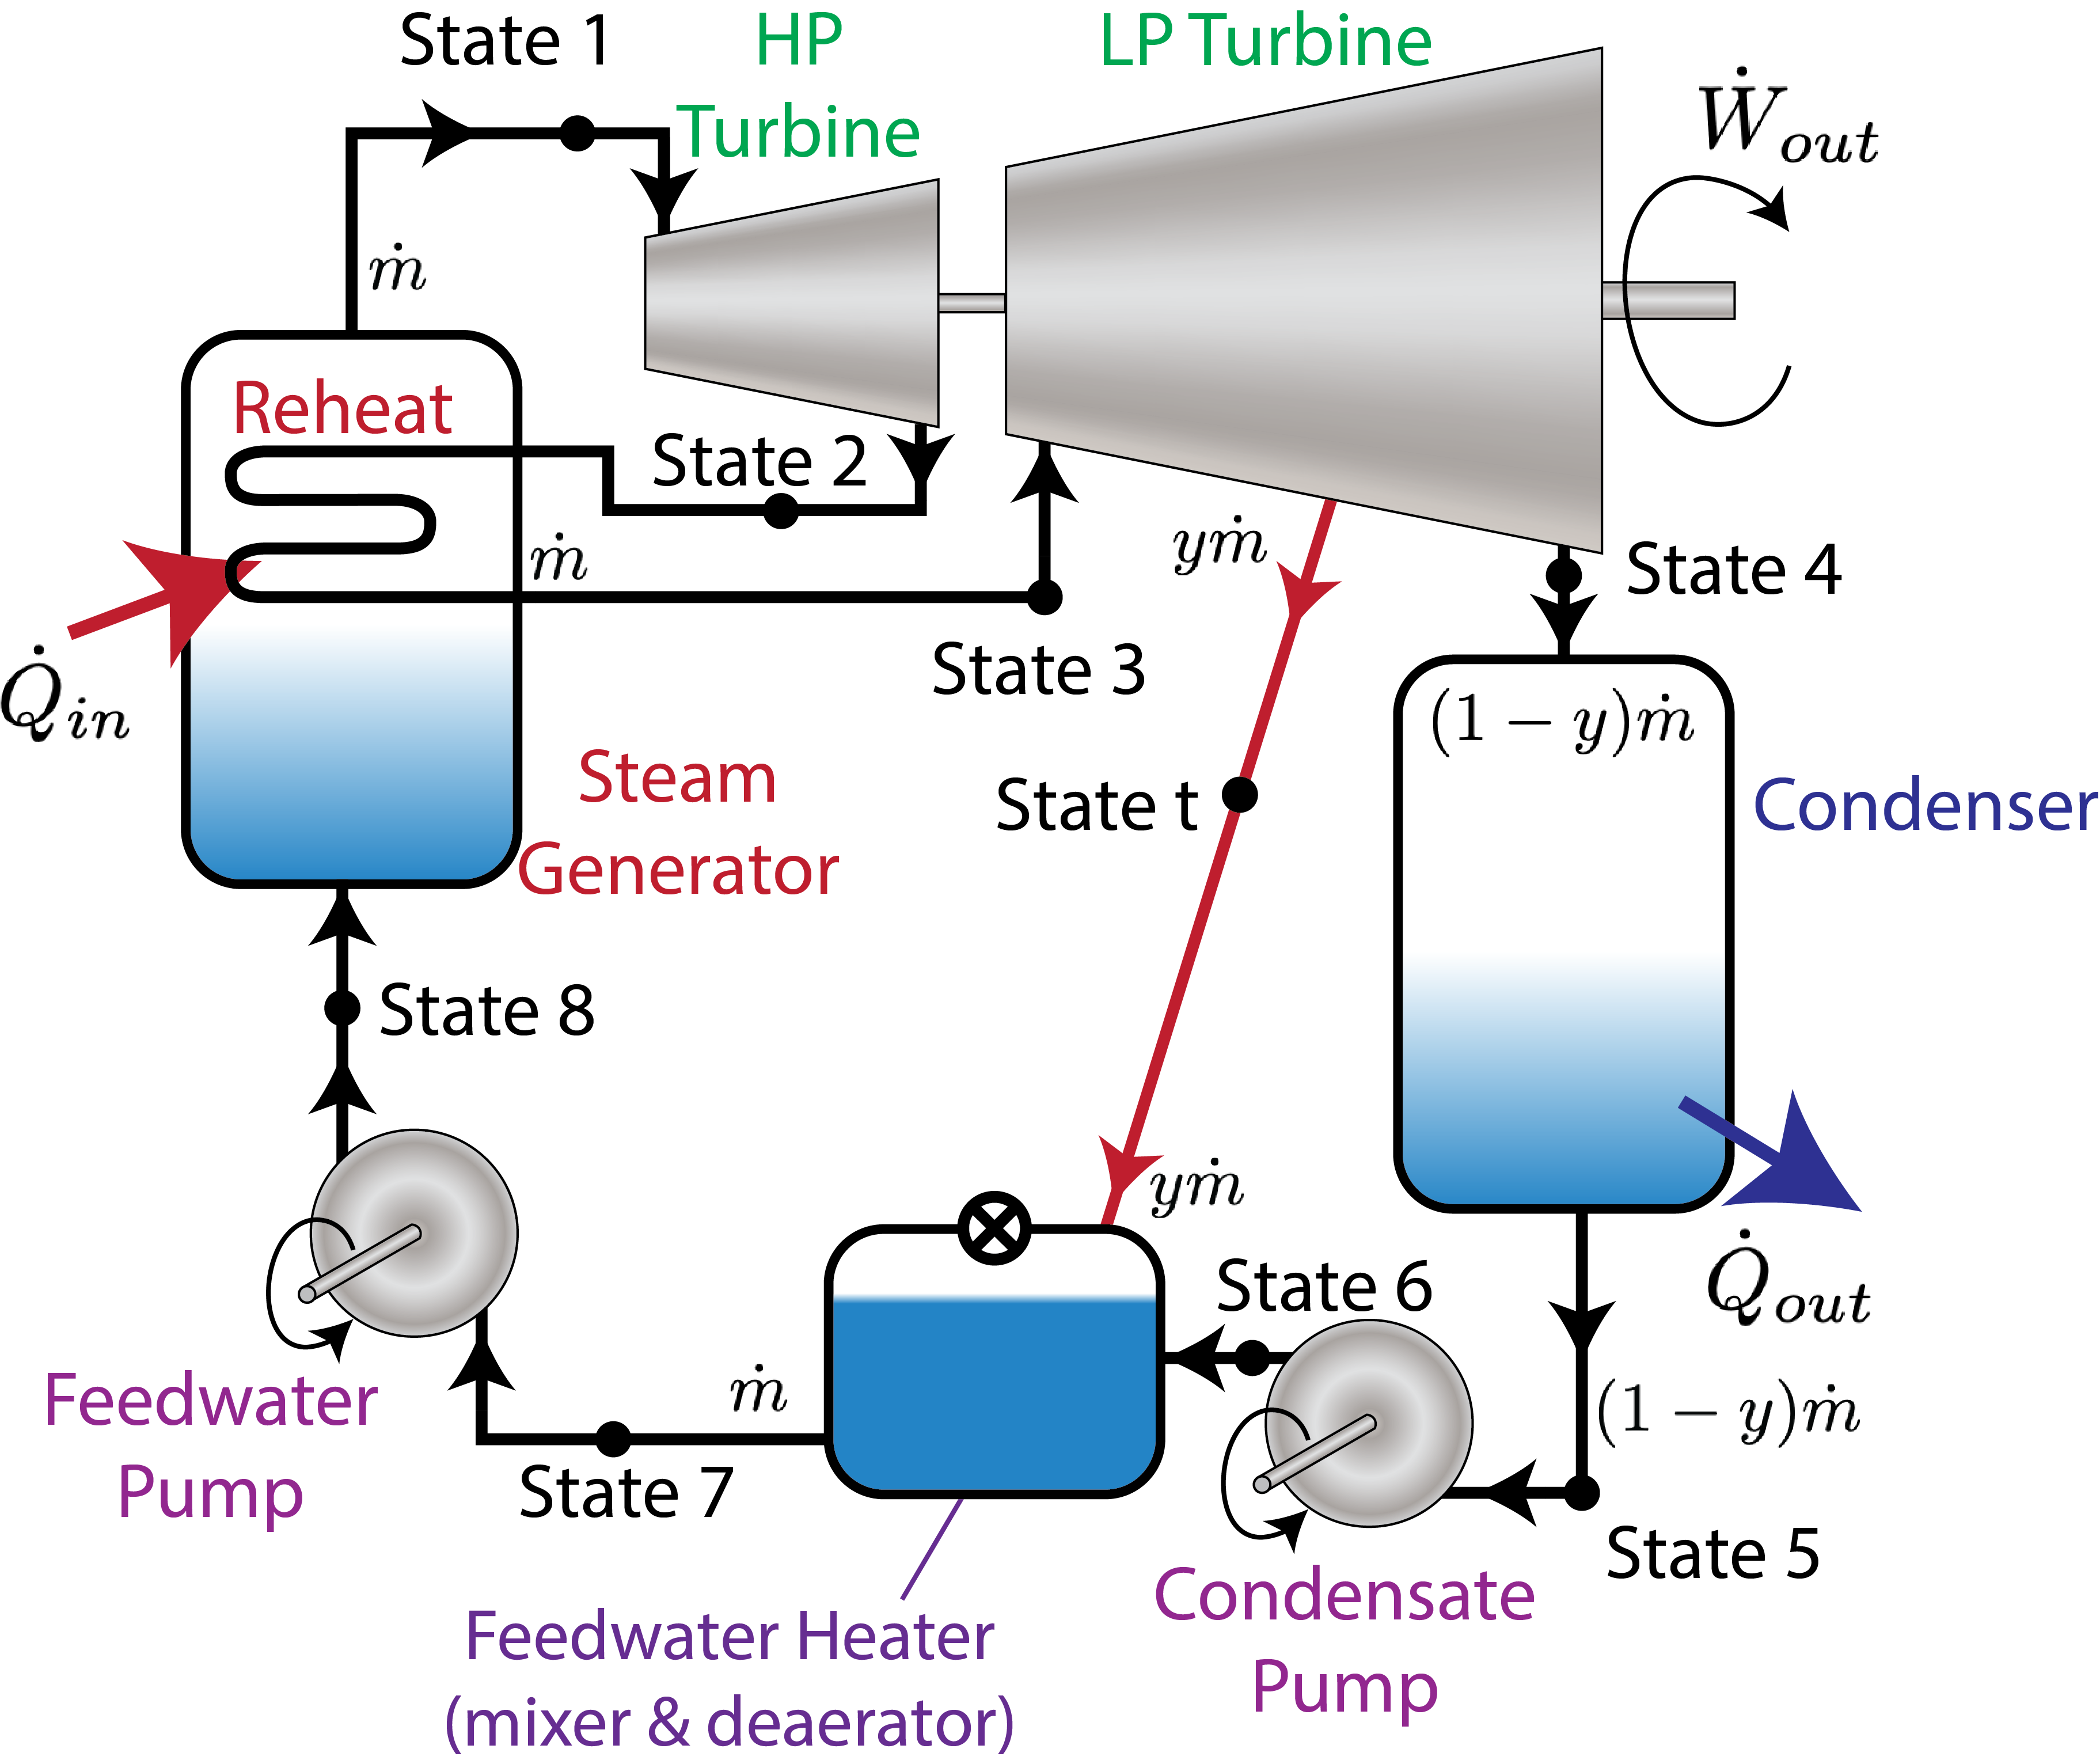
\includegraphics[width=0.75\textwidth]{RankineWithRegen}
    %\captionof{figure}{}
    %\label{fig:ch2_example1}
  \end{center}  

  This system is referred to as a {\bf regenerative reheat} cycle, and we will find that this simple extension of our previous system, along with the significantly higher maximum temperature, will result in an increase in thermal efficiency of the power plant.

  Note in particular the {\bf mass fraction of steam}, $y$, that is taken directly from the outlet of the HP turbine to the feedwater heater.  The remainder, $1-y$, goes through reheat, the LP turbine, and the condenser.  Also, we've changed the name of the boiler to a steam generator, since we are heating at supercritical temperatures, where boiling is not defined.

  \subsection*{Solution Methodology}
  \subsubsection*{$p$-$h$ Diagram}
  In order to build the $p$-$h$ diagram, we need to define some additional parameters.  First off, the outlet of the HP turbine will be at 1.5 MPa and 200°C.  This also sets the pressure of the LP turbine inlet and the pressure of the feedwater heater.  The outlet of the LP turbine will be at 10 kPa and 60°C.  The condenser output water at 30°C, and the feedwater heater will output saturated water.  This is sufficient to define all 8 states.
  
  \begin{center}
    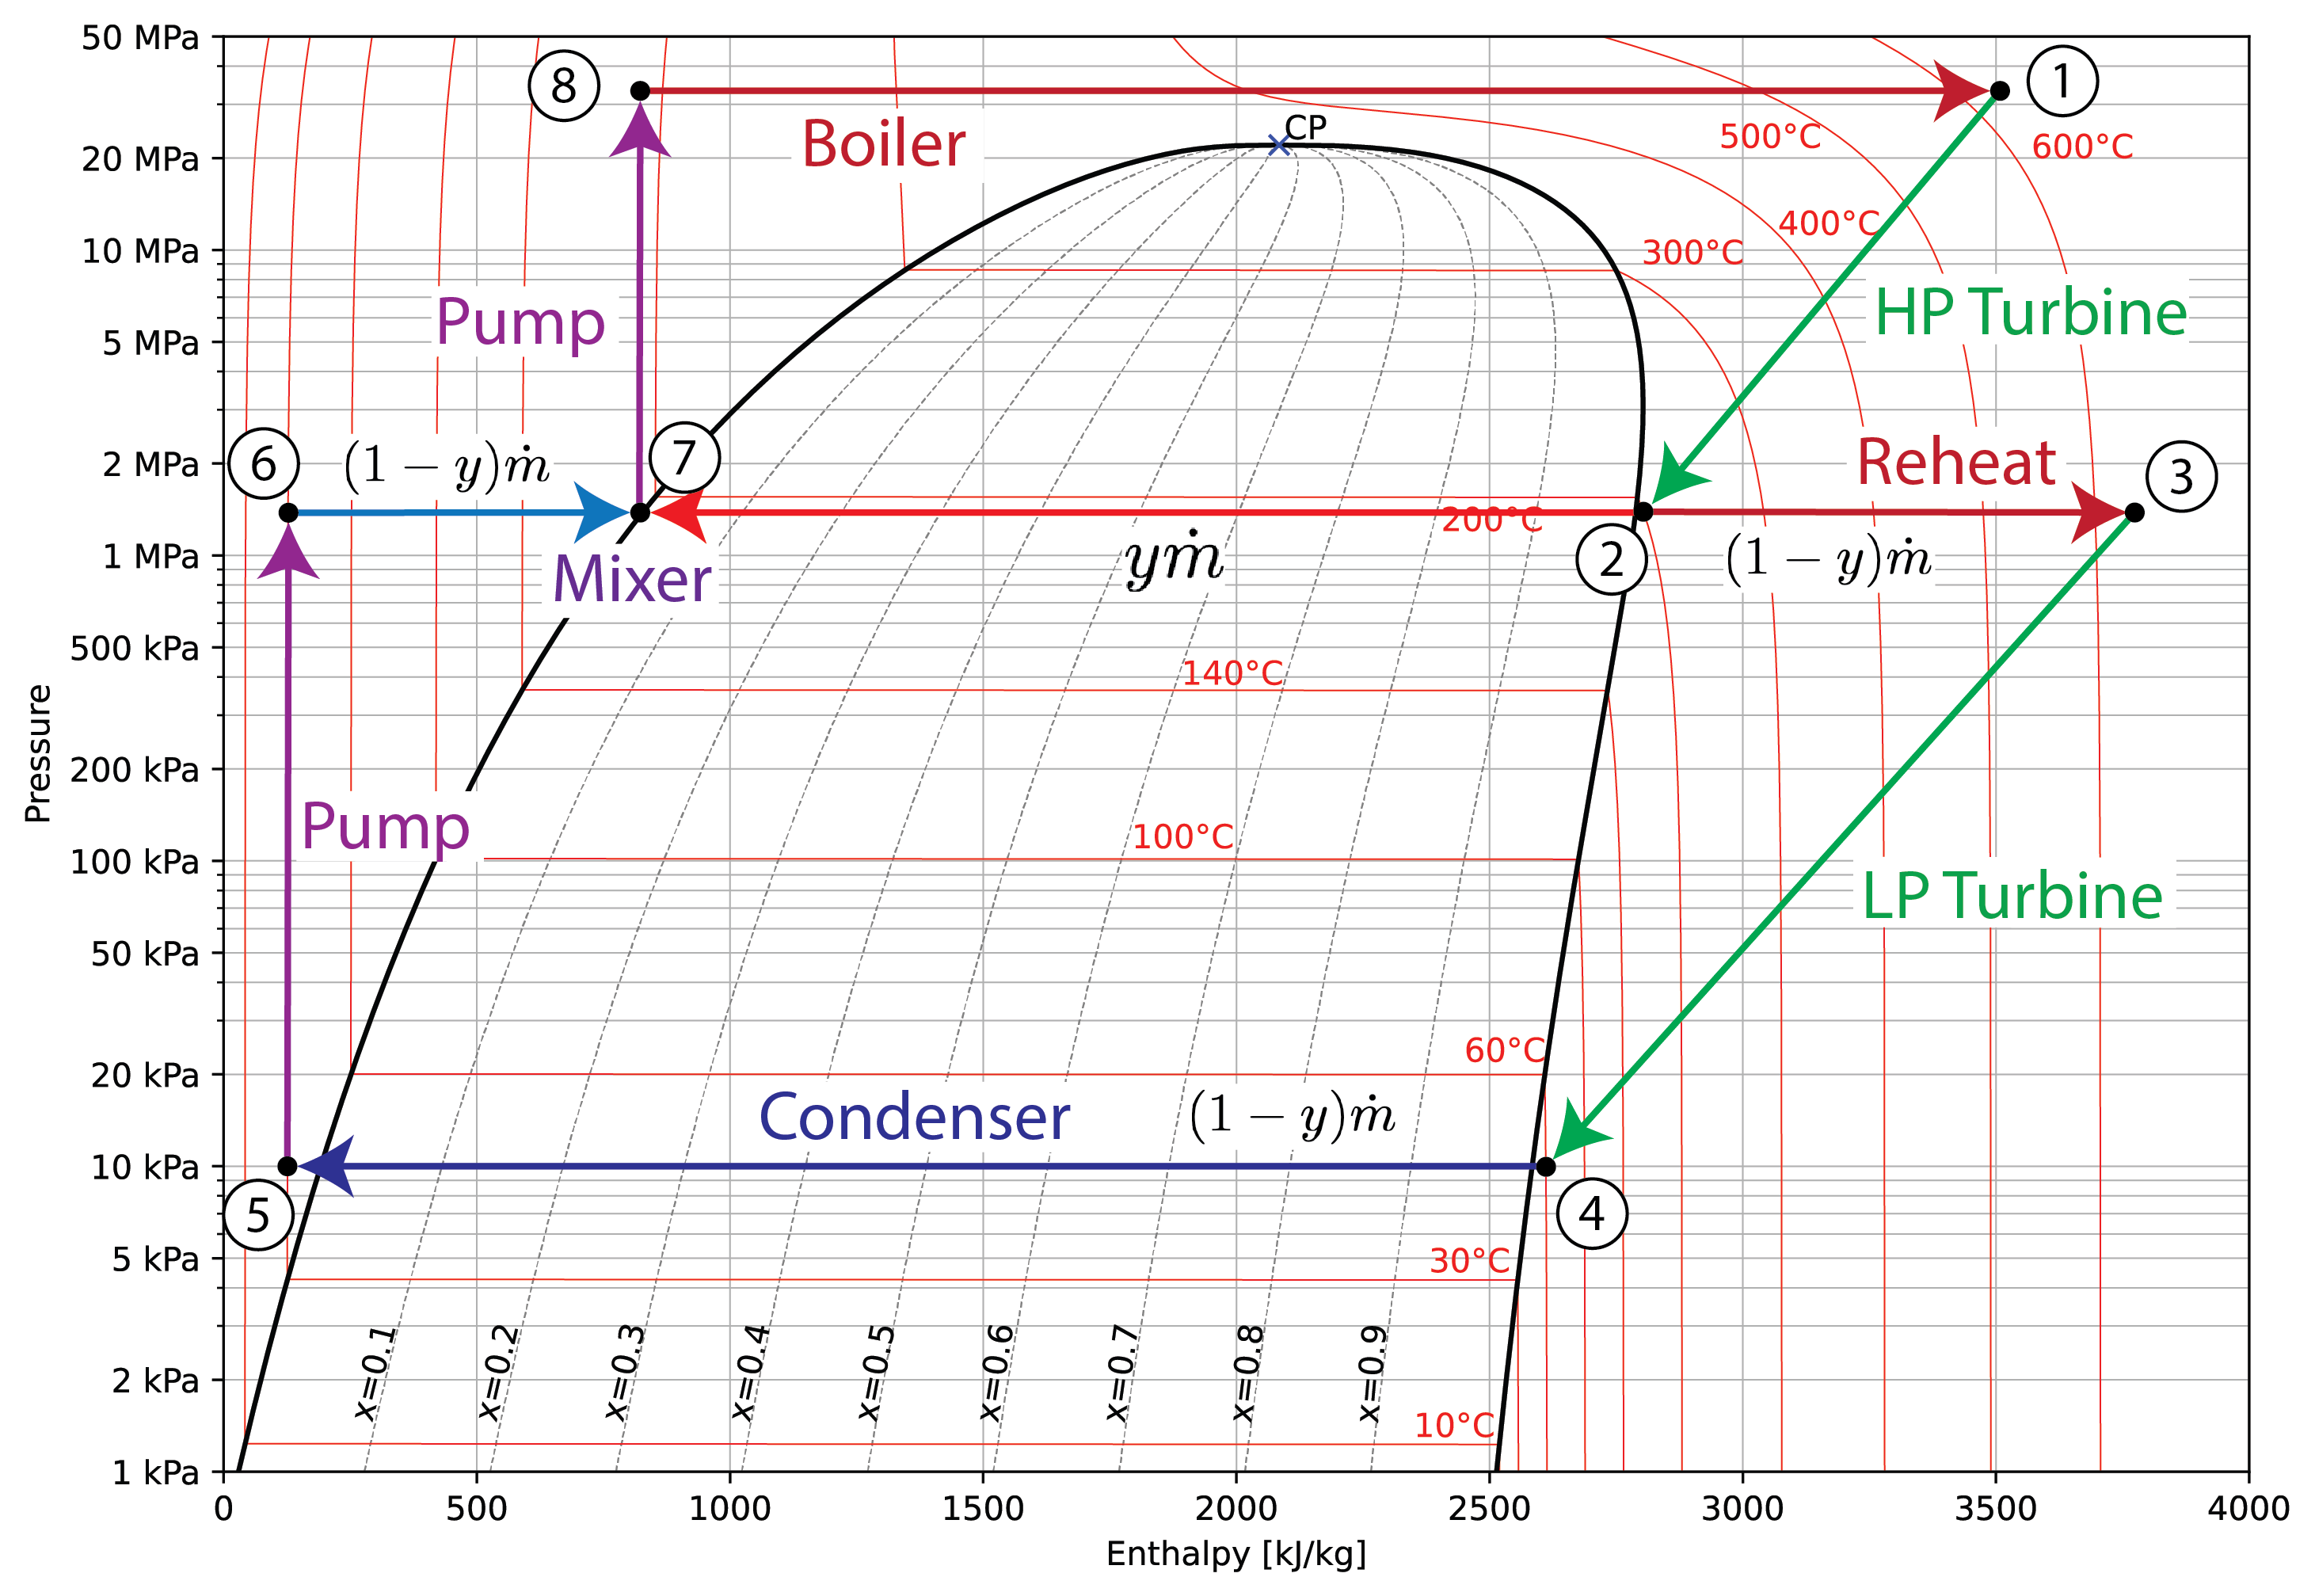
\includegraphics[width=0.9\textwidth]{RankineRegenph}
    %\captionof{figure}{}
    %\label{fig:ch2_example1}
  \end{center}

  Note that only $(1-y)\dot{m}$ of steam goes through States 3-6, while $y\dot{m}$ of steam goes directly from State 2 to 7.  This results in less work output from the LP turbine, but also significantly less energy required from the boiler.  The net effect is better thermal efficiency from the cycle as a whole.  Otherwise, we will use our state definitions to find the enthalpy of each state, and analyze the cycle in a very similar way to Examples \ref{ex:RankineCycle} and \ref{ex:ch4_supercrit}.

  \subsubsection*{Property Table}
  As in Example \ref{ex:ch4_supercrit}, most properties are simple table look-ups, often with interpolation.  States 5 and 6 require either the assumption of equivalence to saturated water at the same temperature, or evaluation with CoolProp.  The property table below was generated solely with CoolProp.  Quantities in black are taken from the problem statement, and quantities in red are calculated.
  \begin{table}[H]
    \centering
    \def\arraystretch{1.5}
    %\caption{Tabular Representation of Energy Equation for Stirling Cycle}
    %\label{tab:ch3_stirling}
    \begin{tabular}{r|cccc}
      State & Pressure & Temperature & Enthalpy & Quality \\ \hline
      1 & 33 MPa & 650°C & {\color{Red} 3576.2 $\frac{\rm kJ}{\rm kg}$} & - \\
      2 & 1.5 MPa & 200°C & {\color{Red} 2796.0 $\frac{\rm kJ}{\rm kg}$} & - \\
      3 & 1.5 MPa & 670°C & {\color{Red} 3852.6 $\frac{\rm kJ}{\rm kg}$} & - \\
      4 & 10 kPa &  60°C & {\color{Red} 2611.2 $\frac{\rm kJ}{\rm kg}$} & - \\
      5 & 10 kPa &  30°C & {\color{Red} 125.7 $\frac{\rm kJ}{\rm kg}$} & - \\
      6 & 1.5 MPa & 30°C & {\color{Red} 127.1 $\frac{\rm kJ}{\rm kg}$} & - \\
      7 & 1.5 MPa & {\color{Red} 198°C} & {\color{Red} 844.6 $\frac{\rm kJ}{\rm kg}$} & 0.0 \\
      8 & 33 MPa & {\color{Red} 198°C} & {\color{Red} 859.1 $\frac{\rm kJ}{\rm kg}$} & - \\
    \end{tabular}
    \def\arraystretch{1.0}
  \end{table}
  We can check these values against the approximate locations of the States in the $p$-$h$ diagram, and we see that each of the enthalpies is reasonable.

  \subsubsection*{Finding $y$}
  The big unknown of the analysis at this point is the mass fraction of steam that goes directly from State 2 to State 7.  In order to perform this analysis, we look at Equation \ref{eq:ch4_mixer}:
  \begin{align*}
    \dot{m}_{out} h_{out} &= \sum \dot{m}_{in} h_{in} \\
    \cancel{\dot{m}}\, h_7 &= y \cancel{\dot{m}}\, h_2 + (1-y)\cancel{\dot{m}}\,h_6 \\
    h_7 - h_6 &= y(h_2 - h_6) \\
    y &= \frac{h_7 - h_6}{h_2-h_6}
  \end{align*}
  Plugging in values here gives us the following:
  \begin{equation*}
    y = \frac{844.6\ \frac{\rm kJ}{\rm kg} - 127.1\ \frac{\rm kJ}{\rm kg}}{2796.0\ \frac{\rm kJ}{\rm kg}-127.1\ \frac{\rm kJ}{\rm kg}} = \redbox{0.269 = 26.9\%}
  \end{equation*}
  Thus, 26.9\% of the steam is diverted to the mixer, while 73.1\% is reheated and sent to the LP turbine.

  \subsubsection*{Turbine/Pump Work, Boiler/Reheat/Condenser Heat Transfer}
  The analysis here is nearly identical to that done in Example \ref{ex:ch4_supercrit}, with the exception of some change in State numbers for the pumps.  Additionally, we will wait to lump together the turbines and heats until we can calculate the mass flow rates of steam through each component.

  The turbines are found through the difference in enthalpies:
  \begin{align*}
    w_{HPT} &= h_1 - h_2 = 3576.2\ \frac{\rm kJ}{\rm kg} - 2796.0\ \frac{\rm kJ}{\rm kg} = \redbox{780.2\ \frac{\rm kJ}{\rm kg}} \\
    w_{LPT} &= h_3 - h_4 = 3852.6\ \frac{\rm kJ}{\rm kg} - 2611.2\ \frac{\rm kJ}{\rm kg} = \redbox{1241.4\ \frac{\rm kJ}{\rm kg}}
  \end{align*}

  The pumps can be found the same way:
  \begin{align*}
    w_{pump, 5-6} &= h_6 - h_5 = 127.1\ \frac{\rm kJ}{\rm kg} - 125.7\ \frac{\rm kJ}{\rm kg} = \redbox{1.4\ \frac{\rm kJ}{\rm kg}} \\
    w_{pump, 7-8} &= h_8 - h_7 = 859.1\ \frac{\rm kJ}{\rm kg} - 844.6\ \frac{\rm kJ}{\rm kg} = \redbox{14.5\ \frac{\rm kJ}{\rm kg}}
  \end{align*}

  Again, we could use Equation \ref{eq:ch4_pumpEnthalpy}, though we choose to skip that analysis for this cycle.
  
  There is no work that occurs in the boiler or reheat cycle, meaning we can again use the difference in enthalpy:
  \begin{align*}
    q_{boiler} &= h_1 - h_8 = 3576.2\ \frac{\rm kJ}{\rm kg} - 859.1\ \frac{\rm kJ}{\rm kg} = \redbox{2717.1\ \frac{\rm kJ}{\rm kg}} \\
    q_{reheat} &= h_3 - h_2 = 3852.6\ \frac{\rm kJ}{\rm kg} - 2796.0\ \frac{\rm kJ}{\rm kg} = \redbox{1056.6\ \frac{\rm kJ}{\rm kg}}
  \end{align*}

  Finally, we can calculate the heat transfer in the condenser, again assuming no work occurs:
   \begin{equation*}
    q_{cond} = h_4 - h_5 = 2611.2\ \frac{\rm kJ}{\rm kg} - 125.7\ \frac{\rm kJ}{\rm kg} = \redbox{2485.5\ \frac{\rm kJ}{\rm kg}}
   \end{equation*}

   \subsubsection*{Mass Flow Rates of Steam, Efficiency, and Total Heat Transfer}
   The total mass flow rate, $\dot{m}$, must be sufficient to provide 1,000 MW of net power.  We can calculate the net power, accounting for the mass fraction of steam that bypasses the LP Turbine, as follows:
   \begin{equation*}
     \dot{W}_{net} = \dot{m}\:w_{HPT} + (1-y)\dot{m}\,w_{LPT} - (1-y)\dot{m}\,w_{pump, 5-6} - \dot{m}\,w_{pump, 7-8}
   \end{equation*}
   Thus, we are looking at the mass flow rate through each component to determine its contribution to the net work.  Alternatively, we could define $\dot{W}_{net} = \dot{m} w_{net}$, and calculate the following:
   \begin{equation*}
     w_{net} = \frac{\dot{W}_{net}}{\dot{m}}=w_{HPT} + (1-y)w_{LPT} - (1-y)w_{pump, 5-6} - w_{pump, 7-8}
   \end{equation*}
   Plugging in numbers, we get the following:
   \begin{equation*}
      w_{net} = 780.2\ \frac{\rm kJ}{\rm kg} + 0.731 \left(1241.4\ \frac{\rm kJ}{\rm kg}\right) - 0.731 \left(1.4\ \frac{\rm kJ}{\rm kg}\right) - 14.5\ \frac{\rm kJ}{\rm kg} = \redbox{1672.1\ \frac{\rm kJ}{\rm kg}}
   \end{equation*}

   Calculating $\dot{m}$ is now trivial:
   \begin{equation*}
    \dot{m} = \frac{\dot{W}_{net}}{w_{net}} = \frac{1,000\ \rm MW}{1672.1\ \frac{\rm kJ}{\rm kg}} = \redbox{598.1\ \frac{\rm kg}{\rm s}}
   \end{equation*}

   Defining $\dot{Q}_{in} = \dot{m}\,q_{in} = \dot{m}\,q_{boiler}+(1-y)\dot{m}\,q_{reheat}$, we calculate the following for $q_{in}$:
   \begin{equation*}
     q_{in} = q_{boiler} + (1-y)q_{reheat} = 2717.1\ \frac{\rm kJ}{\rm kg} + 0.731 \left(1056.6\ \frac{\rm kJ}{\rm kg}\right) = \redbox{3489.5\ \frac{\rm kJ}{\rm kg}}
   \end{equation*}
   This allows us to calculate our efficiency:
   \begin{equation*}
     \eta_{th} = \frac{w_{net}}{q_{in}} = \frac{1672.1\ \frac{\rm kJ}{\rm kg}}{3489.5\ \frac{\rm kJ}{\rm kg}} = 0.479 = \redbox{47.9\%}
   \end{equation*}
   This is greatly improved from the efficiencies found in the previous examples of this chapter.

   As a side-note, if we had chosen to forego the feedwater heater, we would have increased $w_{net}$ to $2005.7\ \frac{\rm kJ}{\rm kg}$, due to the increased mass flow rate in the LP turbine. However, we would have simultaneously increased $q_{in}$ to $4491.2\ \frac{\rm kJ}{\rm kg}$, because of the increased heating load on the boiler, as well as the increased mass flow rate through the re-heater.  Without the feedwater heater, the cycle would have had an efficiency of only 44.7\% (which is still much better than the previous examples).

   Finally, we will look at the total heat transfer required from the boiler and re-heater.
   \begin{equation*}
     \dot{Q}_{in} = \dot{m}\, q_{in} = \left(598.1\ \frac{\rm kg}{\rm s}\right)\left(3489.5\ \frac{\rm kJ}{\rm kg}\right) = \redbox{2.087\ \rm GW}
   \end{equation*}
   Assuming perfect combustion, this requires 72 kg of high-quality (bituminous) coal a second, or 6200 tons of coal a day.
\end{example}

% --------------------------------------------------------------------
\section{Refrigeration Cycle} \label{sec:Refrigeration}
% --------------------------------------------------------------------

\subsection{Types of Refrigerants}
% --------------------------------------------------------------------
Refrigeration cycles typically do not use air or steam.  Instead, a great deal of chemical research is focused around finding substances that have $p$-$h$ curves that are significantly more conducive to the refrigeration cycle.

In the early days of refrigeration, the two refrigerants in common use were ammonia and carbon dioxide. Both were problematic - ammonia is toxic and carbon dioxide requires extremely high pressures and pressures (roughly 100 atmospheres and 160°C).

In the last century or so, a large number of different refrigerants have been manufactured.  The Heating, Refrigeration, and Air Conditioning Institute of Canada maintains a \href{https://www.hrai.ca/uploads/userfiles/files/refrigerant_table_June2019.pdf}{list of refrigerants} with possible uses and dangers, including flammability, toxicity, and possible damage to the environment.

\subsubsection{R12 (Phase-out started 1989) / R22 (Phase-out started 2010)}
When the refrigerant R12 (dichloro-diflouro-methane) was discovered it took over as the refrigerant of choice. It is an extremely stable, non-toxic fluid, and it operates at pressures always somewhat higher than atmospheric, so that if any leakage occurred, air would not leak into the system.  Thus, a technician can recharge a refrigeration system without having to apply vacuum.

Unfortunately when the refrigerant does ultimately leak, it will make its way up to the ozone layer. The ultraviolet radiation from the sun breaks up the molecule, it releases the highly active chlorine radicals, which deplete the ozone layer. Because of this environmental problem, R12 and other chloro-fluoro-carbons (CFCs) have since been banned from usage on a global scale.

For home air conditioning, most new units starting in the 1980s were using R22, which became the standard as Freon 12 was phased out.  R22 has 5\% of the ozone depletion potential of R12, but this is still considered too high for safe use.  Currently, R22 cannot be produced or imported, and current units using R22 must rely on recycled or stockpiled materials.

\subsubsection{R134a (Phase-out started 2021) / R410a (Phase-out starts 2025)}
In order to replace R12, chlorine free R134a (tetraflouro-ethane) was introduced for automotive air conditioners.  R410a has been the most common replacement for R22 in residential HVAC systems in the last decade.  Neither R134a nor R410a is known to cause ozone depletion.

Recently, however, the international scientific consensus is that Global Warming is caused by human energy related activity, and various man made substances are defined on the basis of Global Warming Potential (GWP) with reference to carbon dioxide (GWP=1).

R134a has been found to have a GWP of 1300 and, as of model year 2021, automobile air conditioning systems will be barred from using R134a as a refrigerant.  Likewise, R410a has a GWP of 2088, and has a phasedown beginning in 2025.

\subsubsection{Replacements for R134a}
The option to replace R134a that has been adopted by most car manufacturers is the refrigerant R1234yf.  R1234yf has a GWP of around 1 (roughly the same global warming potential as carbon dioxide), but is somewhat flammable.  The risk of fire due to the refrigerant is negligible, but additional safety requirements have been set in place \href{https://www.epa.gov/mvac/refrigerant-transition-environmental-impacts}{by the EPA}.

Alternatively, a return to carbon dioxide (R744) is suggested.  As mentioned before, this requires a much higher pressure than other refrigerants, and results in a much higher compressor temperature.  There are no vehicles currently using R744, but several foreign automobile manufacturers are exploring its use.

\subsubsection{Replacements for R410a}
New residential air conditioning systems are changing from R410a to R32.  Like R1234yf, R32 has a lower GWP (around 677).  Ironically, R410a is a mixture that contains R32 and R125.  R32 requires a slightly higher pressure than R410a, but significantly less refrigerant.  While this is an improvement over R410a, it will likely be phased out in the next several decades as research into refrigerants with lower GWP continues.


\subsection{Refrigeration}
% --------------------------------------------------------------------
\begin{figure}[H]
\centering
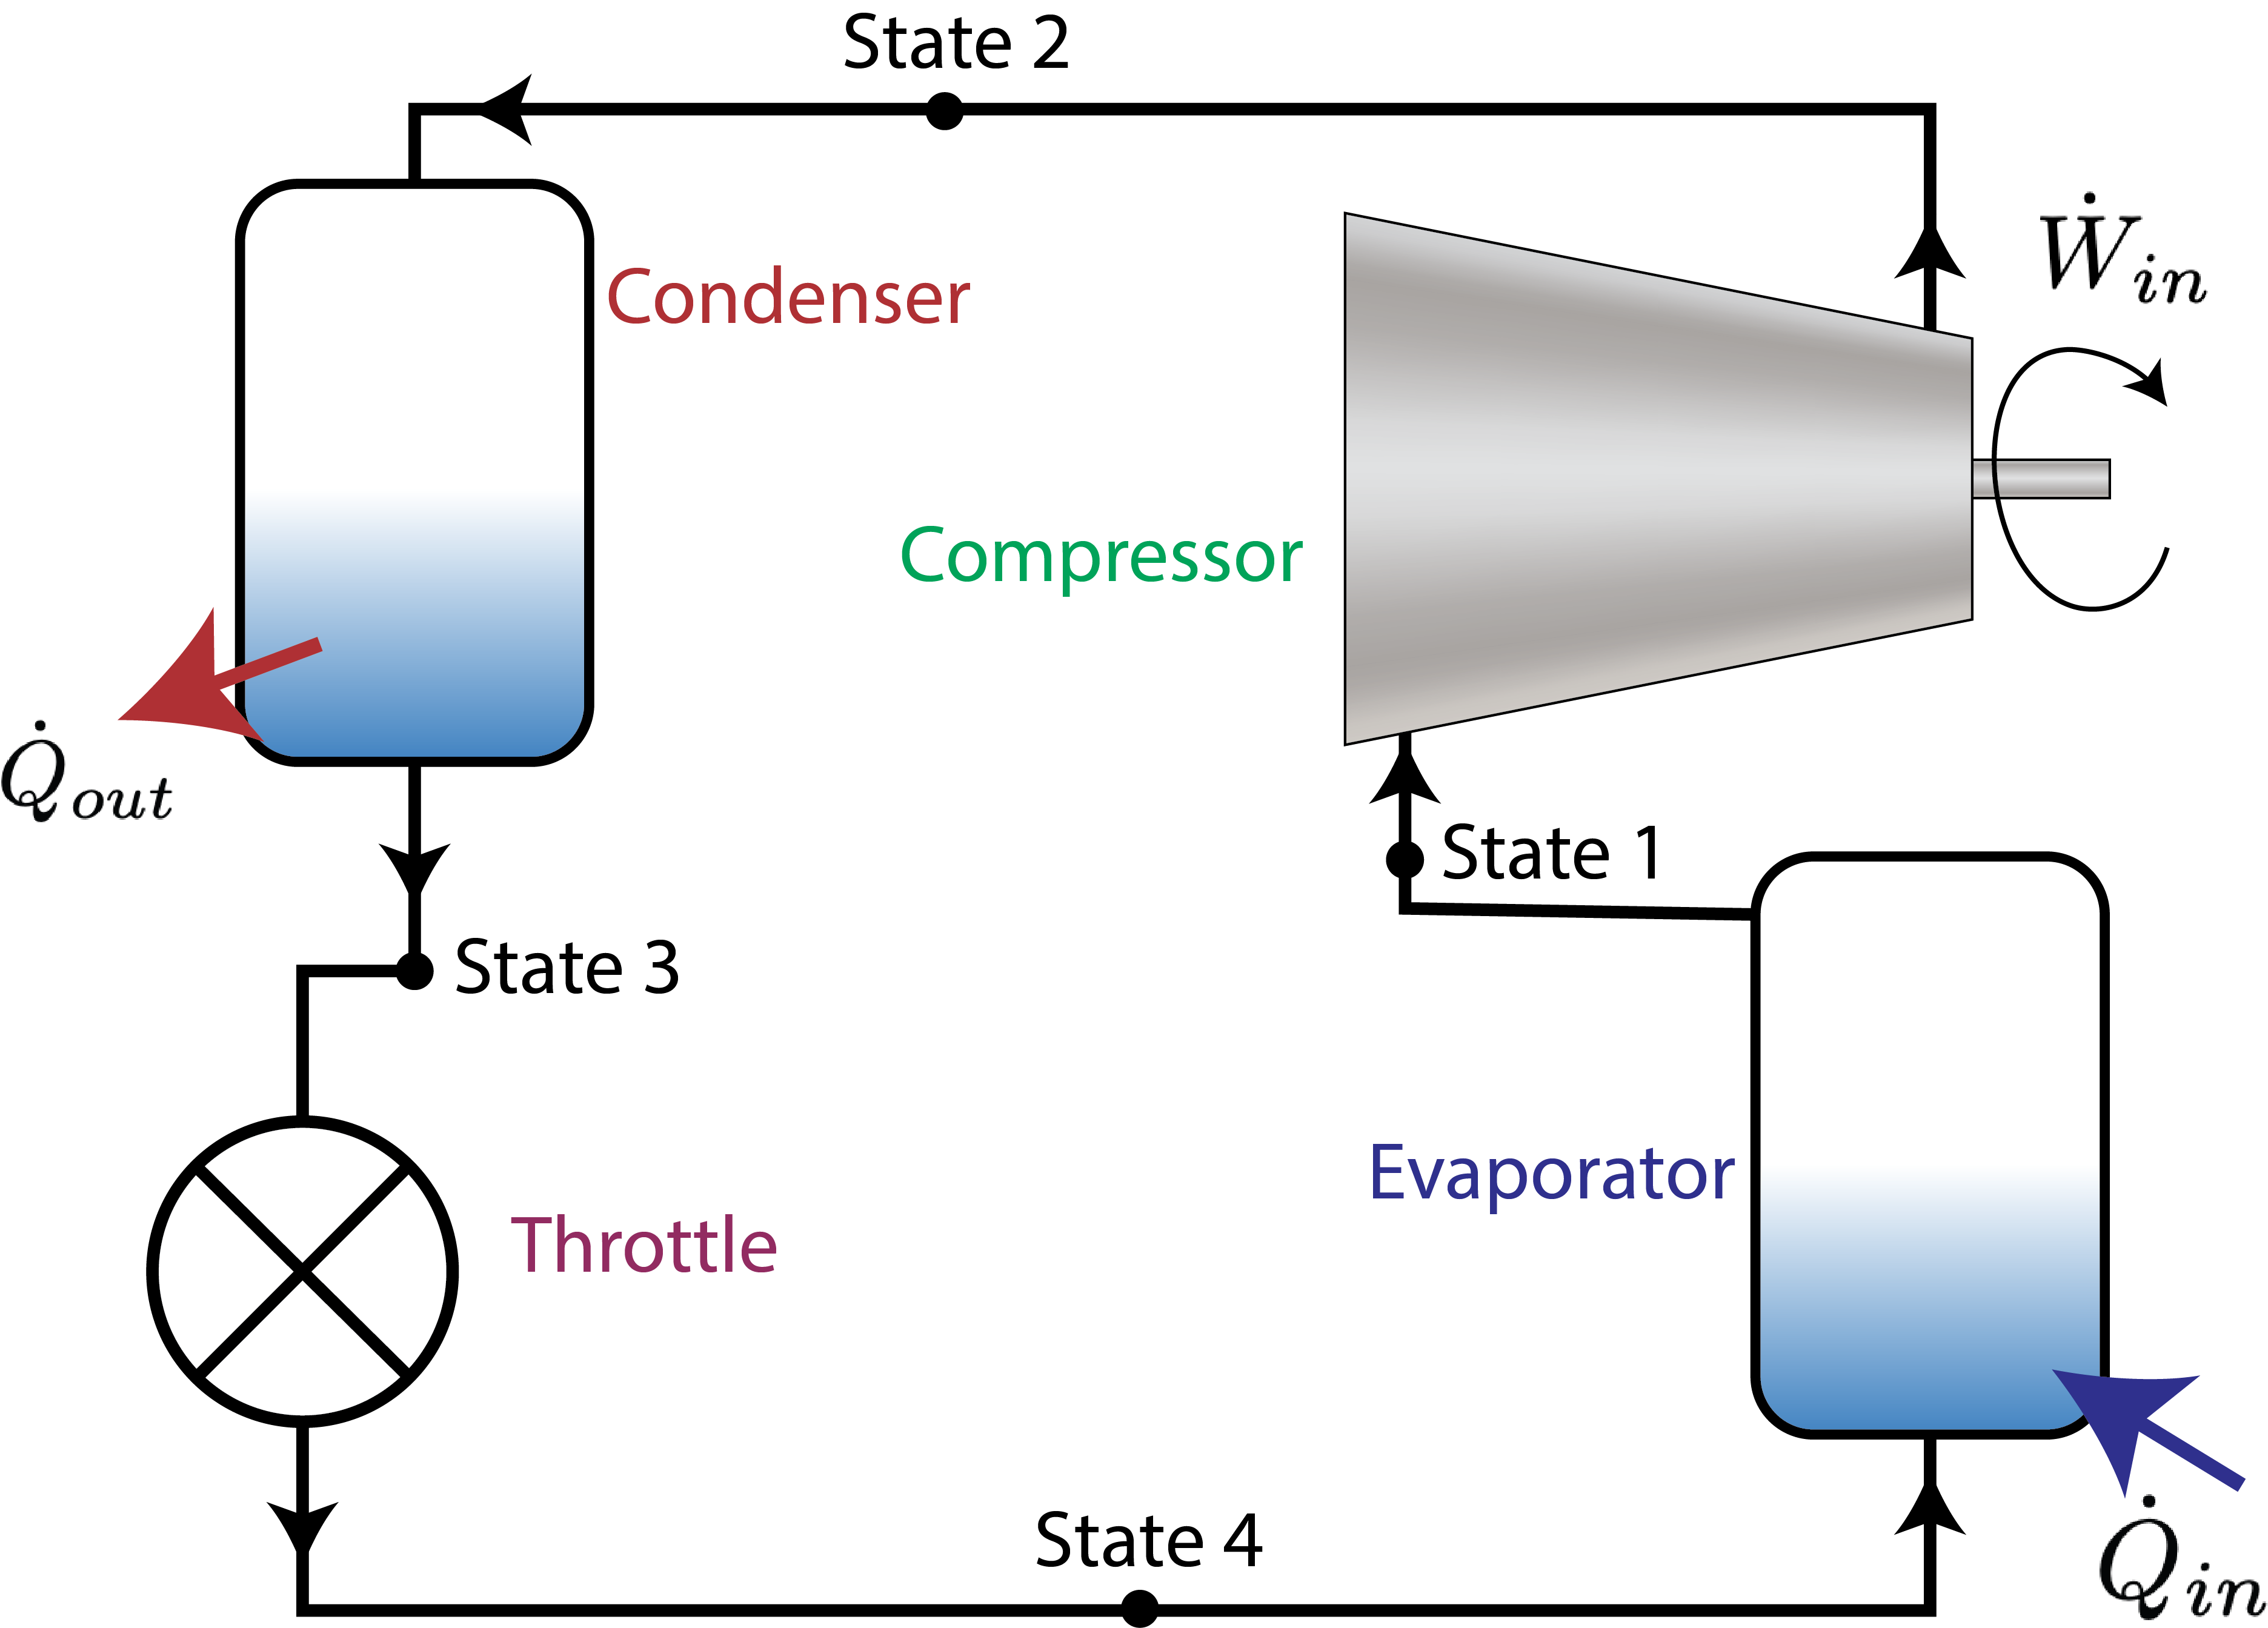
\includegraphics[width=0.75\textwidth]{RefrigerationDiagram}
\caption{Diagram describing the refrigeration cycle.}
\label{fig:ch4_RefrigerationCycle}
\end{figure}

Refrigeration cycles typically consist of a compressor, condenser, throttle, and evaporator.  State 1 begins at low temperature, immediately before the compressor.  Work is applied through the compressor in Process 1-2, which increases the pressure and temperature, and also provides the energy to move the fluid through the cycle (see Section \ref{sec:ch4_pumps}).  State 2 is the highest temperature point of the cycle.  In Process 2-3, heat is extracted from the system (added to the environment) at high temperature from the condenser (see Section \ref{sec:ch4_condensers}).  State 3 is either saturated liquid or supercooled liquid.  The throttle reduces the pressure across Process 3-4, similar to a turbine, but with no work extracted (see Section \ref{sec:ch4_throttles}).  State 4 is a mixture of liquid and vapor at low pressure and temperature.  The evaporator in Process 4-1 adds heat to the system (extracts heat from the environment) at low temperature (see Section \ref{sec:ch4_boilers}), and brings the system back to State 1.

As in the Rankine Cycle, only heat transfer occurs in the evaporator and condenser, as there are no moving parts in those components.  The compressor is the only component that does work, and neither work nor heat transfer occurs in the throttle.

When considering efficiency, we look at the coefficient of performance, as originally defined in Section \ref{sec:ch3_StirlingCooling}.
\begin{equation*}
  COP_R = \frac{\dot{Q}_{in}}{|\dot{W}_{net}|} = \frac{q_{in}}{|w_{net}|}
\end{equation*}

The net work for the refrigeration cycle comes solely from the compressor: $w_{net} = w_{comp}$.  The heat transfer into the system (and out of the environment) comes from the evaporator, so $q_{in} = q_{evap}$.

\begin{figure}[H]
\centering
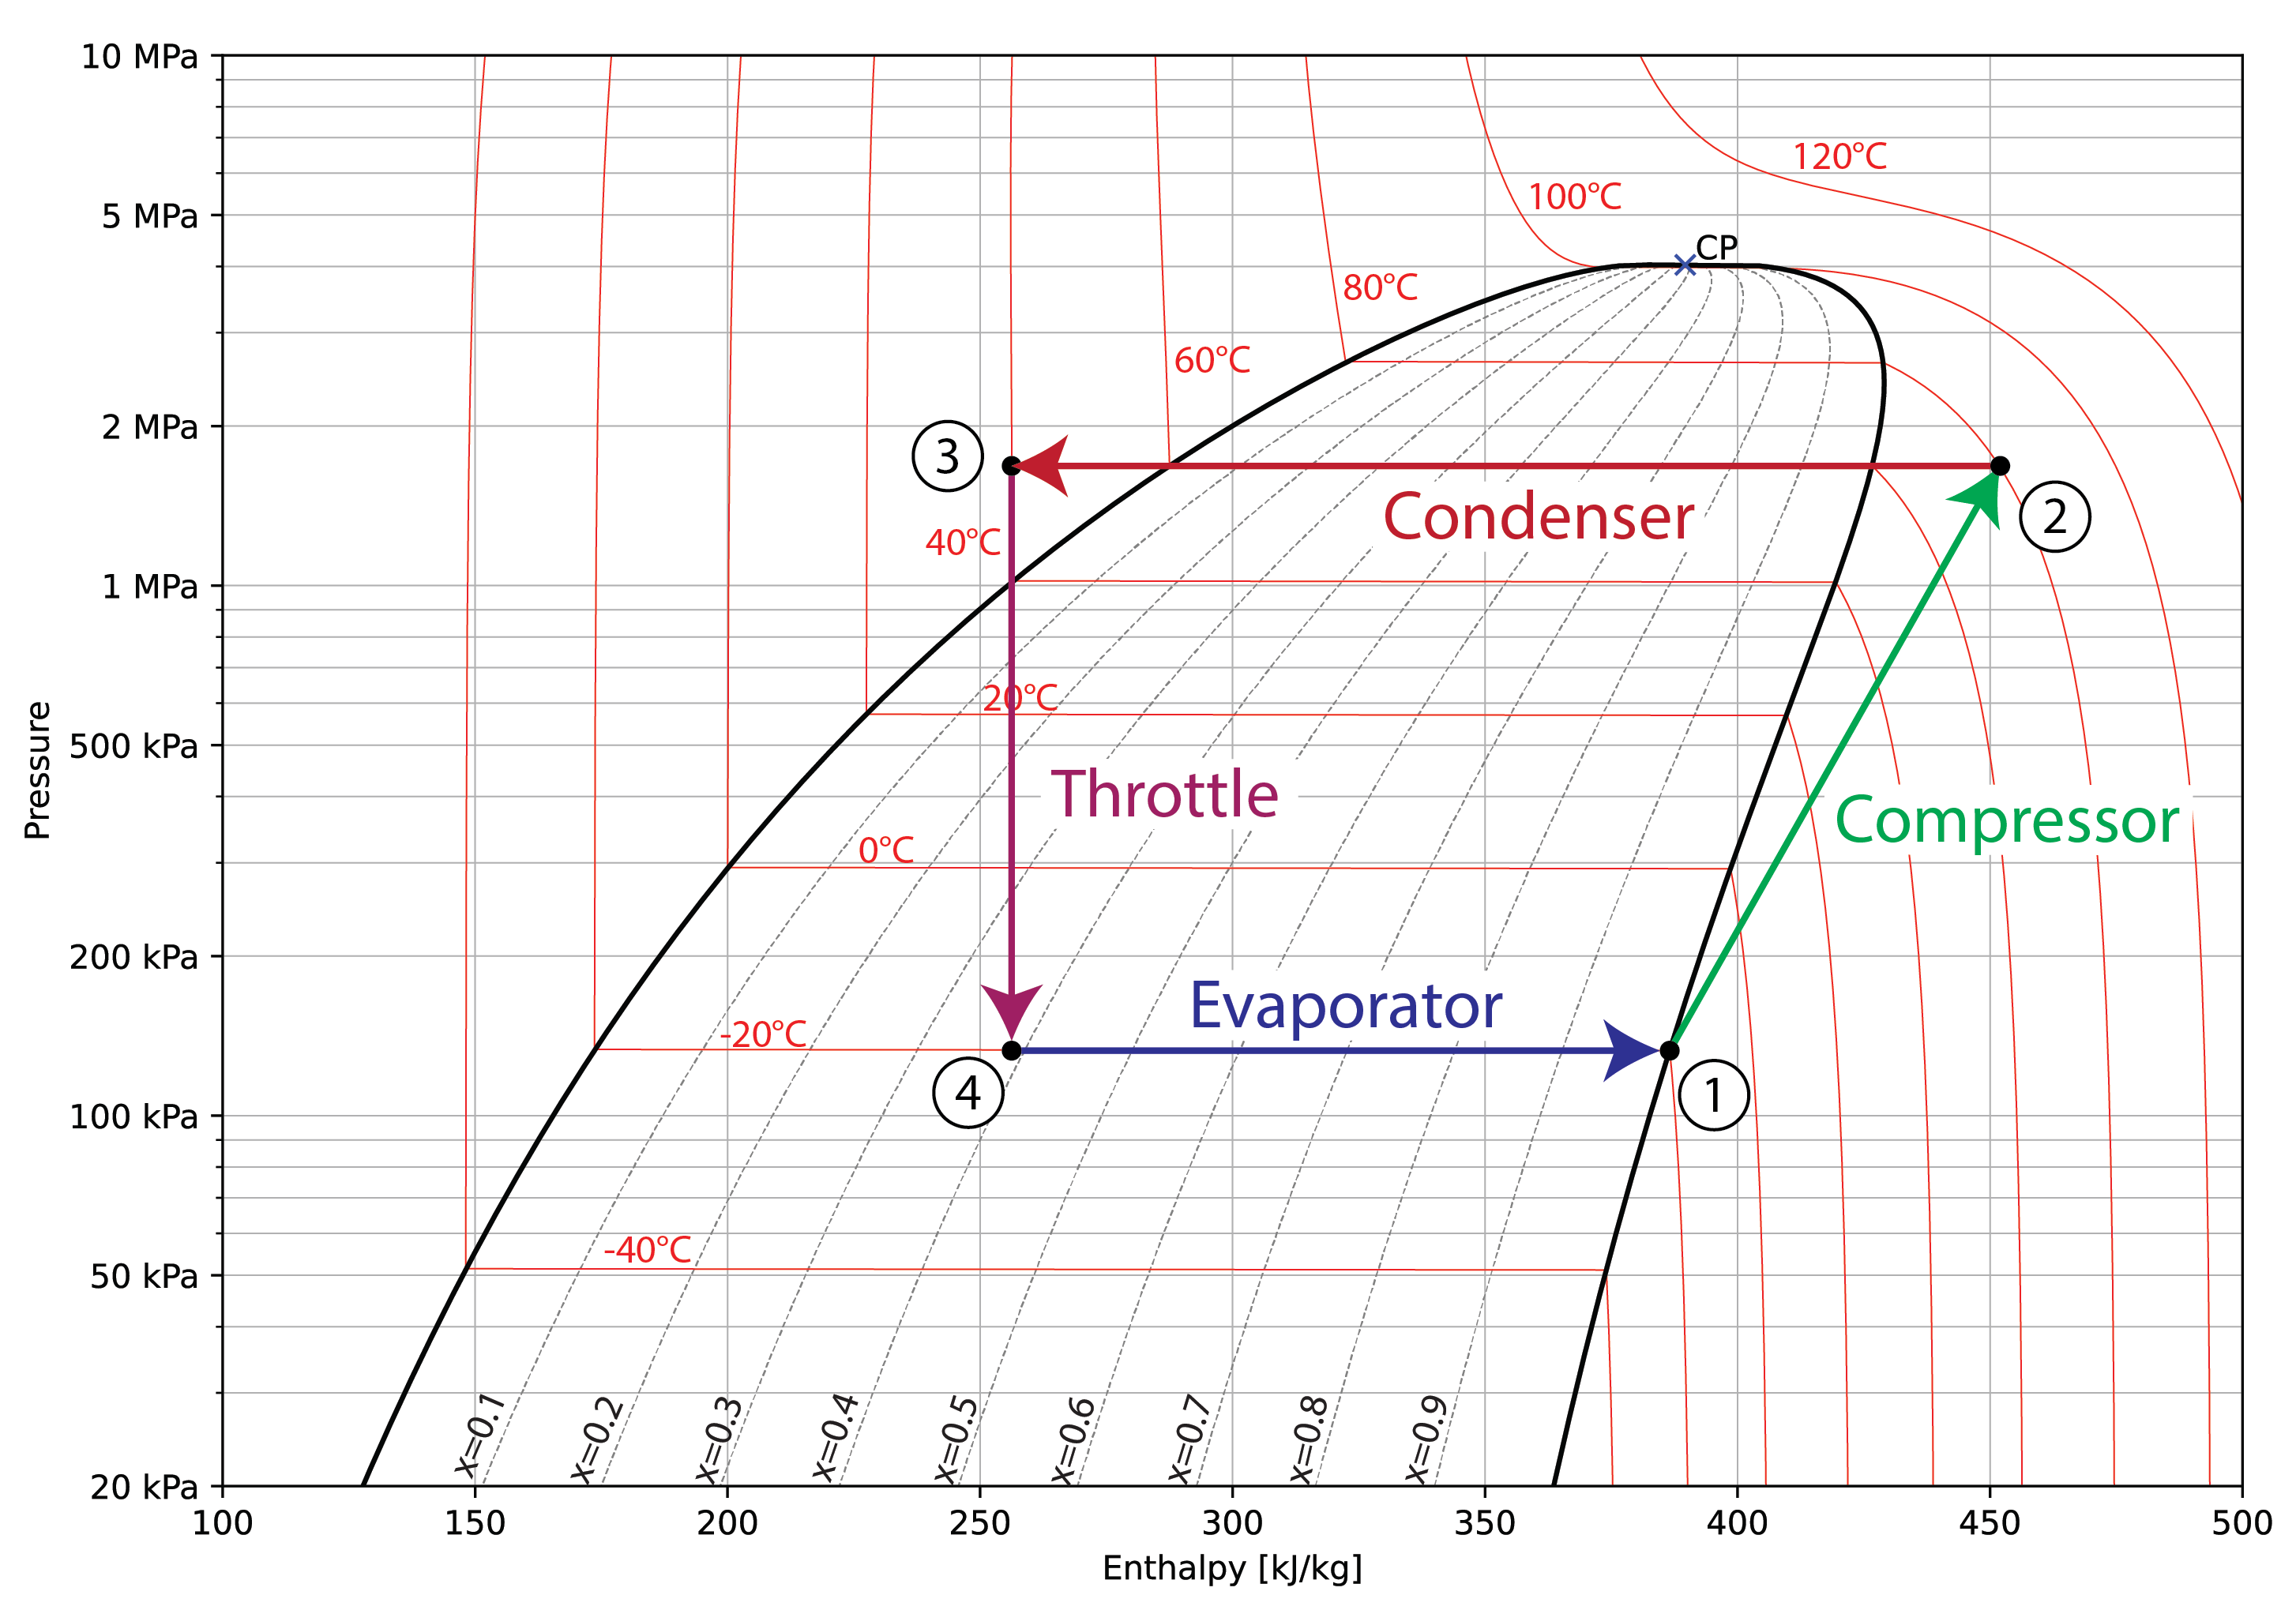
\includegraphics[width=0.9\textwidth]{Refrigerationph}
\caption{The states and processes of the refrigeration cycle shown on a $p$-$h$ diagram.}
\label{fig:ch4_Refrigerationph}
\end{figure}

Because no work occurs in the evaporation process, and no heat transfer occurs in the compressor, Equation \ref{eq:controlVolumeEnergyNoKEPE} can again be used trivially for both components:
\begin{align*}
  \dot{m} \Delta h_{1-2} &= \cancelto{0}{\dot{Q}_{1-2}} - \dot{W}_{1-2}  \quad\quad\rightarrow\quad\quad w_{comp} = h_1 - h_2 \\
  \dot{m} \Delta h_{4-1} &= \dot{Q}_{4-1} - \cancelto{0}{\dot{W}_{1-2}}  \quad\quad\rightarrow\quad\quad q_{evap} = h_1 - h_4
\end{align*}

Note that $w_{comp}$ is actually negative, as $h_2$ will be larger than $h_1$.  This makes sense, as we are spending work to effect heat transfer from cold to hot.

We can rewrite the coefficient of performance using only the state enthalpies as follows:
\begin{equation} \label{eq:ch4_COPRSimplified}
  COP_{R} = \frac{q_{evap}}{w_{comp}} = \frac{h_1-h_4}{h_2 - h_1}
\end{equation}

Note that it is possible to have a $COP$ that is greater than 1.  In fact, most residential HVAC units have $COP$ values around 4, and the $COP$ for AC units in cars is usually between 2 and 3.

The refrigeration cycle can also be used as a heat pump.  The effect of a heat pump is still to move heat from cold to hot, but in this case our goal is to heat up an already warm environment, rather than cooling an already chilled environment.  In this case, the ``output'' is the heat entering the environment from the condenser, $q_{cond}$.

In this case, we find that the coefficient of performance is as follows:
\begin{equation} \label{eq:ch4_COPHPSimplified}
  COP_{HP} = \frac{q_{cond}}{w_{comp}} = \frac{h_2-h_3}{h_2 - h_1}
\end{equation}

The coefficient of performance for a heat pump will always be exactly 1 greater than that for a refrigerator ($COP_{HP} = COP_R + 1$).

Example \ref{ex:ch4_refrigeration} contains an more detailed analysis of a simple refrigeration system.

\begin{example}[label=ex:ch4_refrigeration]{A Basic R134a Vapor-Compression Refrigeration System}
  A residential HVAC system uses R134a to transport heat out of the cooled living space and into the warmer outdoor environment.  The refrigerant will be 60°C leaving the compressor (hot enough to lose heat to the environment on a hot summer day), and 5°C entering the evaporator (cold enough to take heat from the indoor space, but warm enough to avoid collecting freezing water vapor on the evaporator coils).
  The pressure in the condenser will be 1.2 MPa, the temperature leaving the condenser will be slightly supercooled at 40°C, and the temperature leaving the evaporator will be slightly superheated at 10°C.
  Using this information, do the following:
  \begin{enumerate}[a)]
    
  \item draw each of the states and processes on the $p$-$h$ diagram for R134a

  \item find the power of the compressor

  \item find the heat transfer rates of the evaporator and condenser

  \item calculate the coefficient of performance (COP) of the system, either as a refrigerator or as a heat pump
  \end{enumerate}

  \subsection*{Solution Methodology}
  As before, we will use the information provided in order to plot the states and processes on the $p$-$h$ diagram (this time for R134a).  Once we have the diagram, we will find the enthalpy of each state using either CoolProp or interpolation from tables.  Finally, we can find the various power and heat transfer rates, which will lead to the coefficient of performance.

  \subsubsection*{$p$-$h$ Diagram}

  In order to plot the $p$-$h$ diagram, we do need some additional properties:
  \begin{itemize}
  \item The temperature of State 1 is defined as 10°C, but we need to find the pressure in the evaporator.
  \item State 2 is fully defined, with a pressure equal to the condenser pressure of 1.2 MPa, and the outlet temperature of the compressor defined as 60°C.
  \item State 3 is fully defined, again using the condenser pressure, but with a temperature of 40°C.
  \item State 4 again needs the pressure in the evaporator, though we know the temperature is 5°C.
  \end{itemize}

  The pressure inside the condenser is related to the temperature of state 4, as it is a saturated liquid-gas mixture.  We can therefore find the pressure from Appendix \ref{sec:R134aSatT}.  Some quick interpolation gives us $p_4 = p_1 = 350$ kPa.  With that, everything is defined, and we can create the diagram.

  \begin{figure}[H]
    \centering
    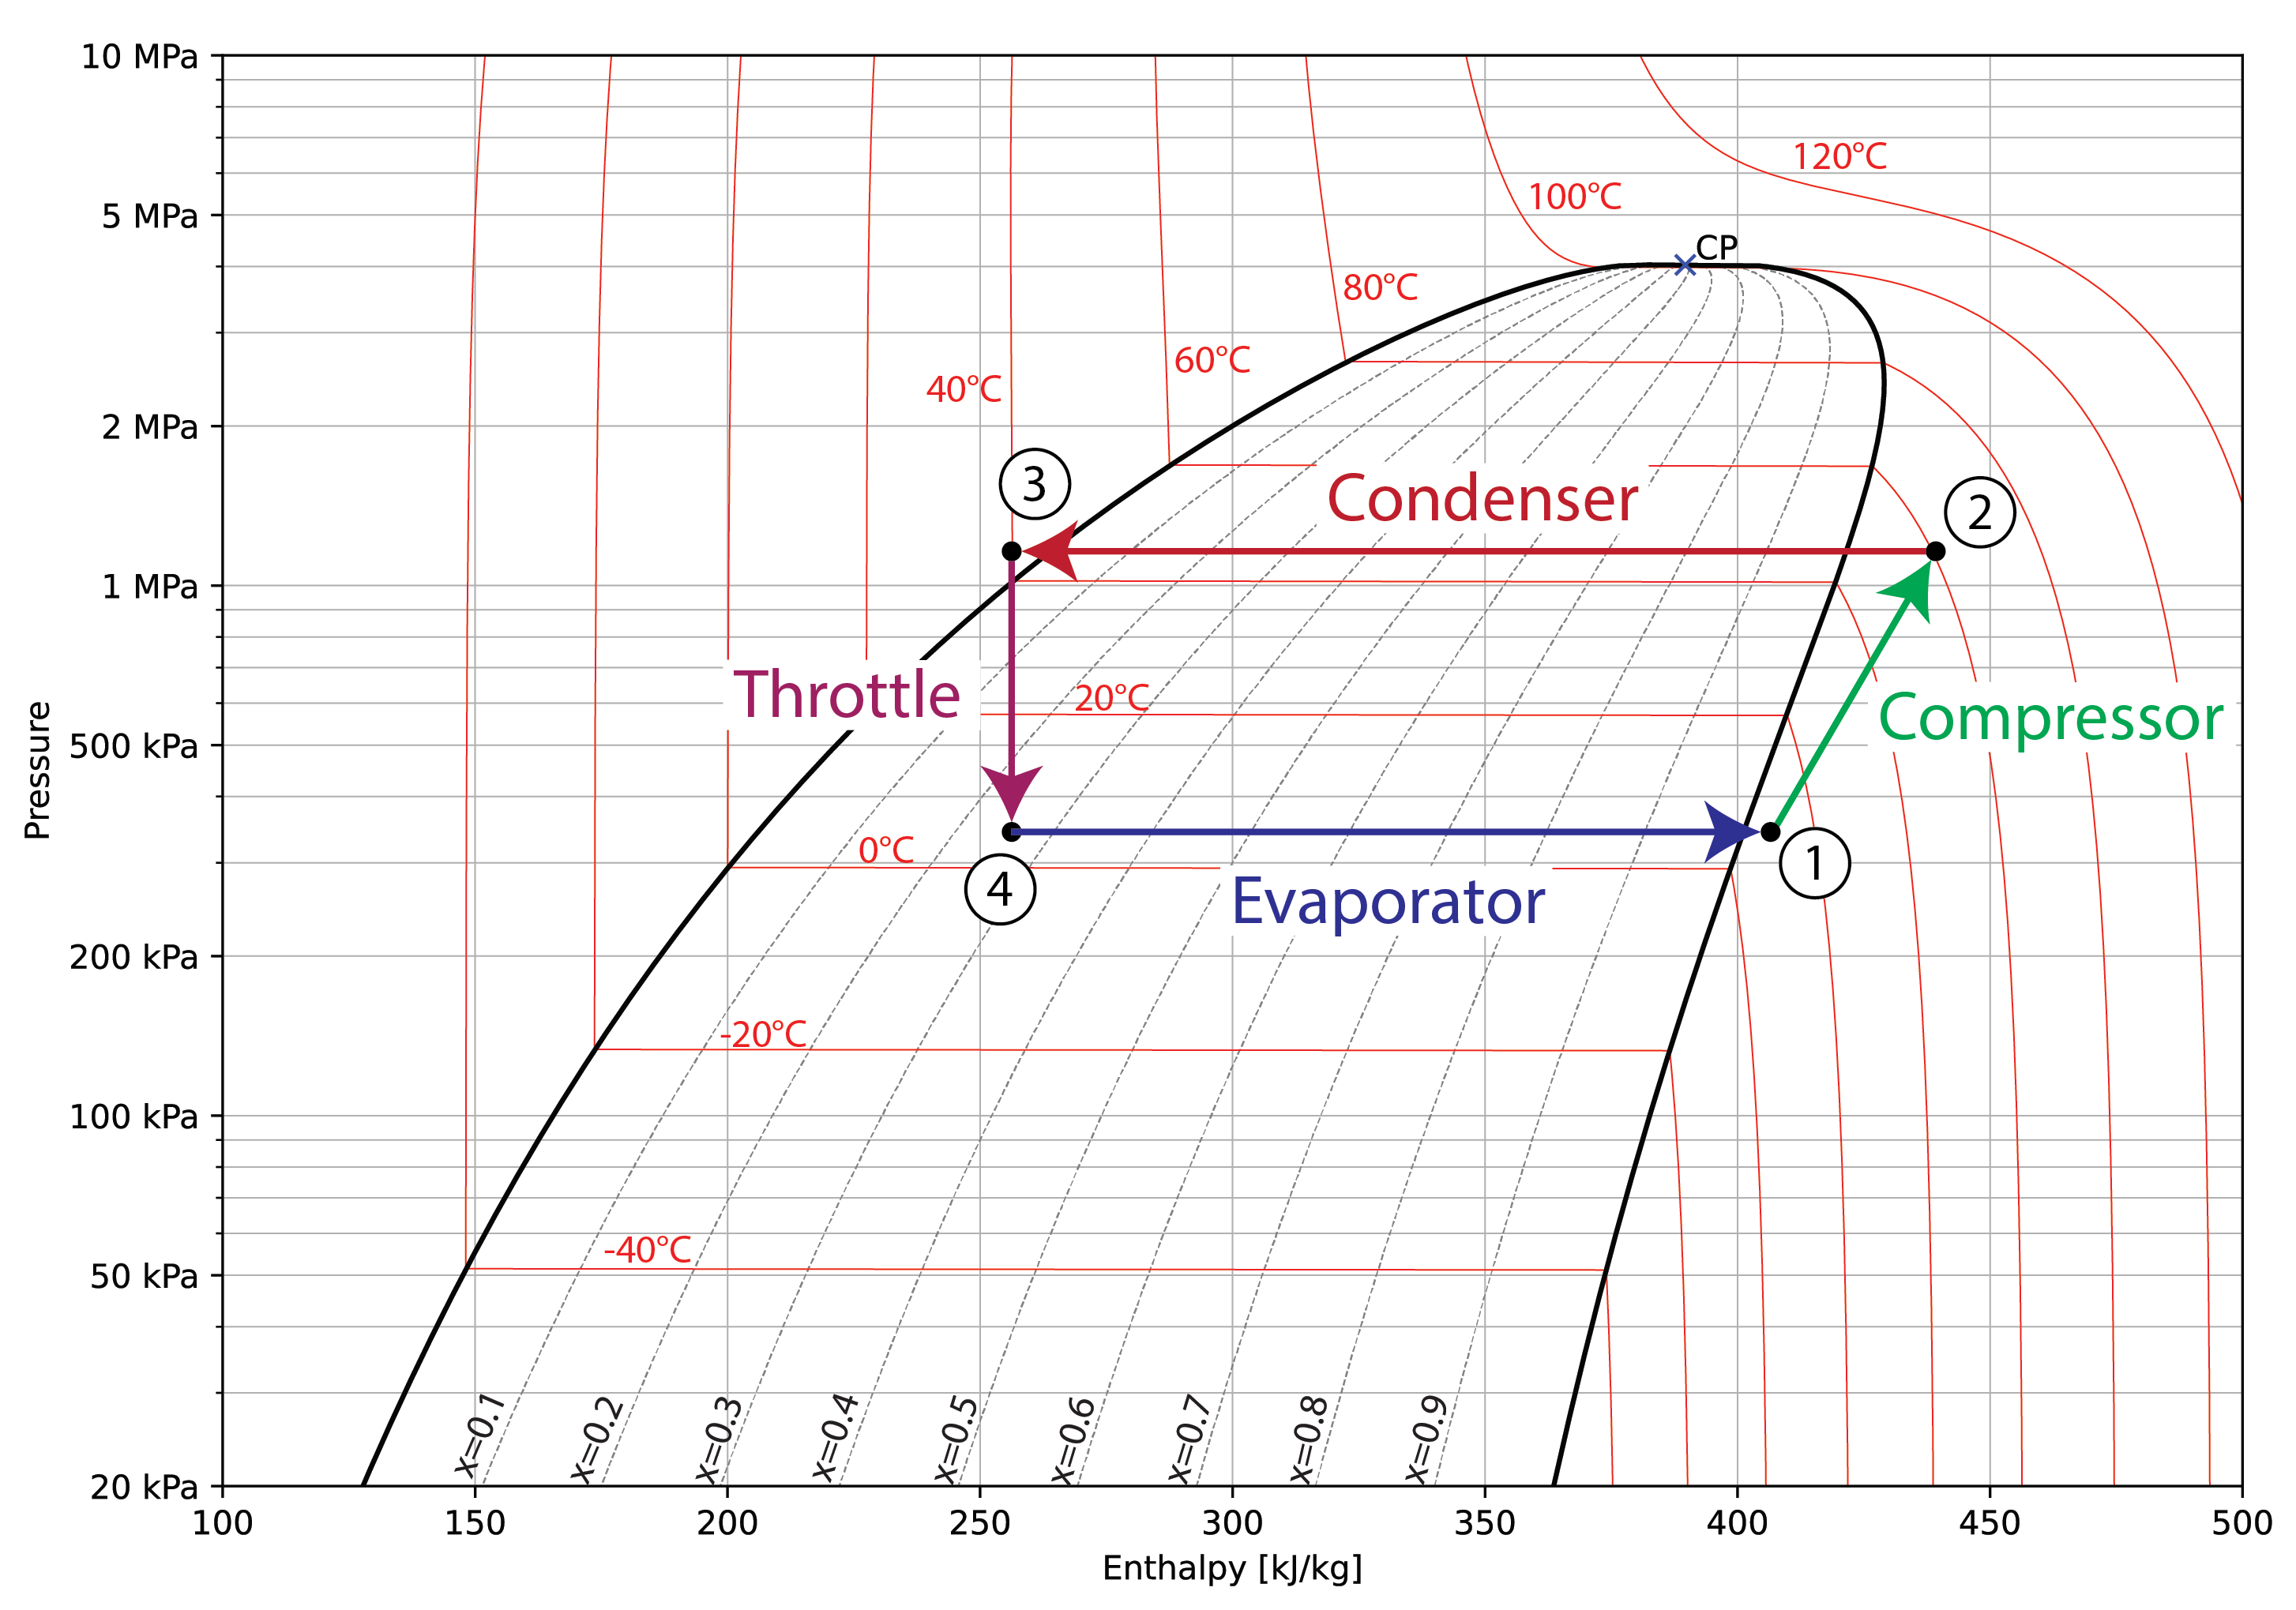
\includegraphics[width=0.9\textwidth]{RefrigerationExampleph}
    %\caption{The states and processes of the refrigeration cycle shown on a $p$-$h$ diagram.}
    %\label{fig:ch4_Refrigerationph}
  \end{figure}

  \subsubsection*{Property Table}

  We now know the pressure and temperature of each state, but this is actually not enough to define the enthalpy of State 4, as it is in the saturated region.  Fortunately, because Process 3-4 is a throttle (which are isenthalpic), the enthalpy of State 4 will be equivalent to that of State 3.  As before, CoolProp is used for all enthalpies, properties in black are taken from the problem statement, and quantities in red are calculated.

  \begin{table}[H]
    \centering
    \def\arraystretch{1.5}
    %\caption{Tabular Representation of Energy Equation for Stirling Cycle}
    %\label{tab:ch3_stirling}
    \begin{tabular}{r|cccc}
      & State 1 & State 2 & State 3 & State 4 \\ \hline
      Pressure    & {\color{Red} 350 kPa}  & 1.2 MPa  &  1.2 MPa &  {\color{Red} 350 kPa}       \\
      Temperature & 10°C   & 60°C &  40°C   & 5°C  \\
      Enthalpy    & $\color{Red} 406.1\ \frac{\rm kJ}{\rm kg}$ & $\color{Red} 437.8\ \frac{\rm kJ}{\rm kg}$ & $\color{Red} 256.4\ \frac{\rm kJ}{\rm kg}$ & $\color{Red} 256.4\ \frac{\rm kJ}{\rm kg}$ \\
      Quality     & -       & -     &   -      &  0.25
    \end{tabular}
    \def\arraystretch{1.0}
  \end{table}

  Once again, each of the values for enthalpy matches well with the locations of the States in the $p$-$h$ diagram.

  \subsubsection*{Compressor Work, Evaporator/Condenser Heat Transfer}

  Because the compressor is assumed to be adiabatic, and there are no moving parts in the evaporator or condenser, the specific work and heat transfer can be found directly through the difference in enthalpies.

  The compressor sits between States 1 and 2:
  \begin{equation*}
    w_{comp} = h_2 - h_1 = 437.8\ \frac{\rm kJ}{\rm kg} - 406.1\ \frac{\rm kJ}{\rm kg} = \redbox{31.7\ \frac{\rm kJ}{\rm kg}}
  \end{equation*}

  The condenser is between States 2 and 3, and the evaporator is between States 4 and 1:
  \begin{align*}
    q_{cond} &= h_2 - h_3 = 437.8\ \frac{\rm kJ}{\rm kg} - 256.4\ \frac{\rm kJ}{\rm kg}= \redbox{181.4\ \frac{\rm kJ}{\rm kg}} \\
    q_{evap} &= h_1 - h_4 = 406.1\ \frac{\rm kJ}{\rm kg} - 256.4\ \frac{\rm kJ}{\rm kg}= \redbox{149.7\ \frac{\rm kJ}{\rm kg}}
  \end{align*}

  There is no work or heat transfer associated with the throttle.

  \subsubsection*{Coefficients of Performance}
  This system is designed for refrigeration of a living space, so we are primarily interested in the heat absorbed by the evaporator, $q_{evap}$.  This means that the coefficient of performance can be calculated as follows:
  \begin{equation*}
    COP_R = \frac{q_{evap}}{w_{comp}} = \frac{149.7\ \frac{\rm kJ}{\rm kg}}{31.7\ \frac{\rm kJ}{\rm kg}} = 4.72
  \end{equation*}

  This is significantly higher than typical coefficients of performance for residential AC, which usually run between 2 and 4.  Likely, this means that our compressor is too efficient, and a real compressor for this system would require more energy in order to create the same increase in pressure.

  If the goal of this refrigeration unit was instead heating up the inside of the home, and the evaporator and condenser temperatures were exactly the same (reasonable for a chilly day, with an indoor temperature around 20°C), we would instead use the condenser heat transfer to calculate the coefficient of performance:
  \begin{equation*}
    COP_{HP} = \frac{q_{evap}}{w_{comp}} = \frac{181.4\ \frac{\rm kJ}{\rm kg}}{31.7\ \frac{\rm kJ}{\rm kg}} = 5.72
  \end{equation*}

  This value is exactly 1 higher than $COP_R$, which matches our analysis of the Stirling Cooling cycle back in Section \ref{sec:ch3_StirlingCooling}.
  
\end{example}

\section{Summary}
In this chapter, we analyzed several variations of the Rankine Cycle, including both reheat and regeneration.  The Rankine Cycle is commonly used in steam power plants.  Additionally, we looked at the vapor-compression refrigeration cycle, which is commonly used in air conditioning units and refrigerators.

Each of these cycles used the First Law of Thermodynamics, modified for open systems:
\begin{equation*}
  \Delta h = q-w
\end{equation*}

Because we used steam or refrigerant R134a for our examples, we were typically given enough information to find the enthalpies of each state, with only constant pressure processes being used to jump between states.  Tables are provided to calculate these properties through linear interpolation, or CoolProp can be used to find properties directly.

Finally, we considered the efficiency of systems, which is defined as the thermal efficiency, $\eta_{th}$, for power plants, and as the coefficient of performance, $COP_R$ or $COP_{HP}$ for refrigerators or heat pumps:
\begin{align*}
  \eta_{th} &= \frac{w_{net}}{q_{in}} \\
  COP_R &= \frac{q_{evap}}{w_{comp}} \\
  COP_{HP} &= \frac{q_{cond}}{w_{comp}}
\end{align*}

\begin{homework}
  %% Conceptual Questions
  % Section 4.1 (Energy Equation)
  \question Thinking about the energy equation, how do we get the enthalpy term?  What concept gives us the additional term to change $u$ into $h$?
  
  \question What does the dot mean in $\dot{m}$, $\dot{W}$, and $\dot{Q}$?  What units do each of those terms have?
  
  % Section 4.2 (p-h Diagram)
  \question For an adiabatic process, how would we represent work on a $p$-$h$ diagram?
  
  \question Why are the constant temperature lines vertical to the left and right of the $p$-$h$ diagram?  Is enthalpy more dependent on temperature or pressure in those regions?
  
  \question Why is the constant temperature line horizontal in the central point of the diagram?  Assuming constant temperature, what is the primary property that would determine enthalpy in that region?
  
  % Section 4.3 (Components of Thermo Systems)
  \question Which components add or remove energy as work from a system?
  
  \question Which components add or remove energy as heat from a system?
  
  \question Which components move heat within the system?
  
  \question Which components do not add or remove energy as either work or heat?

  \question What limitations are placed on pumps and turbines? (i.e. where in the $p$-$h$ diagram are they allowed to operate?)
  
  % Section 4.4 (Basic Rankine Cycle)
  \question What four components are present in the Rankine cycle?
  
  \question Why do we sometimes neglect the energy to run the pump?
  
  \question How do we define efficiency for a Rankine cycle?  What are we ``getting out'' of the cycle?  What are we ``putting in''?
  
  % Section 4.5 (Rankine with Mods)
  \question What value did the reheat process add?  Thinking about Example \ref{ex:ch4_supercrit}, what would have happened without re-heating?  What would the quality have been at the outlet of the LP turbine?  Is that acceptable for turbines?
  
  \question How did the efficiency equation change when we considered a reheat?
  
  \question What value did regeneration add in Example \ref{ex:ch4FeedwaterHeater}? Without regeneration, what happens to the heat added in the steam generator?  What happens to the total work output? What happens to the efficiency?
  
  % Section 4.6 (Refrigeration)
  \question What has motivated the change in refrigerants over the years?
  
  \question What makes R1234yf preferable to R134a?  What makes it worse?
  
  \question Why do we use a throttle instead of a turbine for a refrigeration cycle?
  
  \question A furnace directly burns fuel to heat homes.  How does this differ from a heat pump?  What about electric space heaters?  For each, what are we paying for to get the end product of heat inside our house?
  
  \question Do refrigerators move heat from cold to hot? If so, how?
  \newpage
  %---------------------------------------------------------------------------
  %% Work-out Questions
  \question A small community of about 500 households have discovered an underground geothermal brine source that can be used to boil water at 100°C and would like to use this to generate power. The following diagram shows the initial design of a low pressure geothermal plant in which the water is boiled by the geothermal source to 100°C and subsequently superheated to 200°C by a wood-fired superheater. Notice that the high pressure of the system is at 100kPa allowing a convenient de-aerator to be placed at the pump outlet.
  \begin{center}
    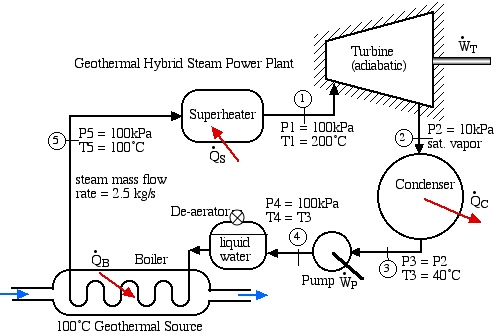
\includegraphics[width=0.75\textwidth]{ch4_HW_geo}
  \end{center}
  \begin{questionparts}
  \item Neatly sketch the complete cycle on the pressure-enthalpy $p$-$h$ diagram for water, indicating clearly all 5 stations on the diagram.
  \item Assuming that the turbine is adiabatic, determine the power output of the turbine \answer{[729kW]}.
  \item Assuming that the feedwater pump is adiabatic, and that the compressed liquid experiences no change in temperature while passing through the pump, determine the power required to drive the pump \answer{ [0.23kW]}.
  \item Using steam tables, determine the heat transferred to the boiler \answer{ [6271kW]} as well as the heat transferred to the superheater \answer{ [500kW]}.
  \item Determine the overall thermal efficiency $\eta_{th}$ of this power plant \answer{ [11\%]}. (Thermal efficiency is defined as the net work done by the system (turbine and feedwater pump) divided by the total heat supplied externally).  Is this the best measure of efficiency for this power plant?
  \item Discuss the proposed system with respect to its environmental impact and feasibility. Is this a well designed system? What do you consider to be the major advantages and disadvantages of this system? Your discussion should include a comparison of the external fuel used and the turbine power.
  \end{questionparts}
\newpage
  \question We wish to evaluate the proposed Solar-Pond Steam Power Plant shown in the following diagram. A solar pond is a large body of water having a varying salinity gradient (halocline) which traps the sun's energy such that the storage layer at the bottom of the pond can reach temperatures of greater than 100°C. The diagram following shows the initial design of a low pressure solar-pond steam power plant, using the storage layer as the boiler heat source, and the upper layer as the heat sink. Notice the wood-fired superheater in which the steam at the outlet of the boiler is heated from 100°C to 250°C.
  \begin{center}
     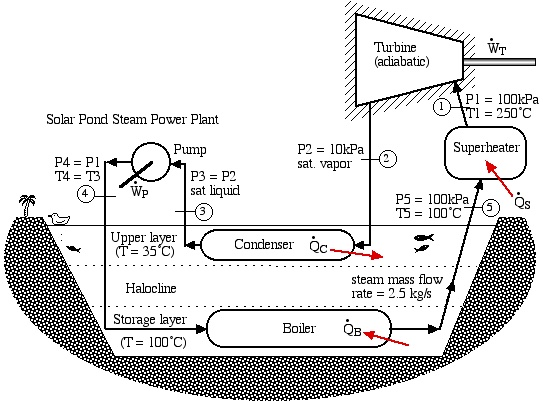
\includegraphics[width=0.75\textwidth]{ch4_HW_solar}
  \end{center}
  \begin{questionparts}
  \item Neatly sketch the complete cycle on the pressure-enthalpy $p$-$h$ diagram for water, indicating clearly all 5 stations on the diagram.
  \item Assuming that the turbine is adiabatic, determine the power output of the turbine \answer{ [976kW]}.
  \item Assuming that the feedwater pump is adiabatic, and that the compressed liquid experiences no change in temperature while passing through the pump, determine the power required to drive the pump \answer{ [0.23kW]}.
  \item Using steam tables, determine the heat transferred to the boiler \answer{ [6210kW]} as well as the heat transferred to the superheater \answer{ [747kW]}.
  \item Determine the overall thermal efficiency $\eta_{th}$ of this power plant \answer{ [14\%]}. (Thermal efficiency is defined as the net work done by the system (turbine and feedwater pump) divided by the total heat supplied externally).  Is this the best measure of efficiency for this power plant?
  \item Discuss the proposed system with respect to its environmental impact and feasibility. Is this a well designed system? What do you consider to be the major advantages and disadvantages of this system? Your discussion should include a comparison of the external fuel used and the turbine power.
  \end{questionparts}
  \question In an effort to decentralize the power grid and utilize the waste heat which accompanies power generation, the Athenai Power Consulting Corp. has proposed a Cogeneration system for O'Bleness Hospital to provide both 500 kW electric power and hot water at 60°C. The basic approach to this unique design is shown in the following schematic diagram:
  \begin{center}
    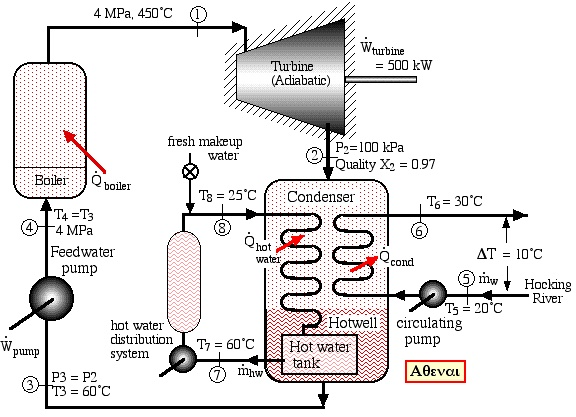
\includegraphics[width=0.75\textwidth]{ch4_HW_cogen}
  \end{center}
  \begin{questionparts}
  \item Neatly sketch the complete cycle on the pressure-enthalpy $p$-$h$ diagram for water, indicating clearly all 8 stations on the diagram.
  \item Determine the mass flow rate of the steam through the cycle required in order to provide the turbine output power of 500kW \answer{[0.691 kg/s]}.
  \item Determine the power required to drive the feedwater pump \answer{ [2.69 kW]}.
  \item Determine the overall thermal efficiency $\eta_{th}$ of this power plant. (Recall that thermal efficiency is defined as the net work done divided by the total heat supplied externally to the boiler \answer{[23\%]}.
  \item Determine the cooling power in the condenser required to condense the steam exiting the turbine at station (2) and subcool the condensed steam to 60°C at station (3) \answer{[1628 kW]}.
  \item Assuming that the water in the hot water distribution system is heated from 25°C to 60°C, and that no river cooling is provided, determine the mass flow rate of the hot water required to subcool the condenser water to 60°C \answer{ [11.1 kg/s]}
  \item In the lull period when no hot water is required, determine the mass flow rate of water from the Hocking River required to subcool the condenser water to 60°C. Note that the river water temperature rise must not exceed 10°C \answer{ [39 kg/s]}.
  \item Discuss the proposed system with respect to its environmental impact and feasibility.
  \end{questionparts}
  \question We wish to do a preliminary thermodynamic evaluation of a refrigeration system designed for home usage which will use refrigerant R134a. Consider the following system flow diagram:
  \begin{center}
    \includegraphics[width=0.75\textwidth]{ch4_HW_refrig}
  \end{center}
  \begin{questionparts}
  \item Neatly sketch the complete cycle on the pressure-enthalpy $p$-$h$ diagram for R134a, indicating clearly all 4 stations on the diagram.
  \item Determine the work done by the compressor \answer{ [54 kJ/kg]}.
  \item Determine the heat absorbed by the evaporator \answer{ [137 kJ/kg]}, and that rejected by the condenser \answer{ [191 kJ/kg]}.
  \item Determine the Coefficient of Performance of the refrigerator ($COP_R$) (defined as the heat absorbed in the evaporator divided by the work done on the compressor - always presented as a positive value even though the work done $w_c$ is negative) \answer{[$COP_R$ = 2.53]}.
  \end{questionparts}
  \newpage
  \question It is common practice in the refrigeration industry to use an internal heat exchanger to subcool the refrigerant at the outlet of the condenser by means of the refrigerant exiting the evaporator. This practice obtains a much larger refrigeration capacity using the same components.

  Continuing the previous problem, we will add a heat exchanger as indicated.
  \begin{center}
    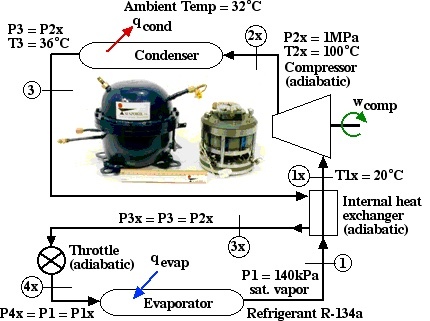
\includegraphics[width=0.75\textwidth]{ch4_HW_refrigHX}
  \end{center}

  Notice that we have included an internal heat exchanger that heats the refrigerant exiting the evaporator (as a saturated vapor at 140kPa) to 20°C. We have chosen a state numbering system (1x, 2x, and so on) so as to allow the new system to be plotted on the same $p$-$h$ diagram as above, and thus to be able to qualitatively compare the increase and improvement of performance provided by adding the internal heat exchanger.
  \begin{questionparts}
  \item Add the 4 states (1x, 2x, 3x, 4x) to the pressure-enthalpy $p$-$h$ diagram from the previous problem and sketch the new cycle.
  \item Determine the heat transferred in the internal heat exchanger, assuming it to be externally adiabatic \answer{ [32.2 kJ/kg]}, and the temperature of the subcooled liquid entering the throttle (3x) \answer{[13.4°C]}.  The heat transferred can be calculated through the equation:
    \begin{equation*}
      q = h_{1x} - h_1 = h_3 - h_{3x}
    \end{equation*}
  \item Determine the heat absorbed by the evaporator \answer{[169 kJ/kg]}.
  \item Determine the heat rejected by the condenser \answer{[235 kJ/kg]}.
  \item Determine the Coefficient of Performance of the refrigerator ($COP_R$) (defined as the heat absorbed in the evaporator divided by the work done on the compressor) \answer{[$COP_R$ = 2.65].}
  \end{questionparts}

  \newpage
  \question We wish to do a preliminary thermodynamic evaluation of a 1kW input power home heat pump system for space heating using refrigerant R134a. Consider the following system flow diagram:
  \begin{center}
    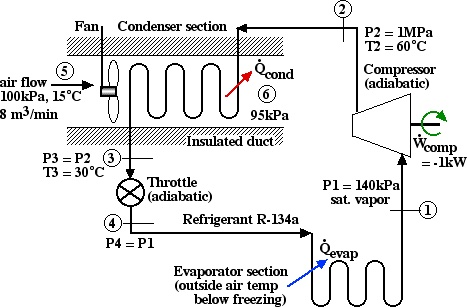
\includegraphics[width=0.75\textwidth]{ch4_HW_heatpump}
  \end{center}

  Thus the heat pump system absorbs heat from the evaporator placed outside in order to pump heat into the air flowing through the insulated duct over the condenser section. The fan provides an air flow of 8 ${\rm m^3/min}$, which is enough to cool the refrigerant in the condenser to 30°C, In this analysis we will neglect the power provided to the fan. We also assume that the duct is adiabatic, and that all the heat rejected by the condenser is absorbed by the air flowing in the duct.

  \begin{questionparts}
  \item Neatly sketch the complete cycle on the pressure-enthalpy $p$-$h$ diagram for R134a, indicating clearly all 4 stations on the diagram (stations 5 and 6 are air, and are therefore not on the same $p$-$h$ diagram).
  \item Determine the mass flow rate of the refrigerant R134a \answer{[0.0185kg/s]}.
  \item Determine the mass flow rate of the air flowing in the insulated duct \answer{[0.161kg/s]}.
  \item Determine the heat rejected by the condenser \answer{[3.7kW]}. Assuming that all this heat is absorbed by the air, determine the exit temperature of the air at station (6) \answer{[37.9°C]}. Is this value reasonable? Why?
  \item Determine the heat absorbed by the evaporator \answer{[2.7kW]}.
  \item Determine the Coefficient of Performance of the heat pump ($COP_{HP}$) (defined as the heat rejected by the condenser divided by the work done on the compressor) \answer{[3.7]}.
  \end{questionparts}

  \newpage
  \question We wish to do a preliminary thermodynamic evaluation of a 500W input power home heat pump system as applied to summertime use for both hot water heating to 50°C, and space cooling (air conditioning), and thus maintain the inside home temperature at a comfortable 20°C.

  \begin{center}
    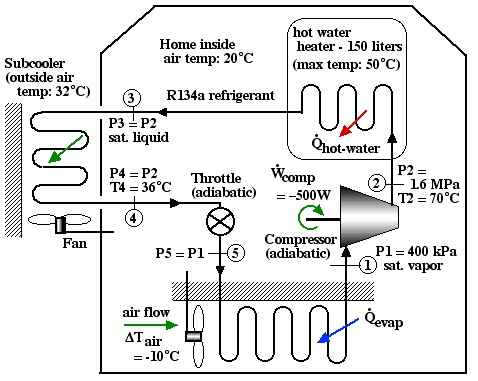
\includegraphics[width=0.75\textwidth]{ch4_HW_AC}
  \end{center}

  This unique combined air conditioning / hot water heating system is designed to absorb heat from the air flowing through the insulated duct in order to pump heat into the hot water heating tank. The fan provides enough air flow over the evaporator to cool the air by 10°C as it passes through the duct, and the hot water is heated to a maximum of 50°C. In this analysis we neglect the power provided to the fan. We also assume that both the duct and the hot water tank are externally adiabatic.
  
  \begin{questionparts}
  \item Neatly sketch the complete cycle on the pressure-enthalpy $p$-$h$ diagram for R134a, indicating clearly all 5 stations on the diagram.
  \item Determine the enthalpy values at all five stations [kJ/kg], and indicate these values on the $p$-$h$ diagram.
  \item Determine the mass flow rate of the refrigerant R134a \answer{[0.0133 kg/s]}.
  \item Determine the heat rejected by the condenser \answer{[2.09 kW]}. Assuming that all this heat is absorbed by the water in the hot water tank, determine the time taken for 150 liters of water at 30°C to reach the required temperature of 50°C \answer{[1 hr 40 min]}.
  \item Determine the heat power absorbed by the refrigerant in the evaporator \answer{[2.04 kW]}. Assuming that all this heat is absorbed from the air in the duct and neglecting the fan power, determine the required mass flow rate of the in order reduce the air temperature by 10°C while passing through the duct \answer{[0.204 kg/s]}.
  \item Determine the Coefficient of Performance of the hot water heater ($COP_{HW}$) (defined as the heat rejected by the condenser divided by the work done on the compressor) \answer{[$COP_{HW}$ = 4.17]}.
  \item Determine the Coefficient of Performance of the air conditioner ($COP_{AC}$) (defined as the heat absorbed by the evaporator divided by the work done on the compressor) \answer{[$COP_{AC}$ = 4.07]}.
  \item If we bypass the outside subcooler (State (4) becomes saturated liquid as in State (3)) determine the change in Coefficient of Performance of the air conditioner evaluated above. Indicate this change on the $p$-$h$ diagram and discuss the relevance of the outside subcooling section in this system. \answer{[$COP_{AC}$ reduced to 3.17]}.
  \end{questionparts}
\end{homework}

